
\documentclass{class}

\usepackage{bbm}

\usetikzlibrary{positioning}

\begin{document}

\renewcommand{\baselinestretch}{1.5} 


\begin{titlepage}
\title{Peak Load Pricing Theory with Incomplete Information}

\author{Leopold Monjoie}

\institute{Aalto University\\ \and
 \email{leopold.monjoie@aalto.fi}}
\date{\today}
\maketitle
\begin{abstract}
\noindent This paper examines the challenges of allocating a good subject to capacity constraints such as electricity when considering consumer preferences and investment decisions. A theoretical framework is developed where a market designer sequentially chooses a level of investment and proposes an allocation mechanism to consumers followed by a consumption stage. The market designer uses the allocation to maximize consumer surplus and finance the investment cost. He faces heterogeneous consumers who have private information about their demand level and belong to a publicly observed category, allowing the market designer to distinguish groups of consumers such as households or industries. We show that the optimal allocation implies discriminating against consumers based on their types and categories and that the relative discrimination depends on the level of investment considered. It has significant welfare and distributive implications: an optimal pricing mechanism can minimize the investment cost and lead to a higher aggregate consumer surplus. However, it is not always a Pareto improvement for every consumer, especially for smaller ones. We describe two main environments: the current second-best situation, in which the market designer cannot obtain information about consumers and must choose fixed prices ex-ante, and the optimal theoretical second-best allocation mechanism that considers the incentive and individual rationality constraints and the investment decisions.

\bigskip
\end{abstract}
\setcounter{page}{0}
\thispagestyle{empty}
\end{titlepage}
\pagebreak \newpage


\section{Introduction}\label{chap3sec:sec1}

% Since # has an increasing marginal welfare cost and a decreasing marginal welfare benefit,W(#) is quasi-concave.

Economists have long advocated that pricing mechanisms should be carefully designed to allow the coverage of investment costs and promote efficient resource use. This is particularly true when providing \textit{essential goods} characterized by the public-good nature of investment availability when supply is scarce, such as electricity, public transport, or medical goods. In those sectors, demand and supply fluctuate unpredictably, and if any demand exceeds the available capacity and cannot be efficiently rationed, it generates significant welfare losses.
% \footnote{This inefficient rationing usually stems from market designers using price regulations, for instance, price caps, or because they are reluctant to implement complex pricing mechanisms due to technical, political, or equity reasons.} 
For instance, without sufficient investment, the reliability of the electricity supply can be compromised, leading to frequent outages and power interruptions \citep{IEA2020}. It is particularly important in the energy transition context. Indeed, it is crucial to lower the production from fossil fuels but reliable technology and invest massively in carbon-free but intermittent renewables. Moreover, the electrification of end-use consumption also implies that periods of scarcity may occur more often. Therefore, we must carefully design electricity markets by choosing the most efficient pricing mechanisms, allowing for sufficient investment and ensuring demand reacts to scarcity \citep{IEA2021}.
% \footnote{Transportation and distribution infrastructure are also central in current policymakers' debates. Network tariffs are usually designed to cover transmission lines' investment and operation costs. Still, the growing share of decentralized production and the intermittent nature of renewable production create new challenges\citep{Eurelectric2021}. The increase of volatility from both the supply and demand-side implies that the sizing of networks must be rethought. Adding a new line to satisfy a high-magnitude but rare event is not necessarily optimal. In this case, the incentive to better size the network can also come through incentives through tariffs.} 
The COVID crisis has also shown that the lack of production capacity for medical goods, especially vaccines, has severe consequences. The absence of sufficient capacity to produce vaccines led to a worldwide lockdown and border closures, increasing contagions and hospital congestion.
% \footnote{For instance, \cite{Kominers2022} and \cite{Athey2022} showed that the price incentives for providing new vaccines and expanding production capacities were largely sub-efficient compared to their social value. On the other hand, the crisis also highlights the issue of who should be allocated the vaccines, given the scarcity of available production capacity. In this context, \cite{akbarpour2023economic} underlined that the classic opposition between prices and free, but random, allocation is not straightforward.} 
Finally, congestion in transportation systems continues to generate substantial costs \citep{schrank2021} and poses challenges for the much-needed modal shift to low-carbon means \citep{ITDP2021}.
% \footnote{Increasing prices for fossil fuel vehicles would reduce pollution and generate revenue to invest in decarbonized means. On the other hand, if we want to encourage consumers to use carbon-free transport solutions, their pricing should also be carefully designed, especially to avoid congestion costs.}

In this paper, we provide a framework highlighting the inherent tensions that arise when implementing an allocation mechanism that dictates how agents consume the goods, and generates revenue to finance new investments in an incomplete information framework with heterogeneous consumers.  Numerous theoretical contributions have been made to understand the importance of having sufficient investment.\footnote{Namely, how to implement mechanisms to procure sufficient investment at the least cost and consider the private incentives producers face, which may differ from the optimum. Those mechanisms can range from direct subsidies to the design of more complex competitive markets. An important stream of literature in electricity markets is focused on studying long-term markets in which producers offer either future production via long-term contracts \citep{ausubel2010using} or their future availability through, for instance, capacity remuneration mechanisms \citep{leautier2016visible,holmberg2020optimal}.} Nonetheless, they are mainly centered around the supply-side of the problem and consider the demand as given. Therefore, the first contribution of this paper is to discuss the implications of considering the demand-side when it comes to ensuring an efficient level of investment. We provide a model to analyze the interaction between a set of heterogeneous consumers, the choice of the pricing mechanism, and the use of the revenue generated through this mechanism to increase available capacity. The use of consumer heterogeneity allows us to raise the issues of the redistribution generated by an allocation mechanism that is considered more efficient. We find that reaching a certain level of investment that maximizes aggregate consumer surplus and implementing the corresponding allocation mechanism to finance the investment can lead to different welfare levels depending on the consumer types. This means the most efficient mechanism is not always Pareto-improving for every consumer, even considering an increase in available capacity.\footnote{For clarity, we do not discuss in this current paper version the optimal level of investment. While this provides both technical and policy results, it mainly boils down to comparing the different, and sometimes opposite, effects that are described in this paper.}

The second contribution lies in the assumption that the utility buyers derive from consuming the goods is private information. The consumers are characterized by a linear marginal utility function, which is uncertain when the market designer makes investment decisions and proposes an allocation mechanism. This uncertainty has two additive components: (i) a common shock that is identical across all consumers, and (ii) a private shock only observed by consumers before the consumption stage and the realization of the common shock. We also embedded each consumer with a category for which the market designer is publicly informed.\footnote{The support of the distribution of a consumer type depends on the category to which he belongs.} The existence of private information with respect to their consumption implies that consumers' private incentives might also differ from the market designer's objective. Therefore, the allocation mechanism in the framework can be used simultaneously to generate revenue to cover investment costs and screen for unobservable characteristics to ensure efficient consumption. 

The supply side is represented by a market designer, which can be interpreted as a public authority or a regulated monopoly, that (i) determines the allocation in prices and quantities of a homogeneous good and (ii) chooses the level of investment that maximizes consumer surplus. The allocation mechanism defines the monetary transfer and the quantity for a set of consumers during the consumption stage subject to capacity constraint. Therefore, when the market designer chooses the mechanism, he must consider that demand may exceed the level of available capacity and that specific actions need to be taken to reduce aggregate consumption. This creates an asymmetric effect of the optimal allocation when the capacity is binding or not. Hence, the consideration of the capacity constraint significantly impacts the design of the efficient mechanism and the revenue generated by the mechanism.\footnote{In this paper, the capacity constraint is hard in the sense that we do not represent the costs associated with demand exceeding available supply. Therefore, the market designer can always reduce demand but at the cost of misallocation due to imperfect information. Several papers have described those costs in more detail, such as rolling blackouts in electricity \citep{fabra2018primer,llobet2018conventional} or congestion costs in transports \citep{YOSHIDA2008228,DEPALMA2017106}.}  We also describe the (potential) incompleteness of the mechanism proposed by the market designer due to implementation constraints.\footnote{We mean by implementation constraints an environment in which the market designer cannot set the optimal allocation for every demand realization.} Finally, note that as the market designer uses the allocation to maximize consumer surplus and finance the investment cost, he is also under a revenue constraint. 

We analyze several market design environments to highlight the range of mechanisms at play in this framework. In section \ref{chap3sec:sec3}, we start with the first-best, in which the market designer perfectly observes the consumer type when choosing the investment level and the allocation. Including heterogeneity in the canonical model does not alter the fundamentals of the pricing decision: the optimal mechanism can be directly implemented by a spot market, with a unique (unitary) monetary transfer from each consumer. Section \ref{chap3sec:sec4} analyzes the \textit{current} second-best implemented across many markets. The market designer faces private information about the level of consumption and is constrained in the monetary transfer he can implement. Namely, the price is unique for every state of the world, and it can vary based on the category of consumers. One of the main results is the non-monotonous relation between the price of the smaller consumers' category and the level of investment. For small levels of investment, the price decreases in the level of investment, and then beyond a specific value, it increases similarly to the price of the biggers' category. The cause lies in the relation between the market designer's objective and the constraints he faces. Increasing the level of investment changes the capacity constraint. In turn, it modifies the utility marginal rates of substitution between the different categories of consumers in favor of the category of smaller consumers. This effect fades away for high levels of investment as the gain from a marginal increase in the level of investment is lower. On the other hand, the financing cost is convex in the investment level; that is, the budget constraint is increasingly tightening. It explains why, for small levels of investment, the consumer surplus effect dominates, while the revenue effect dominates for high levels. Finally, in section \ref{chap3sec:sec5}, we look at the theoretical second-best case under incomplete information and we implement a mechanism design approach. In that environment, the market designer proposes an individual contract that needs to satisfy the incentive compatibility constraint in addition to the previous ones. The main results are that the market designer discriminates against consumers based on their type and it can be observed both in terms of quantity and individual welfare. For consumers with smaller consumption, an increase in the level of investment can lead to a decrease in the allocated quantity. On the other hand, only sufficiently big consumers have both an increase in quantity and in their welfare when the level of investment increases. The relation between the quantity allocated and the level of investment is based on the interaction between the revenue and consumer surplus effect described in Section \ref{chap3sec:sec5} and the consumers' virtual marginal utility, which takes into account the cost associated with truthful behavior. For a given consumer type, the individual welfare effect is based on the information rent, which itself relies on the quantity allocated to smaller consumers. The remainder of this section discusses the related literature. Section \ref{chap3sec:sec2} presents the environment.

\textbf{Related Literature}

We build the framework on several strands of literature. The dynamic interaction between investment decisions and the consumption stages stems from the \textit{peak-load pricing theory} that originated from \cite{m1949tarification}. It describes how capacity constraints interact with the provisions of a homogeneous good with time-varying uncertain stochastic demand.  It has mainly been used in recent work to study the role of market power, as in \cite{leautier2016visible}, where producers can increase the price on the spot market beyond marginal cost even though they are not capacity-constrained. The effect of price regulation is also analyzed in \cite{leautier2018long}, where the author demonstrates that short-term inefficiencies can sometimes have long-term and counterintuitive effects. In this paper, the price cap changes the private incentives producers face, hence the final investment decisions. \cite{holmberg2020optimal} study the effect of having inefficient rationing. Consequently, electricity prices do not internalize this additional cost, and the market designer needs to implement an additional stream of revenue for the producers. This work introduces two features in the model: (i) heterogeneous consumers with private information and (ii) inefficiencies due to the schedule commitment by the market designer before the uncertainty is resolved.\footnote{This work mirrors the literature from congestion pricing theory from \cite{vickrey1963pricing,vickrey1969congestion}. For a recent theoretical paper, see, for instance, \cite{DEPALMA2017106}, which also compares different allocation mechanisms but without considering the demand-side.}

This paper is also based on a second stream of papers that is related to the electricity markets and is based on the seminal paper by \cite{chao1987priority} on priority service. The central idea is to provide a mechanism design solution in the form of a contractual arrangement where consumers choose the allocation during the wholesale market at the same time. It is in the same vein as the allocation schedule of this paper and the probability of being disconnected when demand exceeds the level of capacity. This framework has been refined by a series of papers by the same authors, including the comparison with other market arrangements \citep{chao2022priority} and the role of risk aversion \citep{chao2012competitive}. We also relate to a series of papers focusing on implementing the second-best pricing method for consumers with incomplete information in \cite{spulber1992capacity,spulber1992optimal,spulber1993monopoly}. The work in \cite{spulber1992optimal} focuses on an incomplete information framework without endogenous investment decisions. The optimal allocation schedule is non-linear because consumers' type is private information. Therefore, the market designer faces some challenges when implementing such schedules. In \cite{spulber1992capacity}, a regulated firm is introduced to consider its revenue constraint. However, the focus of this paper remains circumscribed to the design of consumers' second-best tariffs. Finally, \cite{spulber1993monopoly} studies the case of a monopoly designing the rates under incomplete information. We depart from this literature by deepening the private incentives consumers might have by behaving strategically from the truthful reporting and by tightening the link with the investment decisions framework developed in the previous paragraph.

Most of the recent empirical works on redistribution study the short-term effect of pricing issues without considering the long-term interactions with the level of investment. This issue has been recently studied in several empirical papers in the context of essential goods. For instance, in electricity markets, \cite{cahana2022distributional} explore the redistributive effects of switching from a flat electricity price to real-time pricing. Depending on the design, low-income households may lose due to specific consumption patterns in the face of available supply.\footnote{\cite{levinson2022electric} have studied the rates implemented by utilities in the U.S. and how they take into account redistribution preferences in their design. Due to the rapid increase in residential rooftop solar photovoltaic, electricity network tariffs have also been studied, notably in the Californian markets. If the tariffs are mostly based on variable parts, then non-adopters tend to cross-subsidies adopters of such technologies. One central issue is that the latter are mostly high-income households \citep{burger2020quantifying}.} Concerning medical goods, the scarcity of vaccines creates a trade-off between protecting the most vulnerable (e.g., elderly), the likely spreader (e.g., students), or the individual bringing the highest economic benefits (e.g., front-line health workers).
% \footnote{\cite{Sudarmawan2022} shows how countries choose who should receive the vaccine first. \cite{rahmandad2022behavioral} describes the trade-off of allocating the vaccines between the most vulnerable and the high-transmission individuals. Finally, \cite{Persad2020} discusses the ethical consideration of allocating vaccines.} 
Finally, in the case of congestion pricing, \cite{hall2021can} studies the pricing of a lane portion. Using survey and travel time data, the author finds that a fully efficient toll is unnecessary for sufficient welfare and Pareto improvement. 

From a theoretical perspective, the issues related to distributive concerns are borrowed from a growing body of literature using mechanism design.
% \footnote{This paper fits within the new literature on industrial organization using an incomplete information framework. Triple-IO (for Incomplete Information Industrial Organization) papers aim to underline traditional industrial organization issues and how they can be renewed when imperfect information exists. See, for instance, the literature review by \cite{loertscher2021incomplete}. This paper deals with the effect of capacity-constrained systems where (inefficient) rationing must be implemented. It fits with some works by \cite{loertscher2020monopoly,loertscher2021wage} and \cite{gilbert2000equilibrium}, which studies pricing and rationing decisions within imperfect information. We add to the existing literature by providing a similar framework but by including investment decisions and a different type of rationing mechanism.} 
In particular, \cite{akbarpour2023economic} and \cite{akbarpour2023redistributive} provide a framework with consumers' characteristics, such as the private information and the publicly-observed categories, in line with the current paper. They study the trade-off between allocating certain vaccines on a free but random basis or using prices to discriminate and extract information from consumers. The authors assume that the market designer has distributive and exogenous revenue preferences. Therefore, the model exhibits a tension of allocating the good via prices, which generates some revenue, or via a random free allocation that minimizes distributive issues. This paper endogenizes the revenue preference by implementing investment decisions with a revenue constraint. We also provide results when the market designer can imperfectly implement prices. Finally, a recent paper by \cite{crampespricing} studies the implementation of an optimal Pareto income tax schedule \textit{à la Mirrlees} when considering the interaction between consuming energy services (heating, air conditioning, light) and investing in energy efficiency with incomplete information about consumer utility. This paper has a similar spirit, but the link between consumption and production capacity fundamentally differs.


\section{Environment}\label{chap3sec:sec2}

Although the terminology is tailored to electricity, the results can, with some modifications, be applied to other essential goods, as noted in the introduction. 

Our framework consists of five elements: 
(i) the demand side, which may represent households, industrial consumers, or retailers; 
(ii) the allocation mechanism, which specifies how the market designer allocates electricity in terms of both quantity and monetary transfer; 
(iii) the supply side, which captures investment and production decisions;
(iv) the objective function of the market designer; and 
(v) the timing of decisions.

\noindent \textbf{Consumers Preferences} 

\noindent There is a unit mass of consumers for electricity. Each consumer is characterized by a type vector $(i,\theta,s,\lambda)$. We assume that the three dimensions of the vector $(i,\theta,\lambda)$ have a joint distribution among consumers and are known by the market designer. The first characteristic refers to the consumer category, e.g., household or industry. There is a finite set of categories such that $i \in N = \{1,...,n\}$. It is publicly observed, and the size of each category, i.e., the number of agents, is denoted by $\mu_i>0$ for each group. The second characteristic is consumer private preference $\theta$, which, under an incomplete information framework, is assumed to be observed only by the consumer. Conditional on belonging to a category $i$, this value is drawn from a common-knowledge cumulative distribution function $G_i$ whose continuous density is $g_i>0$ has full support on $\Theta_i$ and is strictly positive on $[\ubar{\theta}_i, \overline{\theta}_i]$. With households, $\theta$ represents the revenue shocks, the lowest type of consumer being the poor household, and the highest type of consumer being the more prosperous household. Industrial consumers could also be modeled with this framework, where $\theta$ represents their buyers' orders. The characteristic $s \in S = [\underline{s},\overline{s}]$ represents the state of the world and introduces demand uncertainty. We assume that all consumers are subject to the same shock $s$ and that the market designer's redistributive preferences do not depend on the realization of $s$. It is common knowledge among all agents. Economically, $s$ can capture, for example, a weather condition or a macroeconomic factor. The shock is drawn from a continuous distribution $F$ with density $f>0$, both of which are common knowledge before the shock is realized, and has full support on $S$. Each consumer type is known before the demand shocks are realized. Therefore, this framework encompasses two interpretations of the demand shocks: (i) a static model with a single shock and there is uncertainty concerning its realization, or a (ii) a repetition of multiple shocks over a given period (for example, one year), which are drawn from the distribution $F(.)$ \citep{leautier2016visible}. In the last interpretation, we assume that the consumer type does not change across shocks and is determined before this period. Finally, $\lambda \in \mathbb{R}_+$ are the market designer welfare weights for a given individual. As for the type $\theta$, we assume that this information is private and unobserved by the market designer. All agents in the game are considered to be risk-neutral.

We define a consumer's utility belonging to a category $i$ of a type $\theta_i$. The value for electricity consumption for each consumer is denoted: 

\begin{equation*}
    \theta \theta \; U(q,s) = \theta\int_0^{q} u(\tilde{q},s) d\tilde{q}
\end{equation*}

With $q$ the quantity of electricity allocated to the consumer. If a consumer does not receive electricity, its value is null: $U(0,s) = 0$. $u$ is the marginal willingness to pay for a given quantity of electricity. $u$ specification satisfies the Spence–Mirrlees condition that marginal willingness to pay is strictly increasing in type: higher types prefer larger allocations for any given quantity. All consumers should be allocated at least some quantity $\lim_{q\downarrow0}\theta \; U(q,s)= \infty$, that higher $s$ leads to higher willingness to pay and the marginal utility is decreasing in $q$: $u_{\theta}>0,u_{s}>0,u_{q}<0$.  A consumer receives a quantity $q$ in exchange for a monetary transfer $t$. We assume transfers are separable, and there are no income effects. Each consumer participates in the market if its expected surplus is nonnegative;

\[%%%%%%%%%%%%%%%%%%%
\; \E_{s}\!\big[\,\theta \; U(q_i(\theta,s),s) - t_i(\theta,s)\,\big]
\;\ge\; 0,
\qquad \forall\, \theta\in\Theta_i. \tag{IR}\label{IR-def}
\]%%%%%%%%%%%%%%%%%%%

\noindent \textbf{Allocation Design} 

\noindent We derive different mechanisms to allocate electricity. We distinguish between a \textit{general mechanism} and some \textit{market mechanisms}. In the former, the market designer independently selects the quantity and the monetary transfer, which serves as our benchmark allocation. In the latter, the market designer offers a transfer schedule, and consumers choose their preferred quantity. We now define these formally.

\noindent \textbf{General Mechanism}. Given a total quantity $Q(s)$ of electricity in state $s$, a general allocation mechanism $\mathcal{M}$  consists of collection of functions $q_i: [\ubar{\theta}_i, \overline{\theta}_i]\times S \rightarrow [0,Q(s)] $ where $q_i(\theta,s)$ is the quantity of electricity allocated to a consumer of type $\theta$ in category $i$ at state $s$. The aggregate quantity allocated to a group  $i$ is

\begin{equation*}
    Q_i(s) = \mu_i \E_{\theta_i} [q_i(\theta,s)].
\end{equation*}

Feasibility requires that $Q(s) = \sum_{i} Q_i(s)$. Transfers are described by the functions $t_i(\theta,s)$ assigning a monetary payment to each consumer of type $\theta$ in category $i$ at state $s$. To study the optimal second-best mechanism with incomplete information in section \ref{chap3sec:sec5}, we rely on the Revelation Principle. In a direct mechanism $(q_i,t_i)_{i = \{1,2\}}$, consumers report their type $\theta$, receive an allocation $q_i(\theta,s)$, and pays $t_i(\theta,s)$ to the market designer. 

\noindent \textbf{Market mechanism}. In addition to the general mechanism, we define a \textit{market allocation}, which corresponds to an indirect mechanism. Given a transfer schedule $t(q,\theta,s)$, a consumer chooses a quantity schedule $d(\theta,s)$ as the solution to

\[
d(\theta,s) := \arg\max_q \{ \theta \; U(q,s) - t(q,\theta,s) \}.
\]

Hence, a market allocation is one in which consumers optimally select their allocation given the schedule offered by the designer. We use the notation $d(\theta,s)$ to distinguish this individual demand function from the direct allocation rule $q(\theta,s)$. The comparison between the mechanism design and the market allocation will become handy for different reasons. First, market allocations are the primary mechanism used to allocate electricity in practice. 
They encompass different pricing schemes, such as spot pricing (where $t(q,\theta,s)$ is a unit price resulting from a market-clearing condition) and two-part tariffs (where $t(q,\theta,s)$ consists of a unit price and a lump-sum transfer). Second, having the general mechanism as a benchmark allows for comparing various forms of market allocations, particularly in terms of their implications for consumer surplus. 

\noindent \textbf{Supply side} 

\noindent We assume the most straightforward formulation for the supply-side represented by a single agent, the market designer. It can be interpreted in several ways: as a public firm, as a regulator directly controlling a private monopoly, or as an intermediary between consumers and producers. In the latter case, the mechanism between consumers and the designer can be viewed as a theoretical retail market, while the mechanism between producers and the designer corresponds to a wholesale market. We remain agnostic about the institutional form of this interaction. Still, we assume it is fully efficient: production and investment decisions are identical to those that would be chosen under optimal regulation (for instance, if the market designer acts as a single buyer facing perfectly competitive producers). 

For tractability, we model the market designer as directly choosing production and investment. The level of investment is denoted by $k_i$. We assume an increasing and convex investment cost $I(k)$ and a unit marginal production cost normalized to 0. We require that the profit of the market designer $\Pi$ is nonnegative
\[%%%%%%%%%%%%%%%%%%%
\sum_{i\in N}\mu_i
\E_{(s,\theta_i)}\left[ t_i(\theta,s) \right]\;-\; I(k)
\;\ge\; 0. \tag{R}\label{R-def}
\]%%%%%%%%%%%%%%%%%%%

 The investment level $k_i$ determines capacity, which imposes the feasibility constraint
\[%%%%%%%%%%%%%%%%%%%
Q(s) \leq k \quad \quad \text{for each\;} s,\label{K-def}\tag{K}
\]%%%%%%%%%%%%%%%%%%%

where $Q(s)$ is the total quantity allocated in state $s$.

The market designer maximizes a weighted expected sum of consumer surpluses across types and states. We define the expectation of $\lambda$ of an individual conditional of its type $\theta$ and belonging to a category $i$ as $\lambda_i(\theta) = \E_{\theta_i}[\lambda|i,\theta]$. Those Pareto weights are assumed to be continuous in $\theta$ for each category $i$. Let $\tilde\lambda_i:= \E_{\theta_i}[\lambda_i]$ be the average weight for a category $i$. The market designer's objective function is

\begin{equation*}
    \text{Obj} := \;  \sum_{i}  \; \mu_i\; \E_{(s,\theta_i)} \left[\; \lambda_i(\theta)\; ( \; \theta \; U(q_i(\theta,s),s)  -  t_i(\theta,s)\; )\; \right]
\end{equation*}

This formulation of the objective function has several limitations as described in \cite{akbarpour2023redistributive}. XXXX How to endogenoize welfare weights.

\noindent \textbf{Timing} 

\noindent We consider a multi-period game with four stages:  

\begin{enumerate}
    \item \textbf{Information stage.} Consumers privately learn their type $\theta$. Under complete information, the market designer also observes types; under incomplete information, the designer only knows their distribution. 
    \item \textbf{Investment decision.} The market designer chooses the level of investment $k_i$. 
    \item \textbf{Allocation proposal.} 
    \begin{enumerate}[label=(\alph*)]
        \item The market designer proposes an allocation schedule $\mathcal{M}$ (which may be market-based or mechanism-based). The schedule can be fully contingent on the realization of $s$ or restricted if some constraints prevent complete state-contingency.  
        \item Consumers then accept or reject the proposal. If a consumer rejects the offers, we assume no electricity consumption, and we normalize the outside utility to zero. 
    \end{enumerate}
    \item \textbf{Short-term allocation.} 
    \begin{enumerate}[label=(\alph*)]
        \item The common shock $s$ is realized and observed by all agents. 
        \item Allocations are implemented according to the offer made in Stage 3. 
    \end{enumerate}
\end{enumerate}

\begin{tcolorbox}[colback=white]
\centering
\tikzset{every picture/.style={line width=0.75pt}}        

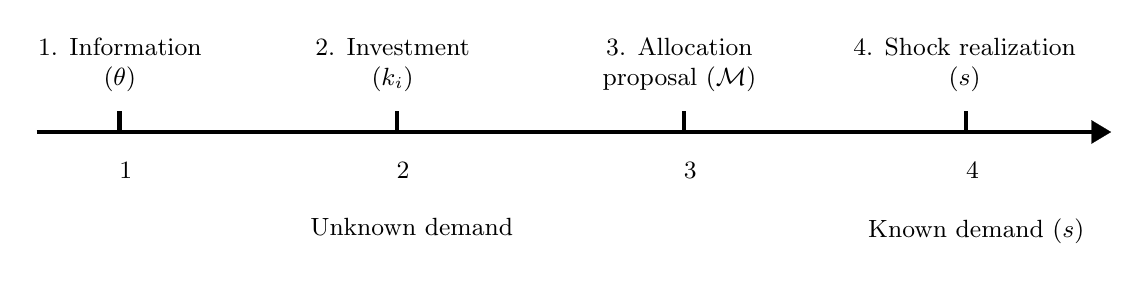
\begin{tikzpicture}[x=0.60pt,y=0.75pt,yscale=-1,xscale=1]

% Timeline line
\draw [line width=1.5] (20,100) -- (663,100);
\draw [shift={(667,100)}, rotate = 180.07] [fill=black][line width=0.08] (11.61,-5.58) -- (0,0) -- (11.61,5.58) -- cycle;

% Stage ticks
\foreach \x in {70,237,410,580} {
  \draw [line width=1.5] (\x,90) -- (\x,100);
}

% Stage labels
\draw (15,50) node [anchor=north west, font=\small, align=center] {1. Information \\ ($\theta$)};
\draw (182,50) node [anchor=north west, font=\small, align=center] {2. Investment \\ ($k_i$)};
\draw (355,50) node [anchor=north west, font=\small, align=center] {3. Allocation \\ proposal ($\mathcal{M}$)};
\draw (506,50) node [anchor=north west, font=\small, align=center] {4. Shock realization \\ ($s$)};

% Demand labels under line
\draw (179,137) node [anchor=north west, font=\small, align=center] {Unknown demand};
\draw (515,137) node [anchor=north west, font=\small, align=center] {Known demand ($s$)};

% Stage numbers under ticks
\draw (64,110) node [anchor=north west, font=\small] {1};
\draw (231,110) node [anchor=north west, font=\small] {2};
\draw (404,110) node [anchor=north west, font=\small] {3};
\draw (574,110) node [anchor=north west, font=\small] {4};

\end{tikzpicture}
\end{tcolorbox}
%%%%%%%%%%%%%%%%%%%%%%%%%%%%%%%%%%%%%%%%%%%%%%%%%%%%%%%%%%%%%%%%%%%%%%%%%%%%%%%%%%%%%%%%%%%%%%%%%%%%%%%%%%%%%%%%%%%%%%%%%%%%%%%%%%%%%%%%%%%%%%%%%%%%%%%%%%%%%%%%%%%%%%%%%%%%%%%%%%%%%%%%%%%%%%%%%%%%%%%%%%%%%%%%%%%%%%%%%%%%%%%%%%%%%%%%%%%%%%%%%%%%%%%%%%%%%%%%%%%%%%%%%%%%%%%%%%%%%%%%%%%%%%%%%%%%%%%%%%%%%%%%%%%%%%%%%%%%%%%%%%%%%%%%%%%%%%%%%%%%

\section{Complete Information Benchmark}\label{chap3sec:sec3}

The first regime we study is the complete information case: the market designer observes each consumer's type $\theta$ and welfare weight $\lambda$, so allocation rules can condition on true types without incentive issues. In this case, the original category label $i$ and the average weights $\tilde{\lambda}_i$ are uninformative for the market designer; allocations and transfers can be indexed directly by $(\theta,\lambda)$. Therefore, the market designer groups consumers according to their welfare weights. For tractability, we assume that the individual welfare weight $\lambda$ takes a finite number of values, denoted by $\{v_1,\ldots,v_{\tilde{n}}\}$.\footnote{Equivalently, the market designer discretizes the distribution of welfare weights.} For each $j\in \tilde N=\{1,\ldots,\tilde{n}\}$, the market designer defines a new category $j$ as the set of consumers whose weight equals $v_j$. Let $m_j$ be the total mass of consumers with weight $v_j$. Without loss of generality, we order the welfare weights as $0 < v_1 \leq \cdots \leq v_{\tilde{n}}$.

For each realization of the shock $s$, we define the allocation under complete information with $q^*_j(\theta, s)$ that maps the observed type of each consumer for each category to the quantity allocated. The monetary transfer $t^*_j(\theta,s)$ maps the observed type of each consumer to the payment made by the consumer to the market designer. We derive the optimization problem as follows, with the objective function corresponding to the weighted expected sum of consumer surpluses across types and states.

%%%%%%%%%%%%%%%%%%%%%%%%%%%%%%%%
\begin{align*}
\max_{\substack{ t_j(\theta,s) \geq 0, \\q_j(\theta,s) \geq 0}}  \quad \quad &  \sum_{j}  m_j  \; v_j  \; \E_{(s,\theta_j)} \left[\;\theta \; U(q_j(\theta,s),s)  -  t_j(\theta,s)\;\right] 
\end{align*}
%%%%%%%%%%%%%%%%%%%%%%%%%%%%%%%%

The allocation mechanism is budget-feasible and feasible if: the constraint \eqref{R-def} is satisfied (revenues must cover investment costs $I(k)$, given zero marginal production costs), the capacity constraint \eqref{K-def} is satisfied for all states $s$, and no consumer of every type $(\theta,j)$ has nonnegative expected utility as per the participation constraint \eqref{IR-def}. With multipliers $\varepsilon(s) \geq 0$ (capacity), $\beta\geq0$ (budget), $\rho_j\geq0$ (participation constraint), and $\phi_j(\theta,s)\geq 0$ (transfer positivity), the stationary conditions are 

\begin{align}
\label{KKT-q}\tag{FOC$_q^*$}
(m_jv_j+\rho_j)\;\theta \;u\!\left(q_j(\theta,s),s\right)\;-\;m_j\varepsilon(s) \;=\; 0,
\\
\label{KKT-t}\tag{FOC$_t^*$}
-m_jv_j + m_j\beta - \rho_j + \phi_j(\theta,s) \;=\; 0.
\end{align}

 We show in Lemma \ref{lemm1} that under a general mechanism, the optimal allocation is defined by a unique quantity schedule $q_j^*(\theta,s)$ and transfers are pinned down only at the category level. Let $s^*:= s^*(k)$ denote the first state in which the capacity constraint binds:
\[
\sum_{j} m_j \E_{\theta_j}q_j^*(\theta,s^*)\, dG_j(\theta) = k.
\]
We define $S^*=[\ubar{s},s^*)$ as the set of off-peak states (capacity slack) and $T^*=[s^*,\overline{s}]$ as the set of on-peak states (capacity binding). Let $U_j^*:= m_j\E_{(s,\theta_i)}[\theta U(q_j^*,s)]$ be the aggregate expected utility of category $j$ under the optimal allocation schedule. Define the cumulative sum $\mathbb{U}_m :=  \sum_{j=1}^m U_j$. The marginal category $j^*$ associated with the investment cost $I(k)$ is such that $\mathbb{U}_{j^*-1}<I(k) \leq \mathbb{U}_{j^*}$, then

%%%%%%%%%%%%%%%%%%%%%%%%%%%%%%%%
\begin{lemma}\label{lemm1}
Under the weighted objective with category weights $(v_j)_{j\in \tilde N}$, the optimal allocation is characterized by a unique quantity schedule $q_j^*(\theta,s)$ for each category $j\in\tilde N$, type $\theta$, and state $s$.


\[
\label{eq:FB-S}\tag{FB-S}
\theta u\!\left(q_j^*(\theta,s),s\right)=0, 
\qquad s\in S^{\ast},
\]
and
\[
\label{eq:FB-T}\tag{FB-T}
\theta u\!\left(q_j^*(\theta,s),s\right)=
\begin{cases}
\varepsilon(s)/\beta, & \text{if } j\le j^{\ast},\\[6pt]
\varepsilon(s)/v_j, & \text{if } j> j^{\ast},
\end{cases}
\qquad s\in T^{\ast},
\]

where $\varepsilon(s)\ge 0$ and $\beta\ge 0$ are the Lagrange multipliers on the capacity and budget constraints, and $j^*$  denotes the marginal category with $\beta =  v_{j^*}$. Moreover, the optimal transfers are independent of $s$ are such that $t_j^*(\theta) > 0 $ $\forall j \leq j^*$ and $t_j^*(\theta) = 0$ $\forall j > j^*$.

\end{lemma}

\begin{proof}
See Appendix \ref{ch3app:Ap1}
\end{proof}

The results follow from the Lagrangian of the program XXXX and generalize the Boiteux-Steiner framework (see \cite{crew1995theory}) to redistributive weights. We derive the optimal allocation with uniform weight in the Online Appendix. Off-peak ($s\in S^*$), the optimal allocation reproduces marginal-cost pricing: $u(q_j^*(\theta,s),\theta,s)=0$ which ensures that quantity is allocated until each consumer’s marginal willingness to pay equals the marginal production cost. On-peak ($s\in T^*$) and with heterogeneous weights, the optimal allocation depends on the transfer rule: given a shadow value of the budget constraint $\beta$, the market design selects every category $j$ such that $v_j\leq\beta$ and sets transfers so their participation constraint binds (except maybe for the marginal category). Therefore, the marginal category $j^*$ denotes the highest-weight category among those from which revenue is raised. $\forall j\leq j^*$, all transfers are positive and $\forall j>j^*$, all transfers are null. It induces the following individual allocation rule. For the contributing categories, the capacity is allocated such that the marginal willingness to pay is equal across all consumers: $u(q_j^*(\theta,s),\theta,s)=\varepsilon(s)/\beta$. If the market designer chooses to raise more revenue from category $j<j^*$, it needs to increase its allocation to relax the participation constraint, which is not the case for category $j^*$. The distortion in the allocation of $j$ implies that the market designer equalizes the marginal willingness to pay across those categories. For the non-contributing categories, the marginal willingness to pay is equal to the shadow value of the capacity $\varepsilon(s)$ scaled by the category weight $v_j$ and consumers with the higher weights receive a higher share of the capacity: for a given $\theta$ and if $v_j>v_j$, then $q^*_j(\theta,s) > q^*_j(\theta,s)$, since the marginal willingness to pay is strictly decreasing in $q$.

The direct implication is that a spot market does not implement the optimal allocation compared to the case with uniform weight $v_j$. Indeed, with only a spot market as the allocation mechanism, marginal utility is equal across consumers, violating the optimal condition for non-contributing categories. This stands in opposition to uniform $v_j$, as the optimal allocation requires that marginal utilities be equal across consumers, regardless of whether their IRs are slack or not. We formally describe the uniform case in the Online Appendix. \footnote{A mechanism that implements the optimal allocation with heterogeneous weight could consist of individualized two-part tariffs $(p_j,\Phi_j(\theta))$ with $p_j$ the unit price and $\Phi_j(\theta)$ the fixed part. The unit price would be uniform for the contributing categories. For the non-contributing category, the unit price varies across categories but is the same for every consumer within a category. The fixed part depends on both the category and the type $\theta$ to ensure IR. It is positive for contributing categories to extract the surplus and negative for non-contributing categories to ensure a null transfer.}  

Without additional structure, the sign of $\frac{\partial q_j}{\partial k}$ when the capacity is binding is generally ambiguous,\footnote{From equation \ref{eq:FB-S}, it is trivial that $k_i$ does not change the optimal allocation during off-peak states.} which limits the analysis of surplus changes. We derive sufficient conditions in the following Proposition for the increase in $k_i$ to lead to an increase in consumer surplus. To do so, for each category, define the weights that scale the marginal utility to $\varepsilon(s)$, the shadow value of a capacity at the optimum: $w^{nb}_j := - 1/(v_j u_q(q_j,\theta,s))$, for non-contributing categories, $w^{b}_j := -1/(\beta\,u_q(q_j,\theta,s))$ for contributing categories, as well the aggregate category weights $\overline{w}^{nb}$, $\overline{w}^{b}$ and $\overline{w}=\overline{w}^{b}+\overline{w}^{nb}$. The weights are positive since $u_q<0$. Then, define the weighted expected marginal utility over on-peak periods of contributing categories as
  
  \[\E_w[u]:=\E_s\left[ \sum_{j \leq j^*} m_j \E_{\theta_j}\left[\frac{w_j^b}{\overline{w}} \; \theta \; u(q_j^*(\theta,s),s))\right] \mathbf{1}_{s\in T^*}\right] \] 

then for any $s \in T^*$

\begin{proposition} 

\textbf{i)} For any interval $K\subseteq \mathbb{R}_+$ such that $j^*$ is constant for all $k\in K $ and the IR constraint of $j^*$ is slack then $U_j^*$ is (weakly) increasing in $k_i$ for all $j>j^*$. $U_{j^*}^*$ is (weakly) increasing in $k_i$ if and only if 
\[\E_w[u]\geq I'(k)\label{Ui*}\tag{Ui*}\]
  
\textbf{ii)} If $j^*$ has a binding IR and \eqref{Ui*} holds then ${U}_j$ is  (weakly) increasing in $k_i$ for all $j>j^*$.
\end{proposition}

The effect of a change of $k_i$ depends on whether the marginal category $j^*$ IR constraint is slack when $k_i$ changes. From equation \ref{eq:FB-T}, the optimal allocation for $j> j^*$ only depends on the shadow value of the capacity $\varepsilon(s)$: if an additional capacity always relaxes the optimal allocation ($\frac{\partial \varepsilon(s)}{\partial k}<0$), then optimal allocation of the non-contributing categories always increases, which also raises their surplus. For the marginal category, its surplus is relevant only when its IR constraint is slack. Its surplus corresponds to the residual budget once all contributing categories have exhausted their capacity constraints (i.e. $I(k) - \mathbb{U}_{j^*-1}^*$)

The case $i)$ Lemma relies on the optimality conditions that require $\beta = v_{j^*}$  for a given $k_i$; if the marginal category identity remains the same when $k_i$ changes, then $\partial_k \beta = 0$ and $\frac{\partial \varepsilon(s)}{\partial k}<0$. As the level of investment increases, the market designer does not need to distort the allocation of any category to relax the IR constraints of contributing categories. Therefore, the surplus increases for all non-contributing categories, and only for the marginal category if its marginal utility gain is higher than the marginal residual budget requirement.\footnote{The condition in the Lemma can be compared to the condition that gives the optimal investment level $k^*$ derived in the Online Appendix. Let's note the size $\mu^b=\sum_{j\leq j^*} m_j$ of the category having a positive transfer, then $k^*$ solves: 

\[\E_s\left[ \sum_{j \leq j^*} m_j \E_{\theta_j}\left[\frac{1}{\mu^b} \theta \; u(q_j^*(\theta,s),s))\right] \mathbf{1}_{s\in T^*}\right ]  = I'(k^*) \] 

Note that $1/\mu^b \geq 1 \geq \overline{w}_j^b/\overline{w}$. Therefore, if the left-hand parts of the two conditions are decreasing (which is a necessary condition for a unique optimal investment $k_i$ and that any category can be marginal only on a single interval), then an optimal investment level implies that the surplus of the marginal consumer is decreasing in $k_i$. The two conditions coincide when all categories are contributing (i.e., $\mu^b =1$ and $\overline{w}_j^b=\overline{w}$). In that case, this also corresponds to the optimal investment condition with uniform weights.

} Case $ii)$ assume that the IR constraint is binding for the marginal category and $\partial_k \beta \neq0$. Then, having the expected weighted utility greater than the marginal investment cost is a sufficient condition such that $\frac{\partial q_j}{\partial k}$ is positive for non-contributing categories. It has a direct interpretation: if the inequality \eqref{Ui*} holds, then the marginal benefit of an increase of capacity in terms of the (weighted) welfare of contributing categories is higher than the marginal cost of investment. Therefore, the market designer can self-finance the increase in additional capacity from the contributing category again without distorting their allocation ($\partial_k \beta < 0$). It induces that$\frac{\partial \varepsilon(s)}{\partial k}$ and $\partial_k q^*_j(\theta,s)>0$ for non-contributing category.

Condition \eqref{Ui*} is satisfied under two polar cases. For instance if either a) if the investment cost is constant in $k_i$ ($I'(k)=0$), or b) the utility follows the linear specification ($u_{qq} = 0$ and $u_{q\theta}=0$), $I'(0)=0$ and all categories have a binding IR ($j^*= n$). In terms of investment level, this holds for case $a)$ for all $k\in \mathbb{R}_+ $, and there exists $\overline{k}>0$ such that it holds on $[0,\overline{k})$ in case $b)$.\footnote{The first polar case is straightforward as if $I(k)$ is fixed then an increase in $k_i$ always free allocations. The second case is a sufficient condition that $\E_w[u]$ is decreasing in $k_i$, which ensures that condition \eqref{Ui*} may be satisfied for sufficient low $k_i$.}

We conclude in the following corollary the effect of a change in the weight distribution. 

\begin{corollary}

Consider a change in social weights $v_j$ such that for a given $k_i$: $j^*$ remains the marginal category, $dv_j<0$ for all $j<j^*$, $dv_{j^*}=0$, $dv_j>0$ for all $j>j^*$ and $\sum_j dv_j = 0$. Then, if $u$ is linear in $q$, condition \eqref{Ui*} becomes less stringent.

\end{corollary}

The results relies on decreasing the social weights of contributing categories towards non-contributing categories while holding the identity of the marginal category fix. It states that the condition, such that an increase in $k_i$ leads to a higher surplus for categories with slack IR, is less stringent when the non-contributing categories have higher social weight. The change of social weight decreases the quantity allocated to contributing categories, which raises their marginal utility: the marginal welfare gain from an increase in $k_i$ is therefore higher \textit{ceteris paribus}. It also lowers the aggregate weight $\overline{w}$ as contributing categories become more socially valuable.  

\section{Optimal allocation with private information}\label{chap3sec:sec5}

\subsection{Characterization}

We now assume that the consumer type is private information, while the consumer's category remains known to the market designer. In this framework, the direct mechanism consists of consumers reporting their type $\theta$. The mechanism assigns to each consumer of each category a quantity schedule $q^\times_i(\theta,s)$ and a transfer $t^\times_i(\theta,s)$. For private information, the mechanism is feasible if it satisfies the previous constraints \eqref{R-def}, \eqref{K-def}, and \eqref{IR-def}, as well as an incentive-compatibility constraint. That is, each agent reports its type truthfully if the following constraint is satisfied:

\[
\E_s[\theta U(q^\times_i(\theta,s),s)-t^\times_i(\theta,s)] \geq \E_s[\theta U(q^\times_i(\hat{\theta},s),s)-t^\times_i(\hat{\theta},s)]  \quad \quad \forall i,\theta,\hat{\theta}  \tag{IC}\label{IC-def}
\]

Constraint \eqref{IC-def} imposes incentive compatibility in expectation over $s$. In general, this only requires monotonicity of the expected marginal payoff from reporting truthfully, and it does not, by itself, imply that $\theta\mapsto q_i^\times(\theta,s)$ is nondecreasing for every state $s$. In our environment, however, the off-peak allocation will be independent of $\theta$, and on-peak allocations will be characterized by a first-order condition in which the dependence on $\theta$ enters through a term that does not vary with $s$. As a result, any potential failure of monotonicity (and any associated ironing) occurs across all peak states. Hence, for the purpose of the characterization, it is without loss to state monotonicity directly at the level of $q_i^\times(\theta,s)$ (rather than at the level of its expectation over $s$): if the allocation is monotone in $\theta$ in one peak state, it is monotone in all peak states, and the IC constraint \eqref{IC-def} is then satisfied. Additionally, under \eqref{IC-def}, transfers $t_i^\times(\theta,s)$ can be chosen so that, for each category $i$ and each type $\theta$, the  expected surplus satisfies, for some boundary term 
$\E\underline{CS}_i^\times \in \Big[0,\E_s\big[\underline{\theta}_i U(q^\times_i(\underline{\theta}_i,s),s)\big]\Big]$,

\[\tag{IC$^\times$}\label{ICmd-def}
\E CS_i^\times(\theta):=\E_s\!\left[\theta U\!\left(q_i^\times(\theta,s),s\right)-t_i^\times(\theta,s)\right]
= \E\underline{CS}_i^\times+\int_{\underline{\theta}_i}^{\theta}\E_s\!\left[U\!\left(q_i^\times(\tilde{\theta},s),s\right)\right]\,d\tilde{\theta}.
\]

This representation follows from standard envelope arguments; see \cite{milgrom2002envelope}. Let $\gamma_i(\theta)$ denote the inverse hazard rate of $G_i$ and $J_i(\theta)$ the virtual surplus function associated with a consumer from category $i$ and type $\theta$

\[\gamma_i(\theta):= \frac{1-G_i(\theta)}{g_i(\theta)} \quad \text{and} \quad  J_i(\theta):=\theta - \gamma_i(\theta)\]

Then define $\Lambda_i(\theta)$ is the $\lambda$-weighted mass of types above $\theta$ such that  $\Lambda_i(\theta)= \gamma_i(\theta) \E[ \ \lambda_i(\tilde \theta) \ | \ \tilde \theta \ \ge \ \theta \ ]$. The following lemma shows how the objective function can be represented

\begin{lemma}
The program of the market designer can be expressed as: 
\begin{align*}
\max_{q_i^\times(\theta,s), \, \E\underline{CS}_i^\times}  \quad\quad 
&  \sum_{i \in N}  \mu_i   \; 
\Big\{ \;  \tilde{\lambda}_i \;\E\underline{CS}_i^\times 
      + \E_{(s,\theta_i)} \big[\; \Lambda_i(\theta)\;  U(q_i^\times(\theta,s),s)\; \big] \;  \Big\}
\tag{CS$^\times$}\label{CSmd-def}  \\
\text{s.t.} \quad
& \sum_{i\in N}\mu_i
(\E_{(s,\theta_i)}\left[ U(q_i^\times(\theta,s),s) J_i(\theta) \right] - \E\underline{CS}_i^\times)\;-\; I(k)
\;\ge\; 0. \tag{R$^\times$}\label{Rmd-def}
\end{align*}
with the same capacity constraint \eqref{K-def} given allocation schedule $q_i^\times(\theta,s)$ and the participation constraint for the lower type,
$\E\underline{CS}_i^\times \in \Big[0,\E_s\big[\underline{\theta}_i U(q^\times_i(\underline{\theta}_i,s),s)\big]\Big]$ for all $i$.
\end{lemma}

The formulation of this new program stems from the separation of the transfer problem (the choice of $t^\times_i(\theta,s)$) from the allocation problem (the choice of $q^\times_i(\theta,s)$). Consider the case in which either the budget constraint or the IR constraint is binding while the other constraint is slack; then, a feasible lump-sum transfer from the non-binding constraint exists that allows relaxing the binding constraint while maintaining the other constraint slack. Such lump-sum transfers are defined in Lemma 2. They are conditioned by the IC/IR constraint, such that high types do not mimic low types, i.e., the market designer is constrained to finance the investment on the utility of the allocation net of the informational rent a consumer receives, and the lowest type derives non-negative utility from participating in the mechanism (see  \cite{Myerson1981,Ledyard2007})

Because the objective and all constraints are separable across categories $i$ except through the aggregate constraints
$\sum_i \mu_i k_i = k$ and $\sum_i \mu_i I_i = I(k)$, the designer problem can be decomposed into:
(i) an across-category allocation of $(k_i,I_i)$ subject to the two aggregate constraints, and
(ii) for each $i$, a within-category mechanism that chooses $\{q_i^\times(\theta,s)\}_{(\theta,s)}$ to respect capacity $k_i$ and raise revenue $I_i$.

\subsection{Optimal within-category allocation}\label{sec:within}

This section proceeds in four steps. First, we characterize the optimal allocation, which depends on whether the participation constraint binds. Second, we identify a sufficient statistic that governs the main results of the section and establish when its sign is single-crossing in $k_i$. Third, we analyze the individual welfare effects of capacity expansion and the conditions for implementing the optimal allocation. Finally, we examine how changes in redistributive preferences shape the optimal allocation.

%------------------------------------------------------------
\subsubsection{Characterization}
%------------------------------------------------------------

Following Lemma~\ref{CSmd-def}, the within-category problem selects an allocation rule $q_i^\times(\theta,s)$ to maximize category $i$'s contribution to the designer's objective, subject to a category-specific capacity level $k_i$ and revenue requirement $I_i$. Since transfers enter consumer surplus with a negative sign, any slack in the revenue requirement $(R_i^\times)$ could be rebated lump-sum to consumers while preserving incentive compatibility, raising the objective. Therefore the revenue requirement binds at the optimum: $\mathbb{E}_{(s,\theta_i)}[t_i^\times(\theta,s)] = I_i$. Substituting the envelope representation $(IC^\times)$ into this equality and integrating by parts with respect to $\theta$ — using the definition of $\gamma_i(\theta)$ and applying Lemma~\ref{CSmd-def} to separate the lump-sum transfer $\underline{CS}_i^\times$ from the allocation-dependent rent — yields the single combined constraint
\[
\E \underline{CS}_i^\times
=
\E_{(s,\theta_i)}\!\left[U\!\left(q_i^\times(\theta,s),s\right) J_i(\theta)\right]-I_i.
\tag{$\E \underline{CS}_i^\times$}\label{ECSi}\]
This reformulation combines the participation and budget requirements in a single constraint when the designer maximizes consumer surplus. Substituting $\E \underline{CS}_i^\times$ into the objective, the within-category problem becomes
\begin{align*}
\max_{q_i^\times(\theta,s)} \quad & \E_{(s,\theta_i)}\!\left[\Gamma_i(\theta)\,U\!\left(q_i^\times(\theta,s),s\right)-\tilde\lambda_i I_i\right]
\label{CSmdi-def}\tag{CS$^\times$} \\
\text{s.t.}\quad &
\E_{(s,\theta_i)}\!\left[U\!\left(q_i^\times(\theta,s),s\right) J_i(\theta)\right]-I_i \ge 0,
\label{Rmdi-def}\tag{IR-R$^\times_i$} \\
& \E_{\theta_i}\!\left[q_i^\times(\theta,s)\right]\le k_i \qquad \forall s.
\label{Kmdi-def}\tag{K$^\times_i$}
\end{align*}
Where
\[
\Gamma_i(\theta)=\tilde\lambda_i J_i(\theta)+\Lambda_i(\theta)
\]
captures the trade-off created by incentive constraints: reallocating $q$ toward type $\theta$ affects (i) revenue, proxied by the ``virtual surplus'' term $\tilde\lambda_i J_i(\theta)$, and (ii) surplus for types above $\theta$ through $\Lambda_i(\theta)$. Let $\varepsilon_i^\times(s)\ge 0$ and $\beta_i^\times\ge 0$ denote the multipliers on the capacity constraint \eqref{Kmdi-def} and the IR/budget constraint \eqref{Rmdi-def}. 





The first-order condition is
\[
\label{KKT-qMD}\tag{FOC$_q^\times$}
u\!\left(q_i^\times(\theta,s),s\right)\,\mathcal G_i(\theta)-\varepsilon_i^\times(s)=0,
\]
where $\mathcal G_i(\theta):=\Gamma_i(\theta)+J_i(\theta)\,\beta_i^\times$. We focus on interior solutions (i.e., all types receive a strictly positive allocation at the optimum):

\begin{assumption}\label{ass:interior}
For all $\theta\in\left[\underline{\theta}_i,\overline{\theta}_i\right]$, $\mathcal G_i(\theta)>0$ and $\Gamma_i(\theta)$ is non-decreasing in $\theta$, so that the monotonicity constraint on $q^\times_i(\theta,s)$ is satisfied at the optimum.\footnote{If this condition fails, standard Myerson-style ironing restores monotonicity without affecting the subsequent comparative statics, since the ironed weight $\overline{G}_i(\theta)$ enters the FOC in place of $\Gamma_i(\theta)$ but does not alter the structure of \eqref{Eujmd}. This stands in contrast with settings where the supply side imposes additional structure on the allocation: either indivisibility, as in \cite{CONDORELLI2013582}, or a fixed-quality schedule, as in \cite{akbarpour2023redistributive}, which restricts the set of implementable mechanisms.}
\end{assumption}

Define $S_i^\times=[\underline s,s_i^\times)$ and $T_i^\times=[s_i^\times,\overline s]$ as the off-peak and on-peak sets under the optimal allocation, where $s_i^\times$ satisfies $\E_{\theta_i}\!\left[q_i^\times(\theta,s_i^\times)\right]=k_i$.

\begin{lemma}\label{lem:FOC}
i) Under the weighted objective with type-dependent weights $\lambda(\theta)$, the allocation is characterized by a unique quantity schedule $q_i^\times(\theta,s)$ for each $\theta$ and $s$:
\[
\label{eq:SB-Smd1}\tag{SB-S}
u\!\left(q_i^\times(\theta,s),s\right)=0
\quad s\in S_i^\times,
\qquad \text{and} \qquad
u\!\left(q_i^\times(\theta,s),s\right)\,\G_i(\theta)=\varepsilon_i^\times(s)
\quad s\in T_i^\times.
\]
ii) If \eqref{Rmdi-def} is slack at $(k_i,I_i)$, then $\beta_i^\times=0$ and $\G_i(\theta)\equiv \Gamma_i(\theta)$.
\end{lemma}
%------------------------------------------------------------
\subsubsection{A sufficient statistic}\label{sec:suffstat}
%------------------------------------------------------------

The optimal allocation depends crucially on whether the capacity and participation constraints are binding. Before analysing the welfare effects and the implementation region, we identify a sufficient statistic that governs both. For notational simplicity, we suppress the dependence on $s$ and define
\[
  R_q(\theta) := -\frac{u\!\left(q_i^\times(\theta,s),s\right)}{u_q\!\left(q_i^\times(\theta,s),s\right)}, \qquad R_\theta(\theta) := \frac{J_i(\theta)}{\mathcal{G}_i(\theta)}. 
\]
Note that $R_q(\theta)\geq0$ since $u_q<0$. The term $R_q(\theta)$ governs how a marginal increase in $k_i$ is distributed across types at the optimal allocation: if $R_q(\theta)$ is decreasing in $\theta$, then, as capacity expands, a lower $\theta$ receives a higher share of the capacity than a higher $\theta$. $R_\theta(\theta)$ governs how marginal virtual surplus varies across types at the optimum: if $R_\theta(\theta)$ is increasing in $\theta$, then the marginal virtual surplus $u(q_i^\times,s)J_i(\theta)$ tends to be lower for lower types. Define the weights
\[
  w_i^\times(\theta,s):=-\frac{1}{u_q\!\left(q_i^\times(\theta,s),s\right)\mathcal{G}_i(\theta)}, \qquad \bar w_i^\times(s):=\mathbb{E}_{\theta_i}\!\left[w_i^\times(\theta,s)\right],
\]
and the $w_i^\times$-weighted average of the marginal virtual surplus
\begin{equation}
  \mathbb{E}_{w_i}[uJ\mid s] :=\frac{1}{\bar w_i^\times(s)} \mathbb{E}_{\theta_i}\!\left[w_i^\times(\theta,s)\, u\!\left(q_i^\times(\theta,s),s\right)J_i(\theta)\right] =\frac{1}{\bar w_i^\times(s)} \mathbb{E}_{\theta_i}\!\left[R_\theta(\theta)R_q(\theta)\right]. \tag{EuJ}\label{Eujmd}
\end{equation}
Therefore the signs of both expressions coincide. The following lemma establishes that this weighted average marginal virtual surplus is the sufficient statistic that simultaneously governs the revenue effect of capacity expansion, the sign of the budget multiplier, and the marginal change in the optimal allocation.

\begin{lemma}\label{lem:suffstat}
  The sign of\, \eqref{Eujmd} simultaneously determines:
  \begin{enumerate}[label=(\roman*), leftmargin=1cm]
    \item the sign of $\partial\mathbb{E}\underline{CS}_i^\times/\partial k_i$;
    \item the sign of $\partial\beta_i^\times/\partial k_i$ on the IR-constrained region;
    \item the direction of reallocation $\partial q_i^\times(\theta,s)/\partial k_i$.
  \end{enumerate}
  \end{lemma}

In particular, those objects governs the marginal welfare and redistributive aspect of a capacity extension (in Theorem~\ref{thm:welfare}) the feasibility of the optimal allocation (Proposition~\ref{prop:implementation}).

\eqref{Eujmd} depends on two dimensions: (i)~how the additional capacity is shared between types, captured by $R_q(\theta)$, and (ii)~how the marginal virtual surplus changes across types, captured by $R_\theta(\theta)$. The interaction between these two dimensions is formalised by the following condition:
\begin{equation}
  \mathbb{E}_{\theta_i}\!\left[R_\theta(\theta)R_q(\theta)\right] = \mathbb{E}_{\theta_i}[R_\theta(\theta)]\,\mathbb{E}_{\theta_i}[R_q(\theta)] + \operatorname{Cov}_{\theta_i}\!\left(R_\theta(\theta),R_q(\theta)\right) \geq 0. \tag{$\operatorname{COV}_{q\theta}^\times$}\label{COV1}
\end{equation}
The covariance term captures the \textit{capacity sorting effect}: it is adverse when the covariance in \eqref{COV1} is negative. For instance, if $R_q(\theta)$ is decreasing and $R_\theta(\theta)$ is increasing, then the lowest marginal virtual surplus is concentrated at the lowest $\theta$. In other words, as $k_i$ increases, a greater weight is placed on types with a potentially negative marginal virtual surplus. A decreasing virtual surplus ($J_i(\theta)<0$) implies that increasing $k_i$ reduces the budget the market designer can raise from those consumers. Therefore, the condition highlights the fundamental trade-off the market designer faces: increasing the allocation of a type, given its social weight, may conflict with revenue maximisation due to the IC constraint on higher types.

Lemma~\ref{lem:SC-dir} then provides mild monotonicity conditions under which this statistic is single-crossing in \(k_i\), so its sign---and therefore the qualitative predictions of the theorem and the implementation region---can be characterized sharply. The key primitive is whether the capacity sorting is \textit{submodular}: capacity expansion disproportionately benefits lower types.

\begin{definition}
  $R_q$ is \emph{submodular in $(\theta,k_i)$} if $\partial^2 R_q/\partial\theta\,\partial k_i\leq 0$
\end{definition}

\begin{lemma}[Single-crossing]\label{lem:SC-dir}
Assume \(R_\theta(\theta)\) is monotone in \(\theta\) and \(R_q(\theta,k_i)\) has monotone differences in \((\theta,k_i)\) (i.e., it is either submodular or supermodular).
Then the map
\[
k_i \longmapsto \mathbb E_{\theta_i}\!\left[R_\theta(\theta)\,R_q(\theta)\right]
\]
is single-crossing. Moreover, the direction is pinned down by the combination of monotonicities:
it crosses from \(+\) to \(-\) when \(R_\theta\) is increasing and \(R_q\) is submodular, or when \(R_\theta\) is decreasing and \(R_q\) is supermodular; it crosses from \(-\) to \(+\) in the two remaining cases.
\end{lemma}

The economic interpretation of monotone differences in $(\theta,k_i)$ is intuitive. Assume that $R_\theta(\theta)$ is increasing to higher types gets higher virtual surplus and $R_q(\theta)$ is submodular. When capacity is scarce, the designer allocates relatively uniformly across types; as $k_i$ expands, the incentive-compatible allocation is going disproportionately to lower types (as $R_q(\theta)$ increases more at the bottom). Combined with $R_\theta(\theta)$ increasing, the covariance term in \eqref{COV1} becomes increasingly negative as $k_i$ grows. At low capacity, the average effect $\mathbb{E}[R_\theta]\mathbb{E}[R_q]$ dominates and the sign of \eqref{Eujmd} is positive; at high capacity, the adverse sorting effect dominates and it becomes negative. Lemma~\ref{lem:SC-dir} formalises this single-crossing intuition.


\begin{remark}[Primitives for submodularity]\label{rem:prim}
We show in the proof of Lemma~\ref{lem:SC-dir} that the submodularity of $R_q$ in $(\theta,k_i)$ is equivalent to $R_q(\theta)$ being concave with respect to $q$:
\[
\frac{\partial^2 R_q(\theta)}{\partial \theta \partial k} \le 0 \quad\Leftrightarrow \quad \frac{\partial^2 R_q(\theta)}{\partial^2 q} \le 0.
\]
It is satisfied by standard utility specifications, including linear utility, exponential (CARA), power/isoelastic (CRRA), and, more generally, the HARA family.
\end{remark}

Moreover, we make the following assumptions throughout the section

\begin{assumption}\label{ass:monotone}
$R_q(\theta)$ and $R_\theta(\theta)$ are both monotone on $[\underline{\theta}_i,\overline{\theta}_i]$.
\end{assumption}

The monotonicity of $R_q(\theta)$ is used to interpret the sorting effect,\footnote{Note that due to the IC constraint, the monotocity of  $R_q(\theta)$ with respect to $\theta$ or $q$ is equivalent, as $\theta$ enter $R_q(\theta)$ only through $q$.} while the monotonicity of $R_\theta(\theta)$ is the key primitive for the welfare and implementation results that follow. Their signs depend on the model primitives as follows. For $R_q'(\theta)$, only the curvature of $u$ matters:
\[\sign\!\left(R_q'(\theta)\right)=-\sign\!\left((u_q(\cdot))^2-u(\cdot)u_{qq}(\cdot)\right),\]
so $R_q'(\theta)<0$ for linear and quadratic demand, while $R_q'(\theta)>0$ for CES/isoelastic demand. For $R_\theta'(\theta)$, the answer depends on whether the virtual surplus $J_i(\theta)$ grows faster or slower than the IC term $\Lambda_i(\theta)$ as $\theta$ increases,
\[
\label{signRt}\tag{$\sign R_\theta$}
\sign\!\left(R_\theta'(\theta)\right) = \sign\!\left(J_i(\theta)\right)\,\sign\!\Bigg(\underbrace{\frac{J_i'(\theta)}{J_i(\theta)}}_{\text{revenue term}} - \underbrace{\frac{\Lambda_i'(\theta)}{\Lambda_i(\theta)}}_{\text{IC term}}\Bigg).
\]
The first term flags whether a type contributes to revenue ($J_i(\theta)>0$) or not. The second compares the proportional growth rates of the two: when $\Lambda_i'(\theta)<0$, the IC term is shrinking, and the revenue term automatically dominates, giving $R_\theta'(\theta)>0$.\footnote{It is not possible to have a clear-cut sign of $R'_\theta(\theta)$. Indeed, the sign of $\Lambda_i'(\theta)$ depends on $g_i(\theta)$ and $\lambda_i(\theta)$: $\Lambda_i'(\theta)=-\Lambda_i(\theta)\frac{g_i'(\theta)}{g_i(\theta)}-\lambda_i(\theta)$. For instance, under a uniform distribution $\Lambda_i'(\theta)<0$, while its sign may be ambiguous for other distributions. Hence, under a uniform distribution, the sign of $R_\theta(\theta)$ is ambiguous as soon as $J_i(\theta)<0$. A utilitarian market designer (i.e., $\lambda_i(\theta)=G_i(\theta)$) does not imply a unique sign for $R_\theta(\theta)$, since it places implicit weight on higher types: in that case $\Gamma_i(\theta)=\theta$, and the IC term in \eqref{signRt} is positive (equal to $1/\theta$). If instead the correlation between types and social weights is zero, then the IC term is null and the sign of $R_\theta'(\theta)$ is determined solely by $J_i'(\theta)$, which is positive under regularity of $g_i(\theta)$.} 

\subsubsection{Welfare effects of $k_i$}\label{sec:welfare}
%------------------------------------------------------------

We now analyse how a marginal increase in $k_i$ is distributed across types in terms of individual surplus. A key insight is that this distribution does not depend directly on redistributive preferences: even when the designer places higher welfare weights on lower types, those types may still lose from capacity expansion. What governs the distribution of welfare gains is instead the sign of \eqref{Eujmd} identified in Lemma~\ref{lem:suffstat} together with the shape of $R_\theta(\theta)$. Redistributive preferences enter only indirectly, through their effect on the sign of \eqref{COV1} and on $R_\theta(\theta)$, as characterised in Section~\ref{sec:redist}.

The individual surplus change follows from \eqref{ICmd-def}:
\begin{equation}
  \frac{\partial\mathbb{E}CS_i^\times(\theta)}{\partial k_i} = \underbrace{\frac{\partial\mathbb{E}\underline{CS}_i^\times}{\partial k_i}}_{\text{boundary term}} +\underbrace{\int_{\underline\theta_i}^{\theta} \mathbb{E}_s\!\left[\frac{\partial q_i^\times(\tilde\theta,s)}{\partial k_i} u\!\left(q_i^\times(\tilde\theta,s),s\right)\right]d\tilde\theta}_{\text{IC rent}}. \tag{$\partial_k CS^\times$}\label{partialkCS1}
\end{equation}
To interpret both terms, we first record how the optimal allocation responds to a change in $k_i$. Differentiating the first-order condition \eqref{KKT-qMD} with respect to $k_i$ gives
\begin{equation}
  \frac{\partial q_i^\times(\theta,s)}{\partial k_i} = w_i^\times(\theta,s)\left( \frac{1}{\bar w_i^\times(s)} -\frac{\partial\beta_i^\times}{\partial k_i} \Bigl(\mathbb{E}_{w_i}[uJ\mid s] -u\!\left(q_i^\times(\theta,s),s\right)J_i(\theta)\Bigr) \right). \tag{$\partial_k q_i^\times$}\label{partialkq1}
\end{equation}
Using \eqref{Eujmd}, the boundary term can be decomposed as
\begin{equation}\label{partialkCS-boundary}
  \frac{\partial\mathbb{E}\underline{CS}_i^\times}{\partial k_i} = \mathbb{E}_s\Biggl[ \underbrace{\mathbb{E}_{\theta_i}\!\left[u(q_i^\times,s)J_i(\theta)\right]}_{\text{average effect}} + \underbrace{\operatorname{Cov}_{\theta_i}\!\left(u(q_i^\times,s)J_i(\theta)\,,\, \frac{\partial q_i^\times}{\partial k_i}\right)}_{\text{sorting effect}} \Biggr].
\end{equation}
Two observations about \eqref{partialkCS-boundary} are immediate. First, its sign is governed by \eqref{COV1}, as established in Lemma~\ref{lem:suffstat}. Second, when \eqref{Rmdi-def} binds (the IR-constrained allocation), the boundary term equals zero: the entire welfare change is then carried by the IC rent in \eqref{partialkCS1}.

\begin{theorem}\label{thm:welfare}
  Whenever it exists, define a cutoff $\tilde\theta_i\in [\underline\theta_i,\overline\theta_i]$ by $\partial\mathbb{E} CS_i^\times(\tilde\theta_i)/\partial k_i=0$.

  \medskip
  \noindent\textbf{IR-unconstrained allocation.} (i)~If \eqref{COV1} holds for every $s$, then an increase in $k_i$ increases surplus for every type $\theta$. (ii)~If \eqref{COV1} is reversed, then $\tilde\theta_i$ is unique; individual surplus decreases for all $\theta<\tilde\theta_i$ and increases for all $\theta>\tilde\theta_i$.

  \medskip
  \noindent\textbf{IR-constrained allocation} (characterised in Proposition~\ref{prop:implementation} below). Assume $R_\theta(\theta)$ is monotone. If $R_\theta(\theta)$ is increasing, then $\tilde\theta_i$ is unique and:
  \begin{enumerate}[label=(\roman*), leftmargin=1cm]
    \item if \eqref{COV1} holds for every $s$, individual surplus decreases for all $\theta>\tilde\theta_i$ and increases for all $\theta<\tilde\theta_i$;
    \item if \eqref{COV1} is reversed, individual surplus decreases for all $\theta<\tilde\theta_i$ and increases for all $\theta>\tilde\theta_i$.
  \end{enumerate}
  If $R_\theta(\theta)$ is decreasing, the inequalities are reversed.
\end{theorem}

Expanding capacity is not always surplus-improving for all consumers, even when the budget requirement does not bind (IR-unconstrained allocation) or for a fixed budget (IR-constrained allocation). Which types benefit from an increase in $k_i$ depends on two objects: (i)~the direction of the boundary term, governed by \eqref{COV1}, and (ii)~the shape of $R_\theta(\theta)$, which captures the trade-off between revenue extraction and incentive constraints.

When the participation constraint is slack ($\beta_i^\times=0$), the second term in parentheses in \eqref{partialkq1} vanishes, so the optimal allocation is increasing in $k_i$ for all types during on-peak states and constant off-peak. The boundary term in \eqref{partialkCS1} then corresponds to an equal change in surplus across all types, while the IC rent captures the additional incentive rents induced by the change in $q_i^\times$. If \eqref{COV1} holds, both terms are positive: the common component and the IC rent both increase with $k_i$, so an increase in $k_i$ improves the welfare of all consumers. If \eqref{COV1} is reversed, lower types are harmed. Indeed, the cross-partial derivative satisfies
\[
  \frac{\partial^2\mathbb{E}CS_i^\times(\theta)}{\partial k_i\,\partial\theta} =\mathbb{E}_s\!\left[\frac{\partial q_i^\times(\theta,s)}{\partial k_i} u\!\left(q_i^\times(\theta,s),s\right)\right],
\]
which is nonnegative in the IR-unconstrained allocation: the boundary term does not depend on $\theta$, while the marginal IC rent is increasing in $\theta$. This single-crossing property yields uniqueness of the cutoff in part~(ii), as well as the ordering of types that experience a decrease in surplus.

Under the IR-constrained allocation (i.e., when \eqref{Rmdi-def} binds), the allocation must be distorted so that expected revenue equals the budget. This distortion is captured by the second term in parentheses in \eqref{partialkq1}. We show in the proof that $\beta_i^\times$ is differentiable in $k_i$ on the IR-constrained region, and that the sign of $\partial\beta_i^\times/\partial k_i$ is governed by the sign of \eqref{Eujmd}, which is equivalently determined by \eqref{COV1}. The bracketed term in \eqref{partialkq1} is the deviation of a type's marginal virtual surplus $u(q_i^\times(\theta,s),s)J_i(\theta)$ from its $w_i^\times$-weighted average; its sign is therefore determined by the relative ranking of types according to marginal virtual surplus, which is captured by $R_\theta(\theta)$. If $R_\theta(\theta)$ is monotone, this deviation changes sign at most once, yielding a unique cutoff and the type-ranking described in Theorem~\ref{thm:welfare}. To interpret the condition, suppose expanding $k_i$ makes the budget less tight, so that $\beta_i^\times$ decreases in $k_i$. The need for revenue extraction then falls, and the designer lowers the marginal weight on types that generate higher marginal virtual surplus. The sign of $R_\theta(\theta)$ pins down which types those are.

The single-crossing result in Lemma~\ref{lem:SC-dir} has an immediate implication for the implementation regions of the optimal allocations: the capacity levels for which the IR-unconstrained allocation, and conversely the IR-constrained, is feasible and characterized by at most two thresholds.

\begin{proposition}[Implementation region]\label{prop:implementation}
Fix category \(i\) and a budget requirement \(I_i>0\). Let \(k_i^+\) be the capacity level at which the capacity constraint never binds. 
Assume that \eqref{Eujmd} is \emph{single-crossing in \(k_i\) from \(+\) to \(-\)} on \([0,k_i^+]\) for every $s$. Then \(\mathbb E\underline{CS}_i^\times(k_i)\) is single-peaked on \([0,k_i^+]\) and the set of capacities for which the IR-unconstrained allocation is feasible (equivalently, \(\mathbb E\underline{CS}_i^\times(k_i)\ge 0\)) has the following form:
\begin{enumerate}[label=(\roman*), leftmargin=1cm]
    \item If \(\mathbb E\underline{CS}_i^\times(k_i^+)\ge 0\), there exists a unique cutoff \(\tilde k_i\in(0,k_i^+]\) such that the IR-unconstrained allocation is optimal for all \(k_i\in[\tilde k_i,k_i^+]\). In particular, this holds whenever \(J_i(\theta)\ge 0\) for all \(\theta\).
    \item If \(\mathbb E\underline{CS}_i^\times(k_i^+)<0\), the IR-unconstrained allocation is either never optimal on \([0,k_i^+]\) or optimal only on an intermediate interval \([\tilde k_i^-,\tilde k_i^+]\subset(0,k_i^+)\).
\end{enumerate}

If instead \eqref{Eujmd} crosses from \(-\) to \(+\) for every $s$: then \(\mathbb E\underline{CS}_i^\times(k_i)\) is single-dipped on \([0,k_i^+]\) and either \(\mathbb E\underline{CS}_i^\times(k_i)<0\) for all \(k_i\in[0,k_i^+]\), or there exists a unique \(\tilde k_i\in(0,k_i^+]\) such that \(\mathbb E\underline{CS}_i^\times(k_i)\ge 0\) for all \(k_i\in[\tilde k_i,k_i^+]\).

\end{proposition}

The threshold $\tilde k_i$ defines when the market designer can finance the investment $I_i$ without distorting the allocation via the IR constraint. The condition follows directly from the single-crossing of $\mathbb{E}[uJ]$ in $k_i$ established in Lemma~\ref{lem:SC-dir}: as capacity expands and adverse sorting worsens, the expected revenue that the mechanism can sustain first increases and then falls. The intersection of this revenue curve with $I_i$ pins down the implementation threshold. In general, \eqref{COV1} does not hold pointwise in $s$: because of the capacity constraint, the optimal allocation varies with $s$, and the aggregate effect depends on how the virtual term $J_i(\theta)$ is sorted across types as $s$ changes.

Figure~\ref{fig:impl_welfare} synthesizes the joint implications of Lemma~\ref{lem:SC-dir}, Proposition~\ref{prop:implementation}, and Theorem~\ref{thm:welfare} under submodular $R_q$ and increasing $R_\theta(\theta)$. The capacity axis is partitioned into four regions by three thresholds: the two IR-regime boundaries $\tilde k_i^-$ and $\tilde k_i^+$ from Proposition~\ref{prop:implementation}, and the zero-crossing $k^\ast$ of \eqref{Eujmd} from Lemma~\ref{lem:SC-dir}. For low capacity levels $k_i \in [0, \tilde k_i^-)$, the IR constraint binds and \eqref{COV1} holds: only lower types benefit from capacity expansion, so the welfare effect is progressive. As capacity crosses $\tilde k_i^-$, the mechanism becomes IR-unconstrained and \eqref{COV1} still holds, so all types gain --- this is the universal region. The covariance reverses at $k^\ast$, still within the IR-unconstrained region: higher types now gain and lower types lose, so the welfare effect turns regressive. Finally, beyond $\tilde k_i^+$, the IR constraint binds again and the adverse sorting is sufficiently severe that only higher types continue to benefit. Two features of this picture are worth emphasizing. First, the welfare character --- who gains from $\uparrow k_i$ --- is governed entirely by the sign of \eqref{COV1}, which switches at $k^\ast$, not at the IR-regime boundaries. Second, under case (ii) of Proposition~\ref{prop:implementation}, the single-peakedness of \eqref{Eujmd} and its negative value at $k_i = 0$ jointly guarantee the ordering $\tilde k_i^- < k^\ast < \tilde k_i^+$, so all four regions are generically non-empty, with degenerate cases arising only when extreme segments collapse.
\begin{figure}[h]
\centering
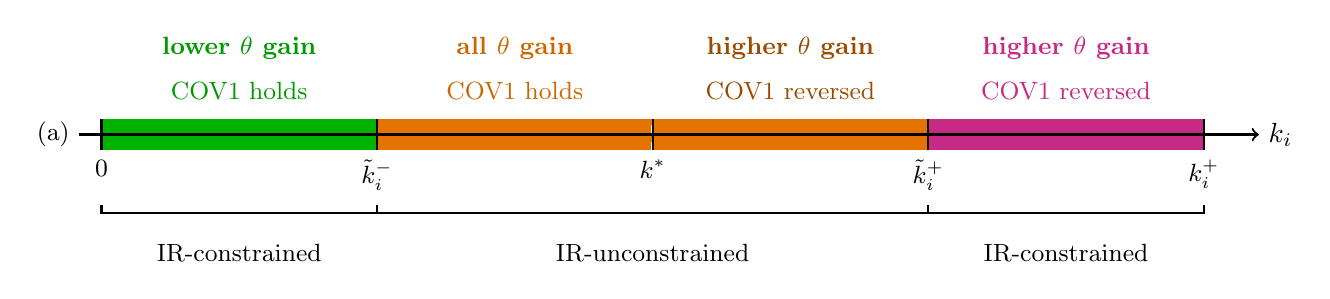
\begin{tikzpicture}[x=1.4cm, y=1cm]
\fill[green!70!black]   (0,   -0.2) rectangle (2.5,  0.2);
\fill[orange!90!black]  (2.5, -0.2) rectangle (5.0,  0.2);
\fill[orange!90!black]  (5.0, -0.2) rectangle (7.5,  0.2);
\fill[magenta!80!black] (7.5, -0.2) rectangle (10.0, 0.2);
\draw[white, dashed, line width=1pt] (5.0,-0.2) -- (5.0,0.2);
\draw[thick] (0,-0.9)   -- (0,-1.0)   -- (2.5,-1.0) -- (2.5,-0.9);
\draw[thick] (2.5,-0.9) -- (2.5,-1.0) -- (7.5,-1.0) -- (7.5,-0.9);
\draw[thick] (7.5,-0.9) -- (7.5,-1.0) -- (10,-1.0)  -- (10,-0.9);
\node[font=\small] at (1.25, -1.5)  {IR-constrained};
\node[font=\small] at (5.0,  -1.5)  {IR-unconstrained};
\node[font=\small] at (8.75, -1.5)  {IR-constrained};
\node[font=\small, green!60!black]   at (1.25, 0.55) {\eqref{COV1} holds};
\node[font=\small, orange!80!black]  at (3.75, 0.55) {\eqref{COV1} holds};
\node[font=\small, orange!60!black]  at (6.25, 0.55) {\eqref{COV1} reversed};
\node[font=\small, magenta!80!black] at (8.75, 0.55) {\eqref{COV1} reversed};
\node[font=\small\bfseries, green!60!black]   at (1.25, 1.1)  {lower $\theta$ gain};
\node[font=\small\bfseries, orange!80!black]  at (3.75, 1.1)  {all $\theta$ gain};
\node[font=\small\bfseries, orange!60!black]  at (6.25, 1.1)  {higher $\theta$ gain};
\node[font=\small\bfseries, magenta!80!black] at (8.75, 1.1)  {higher $\theta$ gain};
\draw[->, thick] (-0.2, 0) -- (10.5, 0);
\node[right] at (10.5, 0) {$k_i$};
\foreach \x/\lbl in {0/$0$, 2.5/$\tilde k_i^-$, 5/$k^\ast$, 7.5/$\tilde k_i^+$, 10/$k_i^+$}{
  \draw[thick] (\x, 0.2) -- (\x, -0.2);
  \node[below, font=\small] at (\x, -0.2) {\lbl};
}
\node[left, font=\small] at (-0.2, 0) {(a)};
\end{tikzpicture}

\vspace{1.2cm}

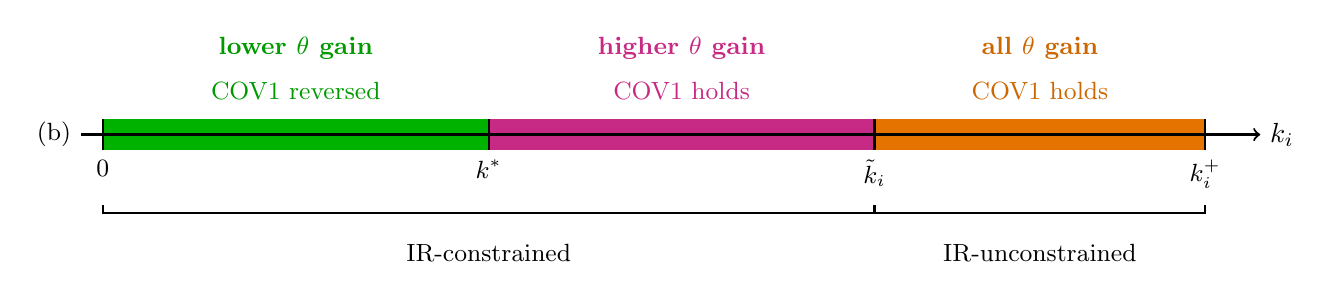
\begin{tikzpicture}[x=1.4cm, y=1cm]
\fill[green!70!black]   (0,   -0.2) rectangle (3.5,  0.2);
\fill[magenta!80!black] (3.5, -0.2) rectangle (7.0,  0.2);
\fill[orange!90!black]  (7.0, -0.2) rectangle (10.0, 0.2);
\draw[thick] (0,-0.9)   -- (0,-1.0)   -- (7.0,-1.0) -- (7.0,-0.9);
\draw[thick] (7.0,-0.9) -- (7.0,-1.0) -- (10,-1.0)  -- (10,-0.9);
\node[font=\small] at (3.5,  -1.5)  {IR-constrained};
\node[font=\small] at (8.5,  -1.5)  {IR-unconstrained};
\node[font=\small, green!60!black]   at (1.75, 0.55) {\eqref{COV1} reversed};
\node[font=\small, magenta!80!black] at (5.25, 0.55) {\eqref{COV1} holds};
\node[font=\small, orange!80!black]  at (8.5,  0.55) {\eqref{COV1} holds};
\node[font=\small\bfseries, green!60!black]   at (1.75, 1.1)  {lower $\theta$ gain};
\node[font=\small\bfseries, magenta!80!black] at (5.25, 1.1)  {higher $\theta$ gain};
\node[font=\small\bfseries, orange!80!black]  at (8.5,  1.1)  {all $\theta$ gain};
\draw[->, thick] (-0.2, 0) -- (10.5, 0);
\node[right] at (10.5, 0) {$k_i$};
\foreach \x/\lbl in {0/$0$, 3.5/$k^\ast$, 7.0/$\tilde k_i$, 10/$k_i^+$}{
  \draw[thick] (\x, 0.2) -- (\x, -0.2);
  \node[below, font=\small] at (\x, -0.2) {\lbl};
}
\node[left, font=\small] at (-0.2, 0) {(b)};
\end{tikzpicture}
\caption{Joint characterization of the implementation regime and welfare effects of capacity expansion. Panel (a): submodular $R_q$ and increasing $R_\theta(\theta)$, so \eqref{Eujmd} crosses from $+$ to $-$. Panel (b): supermodular $R_q$ and decreasing $R_\theta(\theta)$, so \eqref{Eujmd} crosses from $-$ to $+$. In both panels, the welfare character (who gains from an increase in $k_i$) is governed by the sign of \eqref{COV1}, independently of the IR regime.}
\label{fig:impl_welfare}
\end{figure}

The following corollary provides functional-form conditions under which the sign of \eqref{COV1} is independent of $(s,k_i)$. It isolates the distribution of virtual surplus $J_i(\theta)$ relative to social weights $\Gamma_i(\theta)$ as the sole determinant of the implementation region, confirming that the key primitive is how revenue generation is distributed across types rather than the level or state of the capacity allocation.

\begin{corollary}\label{cor:sep}
  Assume $u(q,s)$ is additively separable in $(q,s)$ and linear in $q$ and $s$. Then the sign of $\mathbb{E}_{\theta_i}[R_\theta(\theta)R_q(\theta)]$ equals the sign of
  \[
    \mathbb{E}_{\theta_i}\!\left[\frac{J_i(\theta)}{\mathcal{G}_i(\theta)^2}\right],
  \]
  which is independent of $s$ and $k_i$.
\end{corollary}

We illustrate in Figure~\ref{fig:redistribution_marg_k_uniform} the results from Theorem~\ref{thm:welfare} and Proposition~\ref{prop:implementation} as well as the the sensitivity of the implementation regions with respect to the model primitives. The first panel shows the value of the boundary term \eqref{ECSi} with respect to $k_i$ for two different types support. It represents both the implementation region of the optimal allocation as well as the regions of the sign of \eqref{COV1}. As a key element of this analysis is the existence of types with negative marginal virtual surplus, we show how an increase of the mass of such consumer affects the outcome of the model. To do so, the second support has a lower $\underline{\theta}_i$ which mechanically increase the mass of consumers having $J_i<0$. As expected this reduces the occurrence of capacity level for which the condition \eqref{COV1} is satisfied.\footnote{Intuitively, this reduces $k^\ast$ which reduces the progressivity of an increase of $k_i$ for lower types ($k^\ast$ on Figure~\ref{fig:impl_welfare} moves to the left).} The second panel with the set of plots illustrate how the progressivity/regressivity of the a capacity extension depends on the level of investment. The left panel shows 2 initial investment level ($k_1$ and $k_3$) and their respective deviation ($k_2$ and $k_4$). For initially low value ($k_1$) all consumers benefits from an increase in $k_i$ (when \eqref{COV1} is satisfied under the IR unconstrained), while for higher values of $k_i$ ($k_3$, when  \eqref{COV1} is not satisfied), lower types below the threshold $\tilde\theta_i$ experienced a loss of surplus while all type above increases their surplus.

We illustrate in Figure~\ref{fig:redistribution_marg_k_uniform} the results from Theorem~\ref{thm:welfare} and Proposition~\ref{prop:implementation} as well as the sensitivity of the implementation regions with respect to the model primitives. The first panel shows the value of the boundary term \eqref{ECSi} with respect to $k_i$ for two different type supports. It represents both the implementation region of the optimal allocation and the regions of the sign of \eqref{COV1}. Since a key element of this analysis is the existence of types with negative marginal virtual surplus, we show how an increase in the mass of such consumers affects the outcome of the model. To do so, the second support has a lower $\underline{\theta}_i$, which mechanically increases the mass of consumers having $J_i<0$. As expected, this reduces the range of capacity levels for which condition \eqref{COV1} is satisfied.\footnote{Intuitively, this reduces $k^\ast$, which reduces the progressivity of an increase of $k_i$ for lower types ($k^\ast$ on Figure~\ref{fig:impl_welfare} moves to the left).} The left panel also marks two initial investment levels ($k_1$ and $k_3$) and their respective deviations ($k_2$ and $k_4$), whose individual surplus effects are illustrated in the right panel. For an initially low value ($k_1$), all consumers benefit from an increase in $k_i$ when \eqref{COV1} is satisfied under the IR-unconstrained allocation, while for a higher value of $k_i$ ($k_3$), when \eqref{COV1} is reversed, lower types below the threshold $\tilde\theta_i$ experience a loss of surplus while all types above benefit. The figure focuses on the IR-unconstrained region of Theorem~\ref{thm:welfare}; the IR-constrained predictions and the single-threshold case of Proposition~\ref{prop:implementation} are qualitatively consistent with the same numerical example but are omitted for brevity.

\begin{figure}
\centering
\includegraphics[width=1\linewidth]{figure/redistribution_marg_k_uniform.png}
\caption{Illustration of the individual surplus effect of a capacity expansion. The illustration is based on a quadratic utility function $U(q,s)=(1+s)q - \tfrac{1}{4}q^2,$ with $J_i(\theta)$ derived from a uniform distribution of types, which implies an increasing $R_\theta(\theta)$, and the budget requirement set to $I_i = 0.45$.}
\label{fig:redistribution_marg_k_uniform}
\end{figure}

\subsubsection{Redistributive preferences and the optimal allocation}\label{sec:redist}
We now examine how changes in redistributive preferences affect the optimal allocation and the previous results. This comes through two channels. First, it directly changes the trade-off between revenue and incentive constraints, captured by $\Delta R_\theta(\theta)$ (we formally define below the preference-perturbation operator $\Delta(\cdot)$). Second, it induces a behavioral response in the optimal allocation $q_i^\times(\theta,s)$, which in turn changes $R_q$. We conclude the section with Corollary~\ref{cor:CARA}, which provides a specification of the utility function under which a change of preferences unambiguously impacts $\mathbb{E}_{\theta_i}[R_\theta(\theta)R_q(\theta)]$ and therefore \eqref{Eujmd}, since $\bar w_i^\times(s)>0$ for all $s$.


Formally, the total effect of a preference change on \eqref{COV1} decomposes as
\[
\Delta \E_{\theta_i}\!\left[R_\theta(\theta)R_q(\theta)\right]
=
\underbrace{\E_{\theta_i}\!\left[\Delta R_\theta(\theta)\,R_q(\theta)\right]}_{\text{trade-off effect}}
+
\underbrace{\E_{\theta_i}\!\left[R_\theta(\theta) \; \Delta R_q(\theta) \right]}_{\text{behavioral effect}},
\]
and since $R_q$ depends on the preferences only through $q_i^\times$, we have $\Delta R_q(\theta)=\frac{\partial R_q(\theta)}{\partial q}\,\Delta q_i^\times(\theta,s)$. Proposition~\ref{prop:rho-q-cov-iron2} provides conditions under which a change of preferences unambiguously impacts the trade-off channel. Proposition~\ref{prop:rprefreallocation} shows that $\Delta q_i^\times(\cdot,s)$ is generically non-monotone in $\theta$, even when the absolute weight change $\Delta\Gamma_i(\theta)$ is monotone. As a result, without further restrictions on preferences and demand curvature, the behavioral channel cannot be signed in general.

We now characterize the consequences of a (marginal) perturbation of preferences, denoted $\Delta\lambda_i(\theta)$. The induced change in the welfare weight is
\[
\Delta\Gamma_i(\theta)=J_i(\theta)\,\Delta\tilde\lambda_i+\Delta\Lambda_i(\theta),
\qquad \text{with} \qquad
\Delta\Lambda_i(\theta)=\gamma_i(\theta)\E\!\left[\Delta\lambda_i(\tilde\theta)\mid \tilde\theta\ge \theta\right].
\]

The following Lemma establishes the link between a particular change of redistributive preferences and the $\Delta\Gamma_i(\theta)$.

\begin{lemma}\label{lem:preferenceorder}
Consider a weight function $\lambda_i(\theta)$ and its perturbation
$\lambda_i^\Delta(\theta)$, with $\Delta\lambda_i(\theta)
:=\lambda_i^\Delta(\theta)-\lambda_i(\theta)$ and
$\Delta\Gamma_i(\theta):=\Gamma_i^\Delta(\theta)-\Gamma_i(\theta)$.
Suppose $\Gamma_i(\theta),\Gamma_i^\Delta(\theta)>0$ for all
$\theta\in[\underline{\theta}_i,\overline{\theta}_i]$. Then:

\noindent i) If $\lambda_i^\Delta(\theta)$ shifts preferences toward higher types proportionally more than $\lambda_i(\theta)$, in the sense that $\frac{\lambda_i^\Delta(\theta)}{\lambda_i(\theta)}$ is increasing on $[\underline{\theta}_i,\overline{\theta}_i]$; and $\tilde{\lambda}_i^\Delta\ge \tilde{\lambda}_i$,
        then for all $\theta\in[\underline{\theta}_i,\overline{\theta}_i]$,
        \[
          \frac{\Lambda_i^{\Delta\,\prime}(\theta)}{\Lambda_i^\Delta(\theta)}
          \;\ge\;
          \frac{\Lambda_i^{\prime}(\theta)}{\Lambda_i(\theta)},
          \qquad\text{and}\qquad
          \Delta\Gamma_i(\theta)\;\ge\;0.
        \]
\noindent ii) If $\lambda_i^\Delta(\theta)$ shifts preferences toward lower types proportionally more than $\lambda_i(\theta)$, in the sense that $\frac{\lambda_i^\Delta(\theta)}{\lambda_i(\theta)}$ is decreasing on $[\underline{\theta}_i,\overline{\theta}_i]$; and $\tilde{\lambda}_i^\Delta\le \tilde{\lambda}_i$,
        then for all $\theta\in[\underline{\theta}_i,\overline{\theta}_i]$, the inequalities reverse.
\end{lemma}

Lemma~\ref{lem:preferenceorder} thus connects the direction of a preference shift --- toward higher or lower types --- to the sign of $\Delta\Gamma_i(\theta)$: tilting welfare weights proportionally toward higher types, while not decreasing the average weight, raises social weights pointwise, and conversely.

It also has a direct implication for the sign of $R'_\theta(\theta)$. From expression \eqref{signRt}, only the IC term depends on preferences; the revenue term is determined solely by the type distribution. For instance, assume $\Lambda_i^{1\,\prime}(\theta)<0$, $\Lambda_i^{2\,\prime}(\theta)<0$, and $J_i'(\theta)>0$. In that case, a preference shift toward higher types favors $R_\theta'(\theta)>0$. For types generating revenue ($J_i(\theta)>0$), $R_\theta'(\theta)>0$ holds under both weight functions. For types that do not generate revenue ($J_i(\theta)<0$), $R_\theta'(\theta)>0$ requires $\Lambda_i'(\theta)/\Lambda_i(\theta)$ to be sufficiently close to zero; since $\Lambda_i^{\Delta\,\prime}/\Lambda_i^\Delta \ge \Lambda_i^{\prime}/\Lambda_i$ by Lemma~\ref{lem:preferenceorder}, this condition is easier to satisfy under a preference shift toward higher types.

Define the ratio
\[
R_\Gamma(\theta):=\frac{\Delta\Gamma_i(\theta)}{\Gamma_i(\theta)}
\]
that captures the proportional change in preferences. The proposition below formalizes how a preference shift affects the trade-off effect. Write the trade-off effect as
\[
\E_{\theta_i}\!\left[\Delta R_\theta(\theta)\, R_q(\theta)\right]
=
\underbrace{\E_{\theta_i}\!\left[\Delta R_\theta(\theta)\right]}_\text{trade-off average effect}\,\E_{\theta_i}\!\left[R_q(\theta)\right]
+
\underbrace{\Cov_{\theta_i}\!\left(\Delta R_\theta(\theta),R_q(\theta)\right)}_\text{trade-off sorting effect},
\]
\begin{proposition}\label{prop:rho-q-cov-iron2}
Assume that both $R_\theta(\theta)$ and $R_q(\theta)$ are monotone and that $\Delta \Gamma_i(\theta)$ has a constant sign for all $\theta$. Suppose that the following two conditions hold:
\begin{enumerate}[label=(\roman*), leftmargin=1cm]
\item \emph{(Average effect condition)} $\mathrm{sign}\!\left(\mathbb{E}_{\theta_i}\!\left[\Delta R_\theta(\theta)\right]\right) = \mathrm{sign}\!\left(\mathrm{Cov}_{\theta_i}\!\left(\Delta R_\theta(\theta), R_q(\theta)\right)\right)$.
\item \emph{(Elasticity condition)} for all $\theta$:
\[\left|\frac{R_\Gamma'(\theta)}{R_\Gamma(\theta)}\right| \le  \left|\frac{R_\theta'(\theta)}{R_\theta(\theta)}\right|.\]
\end{enumerate}
Then, for any sign configuration of $(R_\Gamma(\theta), R_\theta'(\theta), R_q'(\theta))$ such that $\mathrm{sign}(-R_\Gamma(\theta)R_\theta'(\theta))$ aligns with the sign of $\Delta R_\theta'(\theta)$, \[\mathrm{sign}\!\left(\mathbb{E}_{\theta_i}\!\left[\Delta R_\theta(\theta)\, R_q(\theta)\right]\right) = \mathrm{sign}\!\left(-R_\Gamma(\theta) R_\theta'(\theta)\right) \cdot \mathrm{sign}\!\left(R_q'(\theta)\right).\] In sign configurations where $\mathrm{sign}(-R_\Gamma(\theta)R_\theta'(\theta))$ does not align with the sign of $\Delta R_\theta'(\theta)$, condition~(ii) is necessary but not sufficient to sign $\mathbb{E}_{\theta_i}\!\left[\Delta R_\theta(\theta)\, R_q(\theta)\right]$.
\end{proposition}

The proposition provides sufficient conditions under which a change in redistributive preferences unambiguously affects the trade-off covariance term. Condition~(i) ensures that the average effect has the correct sign and it cannot in general be derived from primitives since $R_\Gamma$ need not be monotone in $\theta$ and must therefore be imposed directly. Condition~(ii) is a uniform sufficient condition across all achievable sign configurations. It compares two elasticities: (i) $\left|\frac{R_\Gamma'(\theta)}{R_\Gamma(\theta)}\right|$, which measures how sharply the preference change varies across types, and (ii) $\left|\frac{R_\theta'(\theta)}{R_\theta(\theta)}\right|$, which measures how sharply the existing sorting pattern varies across types. The condition requires that the preference change be smoother in proportional terms than the existing sorting pattern. The sorting condition follows from differentiating $R_\theta(\theta)$: 
\[\Delta\!\left(R_\theta'(\theta)\right) = -R_\theta(\theta)\,R_\Gamma'(\theta)-R_\Gamma(\theta)\,R_\theta'(\theta).\] 
The proposition considers all possible case given any sign configuration of $(R_\Gamma(\theta), R_\theta'(\theta), R_q'(\theta))$.
To interpret its economic meaning, consider the case where lower types are allocated more capacity ($R_q'(\theta)\le 0$), higher types gets higher rents ($R'_\theta(\theta)\ge 0$), the change of preferences is towards higher types ($\Delta R_\Gamma\ge 0$), and we are looking to reduce the adverse sorting effect such that the covariance term is positive ($\Delta R_\theta'(\theta) \le 0 $). Then a change of preference ---even in the correct direction---can exacerbate adverse sorting by creating local distortions. More specifically, the sufficient elasticity condition binds in two regions: (a) types contributing negatively to the trade-off ($R_\theta(\theta)<0$) but receiving increasing proportional weights ($R_\Gamma'(\theta)\ge 0$), and (b) types contributing positively to the trade-off ($R_\theta(\theta)>0$) but receiving decreasing proportional weights ($R_\Gamma'(\theta)\le 0$). In both regions, preference changes that are too concentrated reverse the sign of $\Delta(R_\theta'(\theta))$; the elasticity bound ensures changes remain sufficiently gradual. 

We illustrate the implications of the proposition in Figure \ref{fig:variation_uniform_preference_tradeoff}: even when the direction of a preference shift favors the same consumers, particular concentration of social weights adjustments can exacerbate adverse sorting, worsening rather than improving the trade-off effect. The first plot represents two similar perturbations: from a utilitarian market designer where $\lambda_i(\theta) =1$ to a weight function that favors higher types (in both cases). The middle set of plots shows that the perturbation in the case A leads to a non monotonic change in $\Delta R_\theta(\theta)$ with respect to $\theta$, compared to case B, which is strictly decreasing (we assume that $R_q$ is decreasing in $\theta$). In case A, this increasing part of the function leads to a negative covariance. The right panel shows that the increasing part is due to the violation of the sufficient conditions in the Proposition.

\begin{figure}
    \centering
    \includegraphics[width=1\linewidth]{figure/variation_uniform_preference_tradeoff.png}
    \caption{Effects of change in redistributive preferences on the trade-off effect. The first plot shows the new $\lambda_i(\theta)$. The second plot indicates the effect of the perturbation on the term $\Delta R_\theta(\theta)$. The last plot links the condition in Proposition \ref{prop:rho-q-cov-iron2} to the sign of $\Delta R'_\theta(\theta)$. $R_q(\theta)$ is assumed to be decreasing in $\theta$, $R_\theta(\theta)$ and $J_i(\theta)$ are increasing in $\theta$. In this example, $R'_\Gamma(\theta)<0$ and $J_i(\theta)>0$ for all $\theta$, so the worsening effect comes from types generating revenues while receiving proportionally decreasing weights.}
    \label{fig:variation_uniform_preference_tradeoff}
\end{figure}

We conclude with the effect of preferences on the behavioral response, i.e., how a change in social weights affects the optimal allocation $q_i^\times(\theta,s)$.

\begin{proposition}\label{prop:rprefreallocation}
\noindent{\bf Preferences and reallocation.}
Fix a peak state $s\in T_i^\times$.

\noindent (A) If $R_\Gamma$ is not (a.e.) constant, then $\Delta q_i^\times(\cdot,s)$ is not monotone on $\Theta_i$.

\noindent  (B) Moreover, assume that $R_\Gamma(\theta)$ is unimodal and that $\Delta\lambda(\theta)$ is mean-preserving. Then there exist unique cutoffs $\theta_-<\theta_+$ solving $u(q_i^\times(\theta,s),s)\,\Delta\Gamma_i(\theta)=\Delta\varepsilon_i(s)$ such that:
(i) if $\Delta\Gamma_i(\theta)\ge 0$ for all $\theta$, then $\Delta q_i^\times(\theta)\le 0$ for $\theta\in[\underline\theta,\theta_-)\cup(\theta_+,\overline\theta]$ and $\Delta q_i^\times(\theta)\ge 0$ for $\theta\in[\theta_-,\theta_+]$;
(ii) if $\Delta\Gamma_i(\theta)\le 0$ for all $\theta$, the inequalities are reversed.
\end{proposition}

The first part of Proposition~\ref{prop:rprefreallocation} has strong consequences for the welfare analysis of preference shifts. Since the aggregate effect combines an average component and a sorting component, and since the behavioral response $\Delta q_i^\times(\cdot,s)$ is non-monotone in types, it is not possible, without further structure, to sign the overall expression $\E_{\theta_i}\!\left[R_\theta(\theta) \; \Delta R_q(\theta) \right]$. We formalize the exception to this in Corollary~\ref{cor:CARA} below.

The second part of Proposition provide conditions to identify which types observe an increase or a decrease in their optimal allocation when the preferences change. The results rely on three observations. First, even if the absolute preference shift $\Delta\Gamma_i(\theta)$ is monotone, the proportional shift $R_\Gamma(\theta)=\Delta\Gamma_i(\theta)/\Gamma_i(\theta)$ is generally not monotone. Second, the designer reallocates toward types with the largest marginal welfare gain, measured by $u(q_i^\times(\theta,s),s)\Delta\Gamma_i(\theta)$. We show in the proof that if $R_\Gamma(\theta)$ is unimodal, then so is $u(q_i^\times(\theta,s),s)\Delta\Gamma_i(\theta)$; hence ranking types by marginal welfare gain is equivalent to ranking them by $R_\Gamma(\theta)$. Third, the location of the maximizers of $R_\Gamma(\theta)$ depends on the sign of $\Delta\Gamma_i$: when $\Delta\Gamma_i(\theta)\ge 0$ for all $\theta$, $R_\Gamma(\theta)$ is quasi-concave with a unique interior maximum, so reallocation concentrates on an interior interval; when $\Delta\Gamma_i(\theta)\le 0$, $R_\Gamma(\theta)$ is quasi-convex and its maximizers occur at the endpoints, so reallocation concentrates near $\underline\theta$ and $\overline\theta$. The capacity constraint yields existence and uniqueness of the interval because $\E_{\theta_i}[\Delta q_i^\times]=0$. Taken together, these observations imply that monotonicity of the absolute weight change is not sufficient to predict reallocation in $q_i^\times$ following a change in preferences.


\begin{corollary}\label{cor:CARA}
Suppose $u$ exhibits constant absolute risk aversion. Then $R_q(\theta)$ is constant in $q$, the behavioral channel vanishes, and the total effect of a preference perturbation $\Delta\lambda_i(\theta)$ on $\mathbb{E}_{\theta_i}[R_\theta(\theta)R_q(\theta)]$ reduces to the trade-off channel alone:
\[
\Delta\mathbb{E}_{\theta_i}\!\left[R_\theta(\theta)R_q(\theta)\right] = \mathbb{E}_{\theta_i}\!\left[\Delta R_\theta(\theta)\,R_q(\theta)\right].
\]
\end{corollary}
 
Therefore, under the conditions of Proposition~\ref{prop:rho-q-cov-iron2}, a preference shift toward higher types raises $\mathbb{E}_{\theta_i}[R_\theta(\theta)R_q(\theta)]$ and hence \eqref{Eujmd}, tightening the implementation region and shifting the welfare gains of capacity expansion toward lower types.





% \begin{corollary}\label{cor:rho-q-cov-iron3}
% \noindent{\bf Preferences and Ironing.} Assume that $g_i(\theta)$ 
% is bounded away from $0$. i) if $\Delta \Gamma_i \ge 0$, then there is a  cutoff $\theta^\ast$ such that $\Gamma_i'\le0$ for all  $\theta \in [\theta^\ast,\overline{\theta}]$ if and only if $\lambda_i(\overline{\theta})> 2 \tilde{\lambda}_i$.  ii) if $\Delta \Gamma_i \le 0$, then there is a cutoff $\theta^\ast$ such that $\Gamma_i'\le0$ on $[\underline{\theta},\theta^\ast]$ if and only if $\lambda_i(\underline{\theta})> 2 \tilde{\lambda}_i$. The cutoff solve $ \Gamma_i'(\theta^\ast) = 0$ if $\theta^\ast\in(\underline{\theta},\overline{\theta})$.
% \end{corollary}

% The corollary states a sufficient condition for ironing: if the market designer assigns a sufficiently high weight to the highest type, then the market designer will iron out those high types. The reverse occurs when the market designer assigns higher weights to the lower types.\footnote{To extend the results to other intervals or to have a uniqueness of the cutoff requires strong assumptions, notably on $g_i(\theta)$ and its derivative. For instance if $g_i(\theta)$ is uniform and $\Delta \Gamma_i \ge 0$ then $g'(\theta)=0$ and the market designer irons any types such that $\lambda_i(\theta) > 2\tilde{\lambda}_i$} To interpret the result, assume that $g_i(\theta)$ follows a uniform distribution. Moving along $\theta$ yields a comparison between the marginal gain in terms of revenue captured by the term $2\tilde{\lambda}_i$ (uniform distribution is regular so higher types gets higher virtual surplus, which is used to cover the budget) and the redistributive loss with the term $\Lambda'_i(\theta)=-\lambda_i(\theta) $ (recall that $\Lambda_i(\theta)$ is the weighted mass of types above $\theta$, hence as $\theta$ increases the marginal loss correspond to the marginal consumer weight). When the loss is higher than the gain for a type $\theta$ (i.e.m $\lambda_i(\theta)>2\tilde{\lambda}_i$), then the market designer decreases the allocation of this type. This violates the IC constraint and therefore requires ironing. Whatever the shape of $g_i(\theta)$, the same logic always applies at the endpoints.


\bibliographystyle{apalike}
\bibliography{lib}
\end{document}




\subsection{Optimal allocation and investment level}

We next analyze the threshold between the two sets of quantities. That is, we describe under which value of $k_i$ the market designer faces a binding $R-IR$. We summarize the findings in the following proposition.

\begin{proposition}\label{propch3:prop5}
    A unique value of $k_i$ exists such that the $R-IR$ is null. Moreover, for any value of $k_i$ below this threshold, the constraint $R-IR$ is not binding, while any value above the constraint is binding.
\end{proposition}

\begin{proof}
See Appendix \ref{ch3app:Ap8}
\end{proof}

Proposition \ref{propch3:prop5} shows that it is possible to cover both fixed costs and participation constraints without distorting the allocation only when the level of investment is low. The intuition for this result can be understood as follows. First, we denote the marginal virtual utility: $J_i(q,\theta,s) = u(q^m_{i,k}(\theta,s),\theta,s) - \Gamma_i(\theta)$, which is the marginal utility derived from the optimal allocation net of the information rent. Under the framework, it can be interpreted as the feasible gain in utility from the allocation after having remunerated the consumers to behave truthfully. Then, we can express the derivative of the $R-IR$ constraint for the first set of optimal quantities.

\begin{equation*}
   \overbrace{ \sum_{j} \mu_i \int_{s_1^r}^{\overline{s}} \int_{\Theta_i} \quad J_i(q^m_{i,2},\theta,s)  \pdv{q^m_{i,2}}{k} \quad dG_i(\theta) dF(s)}^{\text{aggregate expected marginal virtual revenue}} \quad - \quad  r
\end{equation*} 

In other terms, the constraint starts binding when the aggregated marginal virtual revenue from the mechanism during the on-peak period equals the marginal investment. Note that both the marginal virtual utility and the derivative of the quantity are, in that case, positive. Under the framework, $\pdv{q_{1,2}^m}{k}$ is equal to 1, so to ensure that $\sum_{j} \mu_i \pdv{q_{1,2}^m}{k} = 1$. Therefore, an increase of $k_i$ generates an ambiguous effect on the constraint: (i) it increases the virtual surplus during on-peak periods, and (ii) it increases the investment costs. However, the expected surplus from consumers is concave. Indeed, note that the derivative of the marginal virtual utility with respect to $k_i$ is equal to $\pdv{J_i}{k} =- \pdv{q^m_{i,k}}{k}$, meaning that if an increase of the investment increases the optimal quantity, then it decreases the possible marginal utility net of information rent. This effect also accumulates with the change in occurrence between off-peak and on-peak. As $k_i$ increases, the capacity binds less in expectation, implying a decrease in the positive first part of the expression above. This second-order effect, combined with the increase in investment costs, implies that the constraint crosses binds only once. 

\begin{figure}
    \centering
    \includegraphics[scale = 1.2]{figure/EV_ptt.png}
    \caption{$R-IR$ constraints and its component with respect to the investment level.}
    \label{fig:EV}
\end{figure}

We illustrate the findings in Figure \ref{fig:EV}. We plot the $R-IR$ constraint under the optimal allocation set $\{q^m_{i,1},q^m_{i,2}\}$ for different values of $k_i$. The black curve shows the constraint. We decompose it with the blue curve only representing the aggregate expected consumer virtual utility and the red curve representing the investment costs. As previously described, the blue curve is concave in $k_i$ with an increasing value and then a decreasing part. Note that for sufficiently high values of $k_i$, the utility function is even independent of $k_i$ because, in expectation, the capacity is never binding.  When adding the increasing investment costs, the difference between the two has to exhibit, at one point, a decreasing behavior. Finally, we have represented the threshold value with the vertical dashed line. For lower values of $k_i$, the $R-IR$ constraint is positive, meaning that fixed costs and the information constraint are not binding. Above this value, the value is negative, so the market designer needs to distort the allocation so that $R-IR =0$. We now describe how the optimal allocation depends on the investment level when the $R-IR$ binds. We summarize the main findings in the following proposition. We define the term $\mathbb{A}(k)$ in the Appendix \ref{ch3app:Ap9} such that we have $\pdv{\zeta}{k} = \mathbb{A}(k)(1+\zeta(k))$. It is independent of the states of the world and the consumer types. It represents the direct marginal effects of an additional level of investment (higher investment costs and more on-peak quantities) weighted by the marginal aggregate indirect effects (due to the change in off-peak and on-peak quantities at the optimum). Then:

\begin{proposition}\label{propch3:prop6}

The investment level directly affects the optimal allocation:

\begin{itemize}[leftmargin=+0.7cm]
    \item  (Optimal off-peak) $\quad q_{i,3}^m(\theta,s)$ is always decreasing with $k_i$ for every values of $k_i$ and for every type.

\vspace{0.25 cm}

\item (Optimal on-peak) $\quad $ for a consumer belonging to category $i$ and of type $\theta$, if:

    \vspace{0.25 cm}
    
    \begin{itemize}[label=$\ast$]
        \item \( \displaystyle J_i(q_{i,4}^m,\theta,s) > \E J_{4} - \frac{1} {\mathbb{A}}\quad \quad 
        \) then \( q_{i,4}^m(\theta,s) \) is always increasing with $k_i$.

\vspace{0.25 cm}
        
        \item \( \displaystyle J_i(q_{i,4}^m,\theta,s) < \E J_{4} - \frac{1} {\mathbb{A}}\quad \quad   \) then \( q_{i,4}^m(\theta,s) \) is always decreasing with $k_i$.
    \end{itemize}



    \end{itemize}

    
\end{proposition}

\begin{proof}
See Appendix  \ref{ch3app:Ap9}.
\end{proof}

The proposition states that for a higher level of investment, every consumer should receive less electricity during off-peak periods. During on-peak, the change of quantity depends on the types. For lower types of both categories, consumers should also receive less electricity. On the other hand, higher types always receive more electricity as capacity expands. When the capacity is not binding, the effect on the quantity is captured in the equation below:

\begin{equation*}
    \pdv{q^m_{i,3}}{k} = J_i(q^m_{i,3},\theta,s) \mathbb{A}(k)
\end{equation*}

Under the framework, we find that $\mathbb{A}(k)>0$. The derivative originates from the first-order condition from Lemma \ref{lemch3:lem2}: the marginal virtual utility at the optimal allocation during off-peak is always negative. Under the framework, and similarly to the previous sections, we know that the revenue constraint behaves convexly with respect to $k_i$: a higher capacity level implies a higher need for revenue. Thus it implies that  $\pdv{\zeta}{k} > 0$. The two observations lead to a negative derivative. The economic intuitions can be understood as follows: as $k_i$ expands, this does not directly generate any additional quantity for consumers during off-peak, as, by definition, the capacity is not binding. On the other hand, the need for revenue is increasing. Combining the absent surplus effect and the negative revenue effect implies that the optimal quantities for all consumers are decreasing. For the on-peak allocation, the initial derivative is expressed as follows: 

\begin{equation*}
    \pdv{q^m_{i,4}}{k} = \left[ J_i(q^m_{i,4},\theta,s) \pdv{\zeta}{k} - \pdv{\varepsilon}{k} \right]\frac{1}{1+\zeta} 
\end{equation*}

As quantity expands, the willingness to pay for less binding constraint decreases, implying that $\pdv{\varepsilon}{k}<0$. Therefore, the sign of the derivative is ambiguous and notably depends on the sign of $J_i(q^m_{i,4},\theta,s)$. Contrary to the off-peak allocation, the initial first-order condition when $\varepsilon > 0$ does not allow a clear-cut answer for the sign of the virtual marginal utility. Using the constraint from the market design problem, we can express the derivative of the Lagrange multiplier $\varepsilon$ associated with the capacity constraint as a function of the derivative of $\zeta$ with respect to $k_i$. Namely, after simplification, we find that the derivative of the optimal quantity can be expressed as follows:

\begin{equation}\label{eq:q4md}
    \pdv{q^m_{i,4}}{k} = \left[ J_i(q^m_{i,4},\theta,s)  - \E J_{4}  \right] \mathbb{A}(k) + 1 
\end{equation}

With 

\begin{equation*}
    \E J_{4} = \sum_{i} \mu_i \int_{\Theta_i} J_i(q^m_{i,4},\theta,s) dG_i(\theta)
\end{equation*}

Being the aggregate marginal virtual utility over every consumer and across all groups. The equation states a sufficient condition for having a positive derivative for a given consumer: If his virtual marginal utility is not too low than the aggregate marginal virtual utility, then its allocation is increasing with $k_i$. This condition captures the fundamental trade-off that the market designer faces when there is an information constraint. First, note the value 1 on the right part of the equation. It describes the positive effect of increasing $k_i$ for consumers when the capacity is binding, which always implies higher utility. On the other hand, the left part can be negative if the marginal virtual utility is not sufficiently close to the aggregate expression. We find that this is due to the existence of the cost associated with incomplete information. 

% \noindent \textbf{Illustrative Example} When expressing the marginal utility with respect to the optimal allocation, we find the following difference assuming two consumers of the same category, with one having type $\theta^1$ and the other having $\theta^2$. 

% \begin{equation*}
%     u(q^m_{i,4}(\theta^1,s),\theta^1,s) - u(q^m_{i,4}(\theta^2,s),\theta^2,s) = (\theta^2 - \theta^1)\frac{\zeta(k)}{1+\zeta(k)}
% \end{equation*}

% That is, smaller consumers imply smaller marginal utility at the optimal allocation. We turn now to the difference in terms of information rent: 

% \begin{equation*}
%     \Gamma_i(\theta^1) - \Gamma_i(\theta^2)  = \theta^2 - \theta^1
% \end{equation*}

% The information rent is higher with smaller consumers. The two combines leads to :

% \begin{equation*}
%     J_i(q^m_{i,4},\theta,s)(q^m_{i,4}(\theta^1,s),\theta^1,s) - J_i(q^m_{i,4},\theta,s)(q^m_{i,4}(\theta^2,s),\theta^2,s)  = (\theta^1 - \theta^2)\frac{1}{1+\zeta(k)}
% \end{equation*}

Consumers with higher types always lead to a higher marginal virtual surplus in the on-peak allocation. In other terms, the negative effect of an increase in capacity is directly due to the existence of the information rent. Similarly to the off-peak case and the previous section, allocating a given quantity of electricity to the smaller consumer is always negative (at the margin). Depending on the model parameters, the potential adverse effect of having a negative marginal virtual utility has to be compared to the positive effect of $1$ associated with a less binding capacity. Finally, even when a consumer has $J_i(q^m_{i,4},\theta,s)>0$, the market designer, due to the capacity constraint and the need to cover the fixed costs, has to favor the consumers for which it is less costly to induce an optimal allocation, that is, for consumers of the highest type. This tension is highlighted by the delta $ J_i(q^m_{i,4},\theta,s)  - \E J_{4}$.

\begin{figure}
    \centering
    \includegraphics[scale = 1.2 ]{figure/opt_md_qtt1_ptt.png}
    \caption{Optimal on-peak allocation with respect to the consumers' type $\theta$, and threshold $\theta^m_{i}$ with respect to $k_i$}
    \label{fig:opt_md_qtt1}
\end{figure}


 We illustrate the findings in Figure \ref{fig:opt_md_qtt1}. It shows the optimal on-peak allocation for each consumer depending on their type and for a given realization of $s$. The solid lines represent a set of quantities given a value of $k_i$, and the dashed lines represent the allocation for a higher value of $k_i$. As described in the proposition, we observe a rotation of the allocation, with higher types receiving more goods while lower types endure a decrease in their quantity allocated. Interestingly, we do not observe a strict ranking between consumers of different categories. Namely, optimally reducing the quantities given to each consumer concerns the lowest type in each category but not across categories. The rationale behind those results lies in how incentive compatibility and individual rationality constrain the market designer. As he can discriminate the consumers based on their category, which is publicly observed, the cost associated with the information rent (partly) depends on the category the consumer belongs to.\footnote{However, as we will discuss later, the category does not play a crucial role in the results of this section compared to section \ref{chap3sec:sec4}. The same behavior of the optimal allocation with respect to the investment level holds for both categories but with a different magnitude order.} Therefore, it is less costly to discriminate the consumers of the lowest type negatively. We conclude the analysis of the relation between the quantity and the level of investment by describing the behavior of the type threshold $\theta_i^m(k)$ such that $\pdv{q_{i,4}^m}{k} = 0$ which defines the type for which the derivative of the quantity is null. To do so, we denote $\Theta^m_i$, the fraction threshold that gives the shares of consumers being negatively and positively impacted by the level of investment: $\Theta_i^m(k) = \mu_i \frac{\theta_i^m(k) - \ubar{\theta}_i}{\overline{\theta}_i - \ubar{\theta}_i} $

 \begin{lemma}\label{lemch3:lem3}
     If $\theta_1^m(k)$ and $\theta_2^m(k)$ exist, then (i) they are unique (ii) $ \Theta_1^m(k)  > \Theta_2^m(k)$ if $\mu_1 > \mu_2$ and $ \frac{\mu_1}{{\overline{\theta}_1 - \ubar{\theta}_1}}<  \frac{\mu_2}{{\overline{\theta}_2 - \ubar{\theta}_2}}$ and (iii) The thresholds follows the same behavior with respect to $k_i$ for every category
 \end{lemma}

\begin{proof}
See Appendix \ref{ch3app:Ap10}.
\end{proof}

 The first result ensures that there is a clear ranking between the different consumer types. This stems from the fact that the cross derivative of the quantity is positive with respect to the type. The second result in the Lemma implies that the bigger category usually exhibits a higher share of consumers having an increase in quantity when the level of investment increases compared to the smaller category. Under the symmetry of the number of consumers ($\mu_1 = \mu_2$), it is a sufficient condition to have a higher average type. The third result shows that the shape of the threshold is identical between categories. Namely, the mechanism design does not exhibit different behavior depending on the category compared to the results in section \ref{chap3sec:sec4}. Finally, numerical simulations show that the threshold exhibits a convex shape. It stems from the following observations.  First, note that the marginal effect $\pdv{q^m_{i,4}}{k}$ can be either increasing or decreasing with respect to $k_i$. That is, the individual quantity can either be convex or concave with respect to $k_i$. Indeed, the difference between the virtual marginal utility and the aggregate virtual utility can be expressed as follows:
 
 \begin{equation*}
     J_i(q^m_{i,4},\theta,s)  - \E J_{4} =( \theta - \overline{\theta}_i + \sum_{i} \mu_i (\overline{\theta}_i - \ubar{\theta}_i))\frac{1}{1+\zeta(k)}
 \end{equation*}. 
 
 As the revenue/participation constraint is more binding as $k_i$ increases, the multiplier is also increasing $\zeta$. Therefore, as $k_i$ increases, the difference (in absolute terms) decreases. The economic intuition is that the change in virtual utility is the opposite of the quantity change. The marginal change with respect to $k_i$ of the aggregate virtual utility is equal to $-1$, as the aggregate quantity is equal to $k_i$. The marginal change of the individual virtual utility is $-\pdv{q^m_{i,4}}{k}$. Hence, the positive effect of increasing $k_i$ for consumers
when the capacity is binding (right term in Equation \ref{eq:q4md}) is offset by the change in the aggregate virtual utility. This leaves the sign of the derivative of the difference defined as the opposite sign of the same difference. On the other hand, the marginal effect of $k_i$ materialized by $\mathbb{A}$ is increasing in $k_i$.\footnote{Which implies that $\zeta(k)$ is convex in $k_i$. This echoes the convex effects of the revenue constraint in the previous section.} Therefore, the second-order effect of $k_i$ on the quantity is given by the change of the following ratio $ \frac {\mathbb{A}(k)}{1+\zeta(k)}$, namely, which part ratio is increasing at a higher rate. For low values of $k_i$,  in $J_i(q^m_{i,4},\theta,s)  - \E J_{4}$ is lower than the increase in $\mathbb{A}$, to compensate the threshold is lower. On the other hand, as $k_i$ increases, the constraint is binding more than its marginal effect. This explains the convex shape of the threshold.

\subsection{Individual welfare effect}

 
 We turn now towards the welfare effects of the mechanism design approach in this framework. We start defining the individual consumer surplus given the optimal pricing and quantity functions of the mechanism design problem. Using the standard definition of the consumer surplus and the results from Equation \ref{eq:pequiv}, we have:

 \begin{align}\label{eq:inforent}
     CS_i^m(k,\theta) = \int_{0}^{s_1^m} \int_{\ubar{\theta}_i}^{\theta} q_{i,3}^m(\hat{\theta},s) d\hat{\theta}dF(s)  + \int_{s_1^m}^{\overline{s}}\int_{\ubar{\theta}_i}^{\theta}  q_{i,4}^m(\hat{\theta},s) d\hat{\theta}dF(s)
 \end{align}

Therefore, the relation between the level of investment and the gain/loss in welfare is given by the following derivative:

 \begin{align*}
     \pdv{CS_i^m}{k} = \int_{0}^{s_1^m} \int_{\ubar{\theta}_i}^{\theta}  \pdv{q_{i,3}^m}{k} d\hat{\theta} dF(s) + \int_{s_1^m}^{\overline{s}}\int_{\ubar{\theta}_i}^{\theta}    \pdv{q_{i,4}^m}{k} d\hat{\theta}dF(s)
 \end{align*}

We describe in the next Lemma the conditions under which only a certain group of consumers profits from an increase in the level of investment. To do so, we define the surplus threshold $\tilde{\theta}_i(k)$ such that $ \pdv{CS_i^m}{k} = 0$.

\begin{lemma}\label{lemch3:lem4}

(i) There exists for each category a unique threshold $\tilde{\theta}_i(k)$. For consumers of a category $i$, if his type is below  $\tilde{\theta}_i(k)$, an increase in the level of investment decreases its consumer surplus. If his type is above  $\tilde{\theta}_i(k)$, its consumer surplus increases with $k_i$. If $\tilde{\theta}_i(k)$ exist, then (ii) $\tilde{\theta}_i(k) > \theta_i^m(k)$. 
\end{lemma}

\begin{proof}
The proof relies on the same arguments as for Lemma \ref{lemch3:lem3}. Note that the cross-derivative of the information rent in Equation \ref{eq:inforent} with respect to $k_i$ and $\theta$ is composed of the expected cross-derivative of the optimal quantity. The cross derivative of the optimal allocation $q_{i,3}^m$ shows that it is equal to the derivative of $q_{i,4}^m$, which we proved is positive in  Lemma \ref{lemch3:lem3}. Hence, the cross derivative is positive, so there is a unique threshold. The second result is straightforward as, in the case of the information rent, the expected derivative is based on the integral of the optimal allocations over lower types, which by Lemma \ref{lemch3:lem3} are smaller.
\end{proof}

In other words, an increase in the quantity during on-peak is not a sufficient condition for an increase in the consumer surplus, and only higher types may benefit from an increase in the level of investment. The result in Lemma \ref{lemch3:lem4} directly stems from the form of the consumer surplus given by the mechanism design approach. Namely, the consumer surplus is equal to the information rent given to the consumer by the market designer to behave truthfully. Therefore, the central interpretation of the result is that the expected information rent only increases with $k_i$ for higher types. The main difference between the quantity and the welfare effect with respect to $k_i$ boils down to the consideration for a given type $\theta$ to all the lower types. 

% We illustrate the findings in Figure \ref{fig:pdvWint}. We represent the evolution of the (expected) derivative of the off-peak quantities (dashed line) and the on-peak quantities (solid line) with respect to the consumer type. The components of $\pdv{CS_i^m}{k}$ are represented by the integrals of the different functions. That is, the red zone corresponds to the off-peak first term, and the blues zone corresponds to the on-peak term. As expected, $\pdv{q_{i,3}^m}{k} < 0$ for any values of $\theta$ and $k_i$. Note also that both $\pdv{q_{i,3}^m(\hat{\theta},s)}{k}$ and $\pdv{q_{i,4}^m}{k}$ are increasing in $\theta$. In the first panel, we have represented the case of a consumer of a lower type, such that the information rent is negatively affected by the level of investment. This is due to the fact that the derivatives of the quantities for both off-peak and on-peak periods are always negative. For the second panel, $\theta = \hat{\theta}$ such that its consumer surplus derivative is null at this level of investment. Some of the lower types generate sufficient positive derivatives such that they perfectly compensate for the negative effect from the smallest consumers and the off-peak periods. The last plot illustrates the case of a big consumer having a positive derivative. 

 % \begin{figure}
 %     \centering
 %     \includegraphics{figure/pdvWint.png}
 %     \caption{Components of the marginal individual consumer surplus for a given level of $k_i$ with respect to consumers types $\theta$}
 %     \label{fig:pdvWint}
 % \end{figure}


The second result implies that consumers who observe an increase in the consumer surplus whenever the level of investment increases also have an increase in their level of investment. This is directly related to the fact that quantities and their derivative with respect to $k_i$ are increasing in the type $\theta$.\footnote{A negative derivative for a given type always implies that all derivatives of lower type are also negative}. The third result shows that the surplus threshold $\theta^m_i$ exhibits similar behavior that the quantity $\Tilde{\theta}_i$ with respect to $k_i$. Especially one can infer from the condition in Lemma \ref{lemch3:lem4} that if $\pdv{\tilde{\theta}_i}{k} > 0 $, then we necessarily have $\pdv{{\theta}_i^m}{k} > 0 $, the main difference is that the surplus threshold becomes increasing in $k_i$ before the quantity threshold. In other terms, beyond a certain level of investment, an increase in $k_i$ implies a decrease in the share of consumers having a positive marginal surplus. Those consumers excluded are always the smaller consumers before the increase. The economic interpretation of the decrease in the share of consumers positively impacted by $k_i$ has two origins. (i) An occurrence effect, that is, an increase in the level of investment reduces the occurrence of on-peak periods in favor of off-peak periods. This implies that even if the on-peak quantity increases in $k_i$, as on-peak periods occur less often, its positive effect on the consumer surplus decreases.  This is materialized by the term left term of the condition in Lemma \ref{lemch3:lem4}. (ii) A second-order effect similar closely related to the one leading to an increase in $\theta_i^m(k)$: for sufficiently high values of $k_i$, the quantity is concave in $k_i$, implying that the derivative is decreasing in $k_i$, therefore reducing the positive effect. This is materialized by the right term in Lemma  \ref{lemch3:lem4}. We illustrate those findings in Figure \ref{fig:pdvCSint}. It shows how the share of consumers having an increase or a decrease in quantity and surplus evolve with $k_i$. The solid line corresponds to the quantity threshold $\theta_i^m(k)$ and the dashed line to the surplus threshold $\hat{\theta}_i(k)$. As expected, consumers who receive a higher surplus when $k_i$ increases are located in the higher part of the distribution. The blue zone corresponds to those consumers. The green zone describes the consumers having an increase in their quantity but not in their surplus, and the red zone corresponds to the consumer for which both quantity and surplus decrease with $k_i$. 


% The first plot shows how the different components of the information rent change with respect to $k_i$. As in Figure \ref{fig:pdvWint}, the dashed lines correspond to the off-peak periods. The red lines correspond to the components with higher levels of investment. As $k_i$ increases, the expected (negative) marginal derivative increases due to the higher occurrence of off-peak periods. The downward shift of the dashed lines translates this. The effect on the on-peak parts is a priori ambiguous, as illustrated by the rotation of the solid lines: increasing $k_i$ implies less negative marginal quantities from smaller consumers, hence the positive blue part, but also less positive marginal quantities from bigger consumers, hence the negative red part. In the end, we find that the net effect leads to the results in Lemma \ref{lemch3:lem4}. The second plot


 \begin{figure}
     \centering
     \includegraphics[scale = 1.2]{figure/pdvCSint_ptt.png}
     \caption{Components of the marginal individual consumer surplus for a given level of $k_i$ with respect to consumers types $\theta$}
     \label{fig:pdvCSint}
 \end{figure}

% We end the section with the aggregate effect of the investment level in this incomplete information framework. The second-best investment level is described in the following corollary.

% \begin{corollary}\label{corch3:cor3}

% The market designer chooses the second-best investment level $k^m$ that maximizes the expected consumer surplus. If it exists, it solves the following first-order condition:

% \begin{align*}
%     \sum_{i} \mu_i  \overbrace{ \left [\int_{0}^{s_1^m} \int_{\Theta_i} \int_{\ubar{\theta}_i}^{\theta}  \pdv{q_{i,3}^m}{k} d\hat{\theta} dG_i(\theta) dF(s) \right. }^{\text{off-peak marginal loss}}  +  \overbrace{ \left.\int_{s_1^m}^{\overline{s}} \int_{\ubar{\theta}_i}^{\hat{\theta}_i} \int_{\ubar{\theta}_i}^{\theta}    \pdv{q_{i,4}^m}{k} d\hat{\theta} dG_i(\theta) dF(s)  \right ]}^{\text{on-peak marginal loss}}  \\ 
%     = \underbrace{\sum_{i} \mu_i  \int_{s_1^m}^{\overline{s}} \int_{\hat{\theta}_i}^{\overline{\theta}_i} \int_{\ubar{\theta}_i}^{\theta}    \pdv{q_{i,4}^m}{k} d\hat{\theta} dG_i(\theta) dF(s) }_{\text{on-peak marginal gain}}
% \end{align*}
    
% \end{corollary}

% \begin{proof}
% The proof is straightforward and is given by deriving the expected information rent in Equation \ref{eq:inforent}.
% \end{proof}

The mechanism design approach adds a new dimension to the choice of the optimal investment level compared to the complete information framework and the second section. In addition to covering the investment costs, the market designer faces a new tension associated with the participation and incentive compatibility constraint. Due to private information, the market designer has to reward consumers to behave truthfully. In the end, individual consumer surplus is equal to the information rent. Therefore, the objective function of the market designer when choosing the level of investment is to maximize the aggregate information rent. The first step in the analysis is to characterize how individual quantities relate to the investment level. We find that all consumers receive less during off-peak periods, and the smaller consumers observe a decrease in their allocated quantity during on-peak periods. Compared to the previous section, the same effect is found across the two categories. Following the standard approach adapted to the setting, the expected information rent of a given type is composed of the integral of the quantity allowed to every smaller consumer below the type. Consequently, to be positively affected by the increase in the level of investment, a consumer needs to have a sufficiently high type to offset the negative effects of off-peak periods and from smaller consumers of on-peak periods.











%%%%%%%%%%%%%%%%%%%%%%%%%%%%%%%%%%%%%%%%%%%%%%%%%%%%%%%%%%%%%%%%%%%%%%%%%%%%%%%%%%%%%%%%%%%%%%%%%%%%%%%%%%%%%%%%%%%%%%%%%%%%%%%%%%%%%%%%%%%%%%%%%%%%%%%%%%%%%%%%%%%%%%%%%%%%%%%%%%%%%%%%%%%%%%%%%%%%%%%%%%%%%%%%%%%%%%%%%%%%%%%%%%%%%%%%%%%%%%%%%%%%%%%%%%%%%%%%%%%%%%%%%%%%%%%%%%%%%%%%%%%%%%%%%%%%%%%%%%%%%%%%%%%%%%%%

%%%%%%%%%%%%%%%%%%%%%%%%%%%%%%%%%%%%%%%%%%%%%%%%%%%%%%%%%%%%%%%%%%%%%%%%%%%%%%%%%%%%%%%%%%%%%%%%%%%%%%%%%%%%%%%%%%%%%%%%%%%%%%%%%%%%%%%%%%%%%%%%%%%%%%%%%%%%%%%%%%%%%%%%%%%%%%%%%%%%%%%%%%%%%%%%%%%%%%%%%%%%%%%%%%%%%%%%%%%%%%%%%%%%%%%%%%%%%%%%%%%%%%%%%%%%%%%%%%%%%%%%%%%%%%%%%%%%%%%%%%%%%%%%%%%%%%%%%%%%%%%%%%%%%%%%%%%%%%%%%%%%%%%%%%%%%%%%%%%%
\section{Incomplete Information - Fixed price}\label{chap3sec:sec4}

%% CITE HOlland and borenstein

In that section, we study the first incomplete information framework. The primary assumption that we make is that the market designer is constrained in implementing a \textit{market allocation} in which the price cannot vary with respect to the states of the world $s$. In other words, he offered a fixed-price contract to its consumers. This environment assumption provides a more realistic approach between the complete first-best allocation and the incomplete information case with a mechanism design setup described in the next section. Indeed, it approximates the actual management of various essential goods such as retail electricity or public transport, where a market designer is constrained in its short-term allocation while having imperfect information on its consumers' type.\footnote{There are some intermediate environments between spot pricing and fixed-price contracts where the market designer proposes a finite number of schedules. See, for instance, \cite{astier2021second} for theoretical and empirical implications for consumer surplus of allocation incompleteness.}

With a fixed-price constraint, the price schedule is incomplete because it is not optimal for every value of $s$. It distorts the quantity consumers demand, even though consumers maximize their utility. We study two cases: $i)$ the market designer does not discriminate between different categories, and the offered price is unique for every consumer. $ii)$ The market designer can discriminate between the different categories, and he provides a price for each category. The single fixed-price case allows focusing on the budget constraint. We notably show that the unique fixed-price always increases as the capacity level expands. In contrast, the discriminatory case highlights the distributive effect between consumers of different groups. We provide in this section the results of the second case, and we leave in Appendix \ref{AppSec:singleprice} the discussion of the first case.

% \footnote{Political or technical reasons can prevent the market designer from distinguishing between different categories. It will be apparent in the section that even though the outcome of discrimination is welfare-enhancing, it is not always Pareto-improving for every category. } 


% In this paper, we take the second interpretation: We assume that the market designer can only choose a single price for every state $s$. From a policy perspective, this is similar to a market designer offering a fixed-price contract to consumers. \footnote{An important caveat is that when considering the case with a discrete number of consumers, a first-best allocation does not replicate the optimal allocation in incomplete information. That is, even with a complete set of prices, private information leads to inefficiencies.} 


% To capture the effect of incomplete information, the market designer must be constrained when implementing the mechanism. It can come (i) - that is, consumers do not maximize their utility\footnote{See for instance \cite{martimort2020nonlinear} which studies the optimal monopoly nonlinear pricing in an incomplete information setting where consumers wrongly equal marginal benefit with average price. For empirical evidence, see \cite{ito2014consumers}.} - (ii) or from the proposed monetary transfer. 
% 

% \begin{assumption}
% (1) The consumer's type is unknown to the market designer. (2) The market designer cannot extract any information from consumers. (3) The price schedule offered by the market designers is constrained to a unique price for every state of the world. (4) Given a set of prices $t^r_i$, the market designer implements a market allocation until the capacity is not binding, and the market designer implements a rationing policy when the capacity is binding.
% \end{assumption}
% \footnote{This is not the only mechanism the market designer can implement. Indeed, we could assume a mechanism design approach where the market designer can also choose $q_i(\theta,s)$ when the capacity is not binding. In that case, the market designer produces the total quantity as in the first best and allocates it randomly to the consumers. We find that there is no clear ranking between the two mechanisms regarding consumer surplus, which depends on the model parameters. The market allocation minimizes the cross-subsidies between consumers, but when prices determine the quantity when the capacity is not binding, it induces a negative price effect. This section aims to illustrate current practice, and the two mechanisms do not fundamentally differ. Therefore, we choose to represent the market allocation approach.}

\subsection{Rationing Policy}

% This modeling approach underlines a market designer's trade-off concerning the uncertainty of the consumers' types, even without strategic inefficiencies. 

In the context of incomplete information, one of the central issues of a unit price $t^r_i$ independent of the world's states $s$ is it generates inefficient rationing in a \textit{market allocation} with capacity constraints. Given a set of fixed prices, if the quantity demanded by consumers is below the level of available capacity, the market designer does not need to intervene. However, the allocation becomes infeasible when the quantity starts to be above the capacity level. In a complete information framework, this could be dealt with by a quantity rationing mechanism. However, in that section, the consumer type is private information. Hence, to avoid any complete market shutdown and ensure feasibility, we assume that the market designer will implement random rationing of consumers. 

% However, one issue remains unanswered, which is how quantities are allocated within the framework. While the choice of a unique price for different categories does not require any information concerning consumer type, the market designer still has to choose how to allocate the goods between consumers. In this section, we make the following assumption: $i)$ When the capacity is not binding, quantity is adjusted given the price price $t^r_i$. $ii)$ When the capacity is binding, a random allocation between consumers is implemented to satisfy the capacity constraint.

Following the framework description, we modify the actions taken by the market designer. The allocation proposal comprises simultaneously (i)  choosing $t^r_i$ and (ii) defining the rationing policy $\alpha^r_i$ described below (that is, the share of capacity each consumer is receiving when capacity is binding). Below, we provide an updated figure considering the decisions the market designer has to make within this framework.

    %%%%%%%%%%%%%%%%%%%%    %%%%%%%%%%%%%%%%%%%%    %%%%%%%%%%%%%%%%%%%%    %%%%%%%%%%%%%%%%%%%%    %%%%%%%%%%%%%%%%%%%%    %%%%%%%%%%%%%%%%%%%%
\vspace{1 cm}

\tikzset{every picture/.style={line width=0.75pt}} %set default line width to 0.75pt        

\begin{tcolorbox}[colback=white]


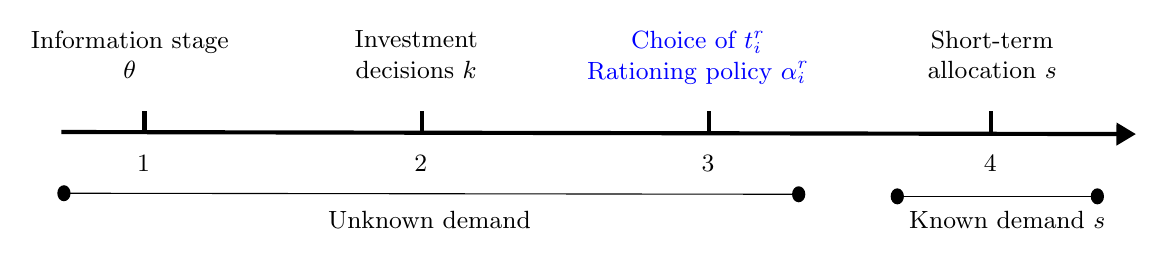
\begin{tikzpicture}[x=0.60pt,y=0.75pt,yscale=-1,xscale=1]

%Straight Lines [id:da9957648743256338] 
\draw [line width=1.5]    (20,100) -- (663,101) ;

\draw [shift={(667,101)}, rotate = 180.07] [fill={rgb, 255:red, 0; green, 0; blue, 0 }  ][line width=0.08]  [draw opacity=0] (11.61,-5.58) -- (0,0) -- (11.61,5.58) -- cycle    ;

%Straight Lines [id:da6515049842476789] 
\draw [line width=1.5,color = black]    (70,90) -- (70,100) ;
%Straight Lines [id:da5279432381947544] 
\draw [line width=1.5,color = black]   (237,90) -- (237,100) ;
%Straight Lines [id:da10457327739176892] 
\draw [line width=1.5,color = black]   (410,90) -- (410,100)  ;
%Straight Lines [id:da5055720939116881] 
\draw [line width=1.5,color = black]    (580,90) -- (580,100)   ;
%Straight Lines [id:da16737672008641513] 
\draw    (21.5,129.5) -- (464,130) ;
\draw [shift={(464,130)}, rotate = 0.06] [color={rgb, 255:red, 0; green, 0; blue, 0 }  ][fill={rgb, 255:red, 0; green, 0; blue, 0 }  ][line width=0.75]      (0, 0) circle [x radius= 3.35, y radius= 3.35]   ;
\draw [shift={(21.5,129.5)}, rotate = 0.06] [color={rgb, 255:red, 0; green, 0; blue, 0 }  ][fill={rgb, 255:red, 0; green, 0; blue, 0 }  ][line width=0.75]      (0, 0) circle [x radius= 3.35, y radius= 3.35]   ;
%Straight Lines [id:da35289334593742727] 
\draw    (523.39,131) -- (643.89,131) ;
\draw [shift={(643.89,131)}, rotate = 0] [color={rgb, 255:red, 0; green, 0; blue, 0 }  ][fill={rgb, 255:red, 0; green, 0; blue, 0 }  ][line width=0.75]      (0, 0) circle [x radius= 3.35, y radius= 3.35]   ;
\draw [shift={(523.39,131)}, rotate = 0] [color={rgb, 255:red, 0; green, 0; blue, 0 }  ][fill={rgb, 255:red, 0; green, 0; blue, 0 }  ][line width=0.75]      (0, 0) circle [x radius= 3.35, y radius= 3.35]   ;


% Text Node
\draw (0,50) node [anchor=north west][inner sep=0.75pt]  [font=\small] [align=center] {Information stage \\ $\theta$};
% Text Node
\draw (195,50) node [anchor=north west][inner sep=0.75pt]  [font=\small] [align=center] {Investment  \\ decisions $\displaystyle k$};
% Text Node
\draw (335,50) node [anchor=north west][inner sep=0.75pt]  [font=\small] [align=center] { \textcolor{blue}{Choice of $t^r_i$} \\ \textcolor{blue}{Rationing policy $\alpha_i^r$}};
% Text Node
\draw (540,50) node [anchor=north west][inner sep=0.75pt]  [font=\small] [align=center] {Short-term \\ allocation $\displaystyle s$};
% Text Node
\draw (179,137) node [anchor=north west][inner sep=0.75pt]  [font=\small] [align=center] {Unknown demand $ $};
% Text Node
\draw (529,137) node [anchor=north west][inner sep=0.75pt]  [font=\small] [align=center] {Known demand $\displaystyle s$ $ $};


\draw (64,110) node [anchor=north west][inner sep=0.75pt]  [font=\small] [align=left] {$1$};
% Text Node
\draw (231,110) node [anchor=north west][inner sep=0.75pt]  [font=\small] [align=left]  {$2$};
% Text Node
\draw (404,110) node [anchor=north west][inner sep=0.75pt]  [font=\small] [align=left]  {$3$};
% Text Node
\draw (574,110) node [anchor=north west][inner sep=0.75pt]  [font=\small] [align=center]  {$4$};

\end{tikzpicture}

\end{tcolorbox}

    %%%%%%%%%%%%%%%%%%%%    %%%%%%%%%%%%%%%%%%%%    %%%%%%%%%%%%%%%%%%%%    %%%%%%%%%%%%%%%%%%%%    %%%%%%%%%%%%%%%%%%%%    %%%%%%%%%%%%%%%%%%%%


% \subsection{Category-price policy}

We start by defining the rationing policy under this framework. This stage boils down to allocating the capacity $k_i$ in the first step between the two categories and the second step, randomly for each consumer within each category.

\begin{lemma}
The optimal share allocated to every group under the fixed-price allocation is the same as under the first-best allocation. The quantity of electricity allocated to category $i$ is then:

\begin{equation*}
    \alpha_i \; k = \int_{\Theta_i} q^*_i(\theta,s) dG_i(\theta)
\end{equation*}

And every consumer in the category $i$ receives: $\displaystyle \frac{\alpha_i k}{\mu_i}$.

\end{lemma}




We find that the market designer allocates the same expected quantity to each category under the first-best allocation even though the within-category allocation is inefficient. The problem is solved as follows. 

% Let the quantity for category $i$ be $q_i$; then, when the capacity is constraining, we must have for every state of the world: $\sum_{i} \mu_i q_i  = k$, implying that the relation between the quantity is equal to $q_i(q_j) = \frac{k - \mu_{j}q_j}{\mu_i}$. Then, we maximize the short-term expected utility given the previous relation. Solving using the first-order condition leads to a capacity share for each consumer belonging to a group $i$ equals the allocation under the first-best allocation. 


\subsection{Optimal single prices}


Given the rationing policy, we now describe the new problem the market designer faces. We define $s^r := s^r(\textbf{t}^r,k)$ as the first state of the world when the capacity is binding, given the set of fixed price $\textbf{t}^r = \{t^r_i\}_{i = \{1,2\}}$:

\begin{equation*}
\sum_{i} \mu_i \int_{\Theta_i} d(t^r_i,\theta,s^r) dG_i(\theta) = k
\end{equation*}

We note $S^r = [\ubar{s},s^r]$ as the set of off-peak periods during which the capacity is not biding and $T^r = (s^r,\overline{s}]$ as the set of on-peak periods during which the capacity is binding. Then, we define the expected aggregate consumer surplus in each set. This is key as prices do not affect consumers in the same way, depending on the period. The off-peak surplus is given by:

\begin{equation*}
    CS_S^r(k,\textbf{t}^r) = \sum_{i = \{1,2\} } \mu_i \int_{S^r} \int_{\Theta_i} \left( U(d(t^r_i,\theta,s),\theta,s) - t^r_i \; d(t^r_i,\theta,s) \right) dG_i(\theta) dF(\theta) 
\end{equation*}

and the on-peak surplus by:

\begin{equation*}
    CS_T^r(k,\textbf{t}^r) = \sum_{i = \{1,2\} } \mu_i \int_{T^r} \int_{\Theta_i} ( U\left(\frac{\alpha_i k}{\mu_i},\theta,s\right) - t^r_i \; \frac{\alpha_i k}{\mu_i} ) dG_i(\theta) dF(\theta)
\end{equation*}

When the capacity is not binding, the market allocation dictates how consumers choose their quantity given the set of prices $d(t^r_i,\theta,s)$. When the capacity is binding, then the market design has to really allocate the goods $\frac{\alpha_i k}{\mu_i}$. Two observations can be made at this stage. First, while the total quantity for each category is identical under the first-best and this framework, the total utility between the two environments does differ due to the concavity of the utility function. Second, due to the inefficient rationing and compared to the first-best case, the utility function is discontinuous in $s$ at the value $s = s^r$. Therefore, the marginal effect of the prices encompasses both the marginal change in the utility in both $S^r$ and $T^r$, but also how the delta of the utility at $s = s^r$. Similarly, the expected revenue from the mechanism is: 

\begin{equation*}
    R_S^r(k,\textbf{t}^r) = \sum_{i = \{1,2\} } \mu_i \int_{S^r} \int_{\Theta_i} t^r_i \; d(t^r_i,\theta,s)  dG_i(\theta) dF(\theta) 
\end{equation*}

and the on-peak surplus by:

\begin{equation*}
    R_T^r(k,\textbf{t}^r) = \sum_{i = \{1,2\} } \mu_i \int_{T^r} \int_{\Theta_i} t^r_i \; \frac{\alpha_i k}{\mu_i} dG_i(\theta) dF(\theta)
\end{equation*}


Then the optimal prices solves:

\begin{align*}
\max_{\substack{ \textbf{t}^r }}  \quad &  \quad   CS_S^r(k,\textbf{t}^r)  \quad  +  \quad CS_T^r(k,\textbf{t}^r) \quad  \\
  \text{s.t.} \quad &  \quad I(k)    \quad \leq   \quad   R_S^r(k,\textbf{t}^r) \quad  +  \quad R_T^r(k,\textbf{t}^r),         \tag{R}
\end{align*}




% We drop the capacity constraint as the rationing policy defines it implicitly. To see this, we can redefine the state of the world $s^r_1$ when the capacity starts binding: 

% \begin{equation*}
%    \sum_{i}\mu_i \int_{\Theta_i} d(t^r_i,\theta,s^r_1) dG_i(\theta) = k  
% \end{equation*}

It implies a very similar delta in terms of utility as the equation in the Appendix \ref{AppSec:singleprice} with a single price policy. We summarize the findings in the following proposition.

% First, let's note $\mathcal{L}^r$, the Lagrangian associated with the market designer program such that 

% \begin{equation*}
%     \mathcal{L}^r(k,t^r_1,t^r_2,\gamma^r) = CS^r(k,t^r_1,t^r_2) + \gamma^r R^r(k,t^r_1,t^r_2) 
% \end{equation*}

% With $CS^r$ the aggregate expected consumer surplus defined as the sum of consumers' utility net of monetary transfers, $\gamma^r$ the lagrangian multiplier associated with the revenue constraint, and $R^r(k)$ the revenue constraint (expected revenue net of investment costs). Then, using the Envelop Theorem, we can express the derivative of an optimal price with respect to $k_i$ as follows:

% \begin{equation}\label{eq:diffpri}
%     \pdv{t^r_i}{k} =  \big( {CS}_{ik} +  \rho_i CS_{jk} +  (R_i - \rho_i R_j) \gamma^r_k +  (R_{ik} - \rho_i R_{jk}) \gamma^r  \big) \frac{-\mathcal{L}_{jj}}{H^r}
% \end{equation}

% \begin{equation*}
%     \gamma^r_k =   -\frac{1}{bH^r}\left(\sum_{i} R_i ( L_{ij} L_{jk} - L_{jj} L_{ik} ) + R_k H^r \right)
% \end{equation*}

% pdv_lamb_v1 = ...
%     - (...
%     + pdv_net_R_inc_1_k * ( L11_l * L22_l - Lij_l^2 ) ...
%     + R1_l * ( - L22_l * L1k_l + Lij_l * L2k_l) ...
%     + R2_l * ( - L11_l * L2k_l + Lij_l * L1k_l) ...
%     )/(2 * R1_l * Lij_l * R2_l - L22_l * R1_l^2 - L11_l * R2_l^2) ;
% pdv_lamb_v1_fct = matlabFunction(pdv_lamb_v1);




% pdv_lamb_v2 = simplify(...
%    ( - pdv_net_R_inc_1_k * detHess_l ...
%     + R1_l * (  L22_l * CS1k_l - Lij_l * CS2k_l ) ...
%     + R2_l * (  L11_l * CS2k_l - Lij_l * CS1k_l ) ...
%     + R1_l * lamb_1 * ( L22_l * R1k_l - Lij_l * R2k_l ) ...
%     + R2_l * lamb_1 * ( L11_l * R2k_l - Lij_l * R1k_l ) ...
%     )/detBHess_l

% \begin{equation*}
%     \pdv{t^r_i}{k} =  \big( \overbrace{{CS}_{ik} +  \rho_i CS_{jk} }^{\text{consumer surplus effect} \leq 0} \quad + \quad \overbrace{  (R_i - \rho_i R_j) \gamma^r_k +  (R_{ik} - \rho_i R_{jk}) \gamma^r  }^{\text{revenue effect }\geq 0}  \quad \big) \underbrace{{\frac{-\mathcal{L}_{jj}}{H^r}}}_{\leq 0}
% \end{equation*}


% \begin{align}\label{eq:diffpri}
%     \pdv{t^r_i}{k} =&  \overbrace{\Bigg. \frac{-\mathcal{L}_{jj}}{H^r} \Bigg. }^{\leq 0} \overbrace{\Bigg( CS_{ik} +  \rho_i CS_{jk} +   (R_i - \rho_i R_j) \sum_{i}( CS_{ik} -\rho_i  CS_{jk} )\frac{ {  R_i } }{L_{jj} 
%  bH^r}}^{\text{effect of $k_i$ on CS with holding R fixed}}  \\ 
%    & \quad + \underbrace{  \gamma^r \bigg (R_{ik} - \rho_i R_{jk} + (R_i - \rho_i R_j)\sum_{i}(   R_{ik} - \rho_i R_{jk} ) \frac{ R_i  }{L_{jj} bH^r} \bigg)  -  R_k\frac{{ H^r} }{bH^r}   \Bigg) }_{\text{effect of $k_i$ on $R$}}
% \end{align}

% \begin{equation*}
%     \pdv{t^r_i}{k} =  \big( \Big. \overbrace{{CS}_{ik} + R_i \gamma^r_k + R_{ik}\gamma^r  \Big.  }^{\text{effect of $t^r_i$}} - \rho_i(\theta)  \overbrace{ \Big.{CS}_{jk}  + R_j  \gamma^r_k +  R_{ik} \gamma^r  \Big. }^{\text{effect of $p_j^r$}} ) \big) \underbrace{\Big.{\frac{-\mathcal{L}_{jj}}{H^r}}\Big.}_{\leq 0}
% \end{equation*}

% pdv_lamb_v1 = simplify(...
%     - (...
%     + pdv_net_R_inc_1_k * ( L11_l * L22_l - Lij_l^2 )..
%     + R1_l * ( - L22_l * L1k_l + Lij_l * L2k_l)..
%     + R2_l * ( - L11_l * L2k_l + Lij_l * L1k_l)..
%     )/detBHess_l);

% \begin{equation*}
%     \gamma^r_k =\frac{ \sum_{i}  R_i (L_{jj} L_{ik} - L_{ij} L_{jk}) - R_k H^r }{bH^r}
% \end{equation*}


% pdv_lamb_v2 = simplify(...
%    ( - pdv_net_R_inc_1_k * detHess_l...
%     + R1_l * (  L22_l * CS1k_l - CSij_l * CS2k_l - lamb_1 * Rij_l * CS2k_l )...
%     + R2_l * (  L11_l * CS2k_l - CSij_l * CS1k_l - lamb_1 * Rij_l * CS1k_l )...
%     + R1_l * lamb_1 * ( L22_l * R1k_l - Lij_l * R2k_l )...
%     + R2_l * lamb_1 * ( L11_l * R2k_l - Lij_l * R1k_l )...
%     )/detBHess_l);
% pdv_lamb_v2_fct = matlabFunction(pdv_lamb_v2);


% \begin{equation*}
%     \gamma^r_k =\frac{ \overbrace{\sum_{i}  R_i (  L_{jj} CS_{ik} - L_{ij} CS_{jk} )}^{\text{CS effect}} + \overbrace{\sum_{i} \gamma^r R_i (  L_{jj} R_{ik} - L_{ij} R_{jk} ) - R_k H^r}^{\text{Revenue effect}} }{bH^r}
% \end{equation*}


% With $\rho_i = \frac{L_{ij}}{L_{jj}}$. $H^r = \mathcal{L}_{11}\mathcal{L}_{22} - \mathcal{L}_{12}\mathcal{L}_{21}
% $ being the determinant of the Hessian matrix of the Lagrangian. $bH^r = \mathcal{L}_{ij} R_i R_j - \mathcal{L}_{jj} R_i^2 - \mathcal{L}_{ii} R_j^2 + \mathcal{L}_{ji} R_i R_j$ being the determinant of the bordered Hessian matrix of the lagrangian. Each variable's index is associated with the corresponding derivative. For instance, $CS_{ik}$ reads as the cross derivative between the price of category $i$ with respect to the investment level. It measures the (marginal) change of the marginal effect of price $ t^r_i$ on the consumer surplus. 


\begin{proposition}\label{propch3:prop4}
    Suppose that category 1 consumers are of higher types than category 2 consumers and that the investment cost is not too high then: (1) $t^r_1(k)$ is increasing with $k_i$; (2) $t^r_2(k)$ is first decreasing, then increasing with $k_i$.
\end{proposition}

\begin{proof}
In Appendix \ref{ch3app:Ap6}, we provide the formal proof and the condition under which the results hold. It relies on two Lemmas that ensure that a minimum exists. We also provide a more technical discussion on the rationales for this proposition. 
\end{proof}

Figure \ref{fig:optpolicypr1} illustrates the results. The red curve shows $t^r_1(k)$, the blue curve shows $t^r_2(k)$, and the black dashed curve shows the optimal single price $t^r(k)$ found in Appendix \ref{AppSec:singleprice}. Following the proposition, we observe that the blue curves corresponding to the group with a lower expected demand exhibit a non-monotonic relationship with the level of investment such that it decreases for low values of $k_i$ and then increases again following a similar behavior to the optimal price for the higher category of consumers represented in the red curve.


\begin{figure}
    \centering
    \includegraphics[scale = 1.2]{figure/optpolicypr1_pttv2.png}
    \caption{Optimal prices under the category-price policy with respect to the investment}
    \label{fig:optpolicypr1}
\end{figure}

The proof of such behavior of the optimal prices can be understood by distinguishing the first-order and the second-order effects of prices and level of investment on (a) the aggregate consumer surplus and (b) the revenue constraint. The non-monotonicities of prices are the result of a \textbf{consumer surplus effect} dominating first a \textbf{revenue effect} for low values of $k_i$, then the revenue effect dominating the consumer effect for higher values of $k_i$.


% We summarize this tension between consumer and revenue effects in the following equation, which is a more detailed expression of Equation \ref{eq:diffpri}.

% \begin{align*}
%     \pdv{t^r_i}{k} =&  \overbrace{\Bigg. \frac{-\mathcal{L}_{jj}}{H^r} \Bigg. }^{\leq 0} \Bigg( \overbrace{CS_{ik} +  \rho_i CS_{jk} +   (R_i - \rho_i R_j) \sum_{i}( CS_{ik} -\rho_i  CS_{jk} )\frac{ {  R_i } }{L_{jj} 
%  bH^r}}^{\text{effect of $k_i$ on CS with holding R fixed}}  \\ 
%    & \quad + \underbrace{  \gamma^r \bigg (R_{ik} - \rho_i R_{jk} + (R_i - \rho_i R_j)\sum_{i}(   R_{ik} - \rho_i R_{jk} ) \frac{ R_i  }{L_{jj} bH^r} \bigg)  -  R_k\frac{{ H^r} }{bH^r} }_{\text{effect of $k_i$ on $R$}}  \Bigg) 
% \end{align*}

As shown in Appendix \ref{AppSec:singleprice}, this framework implies that a change of $k_i$ does affect both revenue and the consumer surplus, which is captured via the direct effect on prices needed for financing this investment and the change of occurrences between off-peak and on-peak periods. First, the level of investment induces a positive first derivative of the consumer surplus and a negative second derivative. That is, increasing $k_i$ always increases the surplus, but for a higher level of investment, the positive impact is relatively smaller. On the other hand, an analysis of how the revenue constraint behaves shows a convex effect with respect to $k_i$. It implies that an increase of $k_i$ leads to the revenue constraint shifting at an increasing rate.\footnote{The pure revenue effect of increasing prices is found in Appendix \ref{AppSec:singleprice}. The intuition is that when $k_i$ increases, the marginal gain from an increase of capacity during on-peak periods is offset by the increase in investment costs and by the decrease of on-peak periods. In the Appendix, we formally demonstrate that $t^r$ is convex with respect to $k_i$.} The switch between the decreasing and increasing parts is associated with the consumer surplus effect dominating the revenue effect first. As $k_i$ increases, the respective concavity and convexity of the functions lead to the revenue effect dominating the surplus effect.

The increasing prices on the right part of Figure \ref{fig:optpolicypr1} can be understood through the results of Proposition \ref{propch3:prop3}. The ranking between the category prices stems from the preference for discriminating bigger consumers. Increasing $t^r_1$ generates more revenue as they consume, on average, more. 

Let us turn towards the left part of Figure \ref{fig:optpolicypr1}. We show why the asymmetry between the two consumers decreases for a higher value of $k_i$. Indeed, we find that this is not fully due to the revenue effect. For the sake of clarity, let's assume the revenue does not depend on $k_i$. We study the impact of $k_i$ on the indifference curve of the market planner with respect to the prices $t^r_1$ and $t^r_2$. We define the marginal rate of substitution between the two prices:


\begin{align*}
    MRS_{i \rightarrow j}(k) = \frac{CS^r_i}{CS^r_j}
\end{align*}

It implies that the MRS changes with respect to $k_i$ as follows:

\begin{align*}
    \pdv{MRS_{i \rightarrow j}}{k} = \frac{CS^r_{ik}CS^r_j - CS^r_{jk}CS^r_i}{{CS^r_j}^2}
\end{align*}

Therefore, the decreasing right part of prices can be explained by having $\pdv{MRS_{i \rightarrow j}}{k} < 0$. As the level of investment increases, and to keep the same level of consumer surplus, a decrease in $t^r_i$ should lead to a relatively smaller increase of $t^r_j$. The economic interpretation of the effect of $k_i$ can be understood as follows. As $k_i$ increases, it negatively impacts the (negative) marginal effect of prices on consumer surplus. Because consumers from the bigger category have a higher marginal consumer surplus with respect to price, the negative marginal effect of prices of $k_i$ is bigger than for the consumers from the smaller category. In other words, as $k_i$ increases, $CS_i$ decreases faster than $CS_j$, which implies a negative effect on the MRS. This can be explained by the fact that as $k_i$ increases, it lowers the occurrences of on-peak periods, which makes consumers more exposed to the negative price effect on the quantity during off-peak periods. This, in turn, incites the market designer to have lower prices, which is attained by lowering discrimination.

% We illustrate this intuition in Figure \ref{fig:illustTMS}. We represent a fixed revenue constraint as well as two indifference curves with respect to $t^r_1$ and $t^r_2$ for two values of $k_i$.  As $k_i$ increases, we show that the indifference curves tend to decrease in the sense that their marginal rate of substitution decreases with $k_i$. It is this shift in the shape of the consumer surplus that implies a decrease in the optimal price, meaning that the gain in lower prices is higher than the gain from discrimination.  

% \begin{figure}
%     \centering
%     \includegraphics{figure/illustTMS.png}
%     \caption{Illustration of the decreasing part of $t^r_2$ with respect to $k_i$}
%     \label{fig:illustTMS}
% \end{figure}



% We conclude this section by analyzing the implication of the optimal policy when choosing the level of investment to maximize the consumer surplus. We define the first-order conditions using the Envelop Theorem for constrained optimization. That is, it is sufficient to derive the derivative of the Lagrangian with respect to $k_i$: $\pdv{\mathcal{L}^r }{k} = \pdv{CS^r}{k} + \gamma^r \pdv{R^r}{k}$. We start with the individual consumer surplus\footnote{We use the individual surplus for clarity. The aggregate surplus exhibits similar behavior.}:

% \begin{align*}
%          &  \overbrace{   \int_{\alpha_i^r k}^{d(t^r_i,\theta,s^r_1)} u(q,\theta,s^r_1) dq }^{\text{$\Delta$ in quantity btw. off-peak and on-peak}}+ \overbrace{\int_{s^r_1}^{\overline{s}} ( u( \alpha_i^r k, \theta,s) - t^r_i) dF(s)}^{\text{$+$ in on-peak CS}} 
% \end{align*}

% The second term is similar to the complete information benchmark. It represents the gain in consumer surplus during on-peak as capacity expands. Note that the gain in surplus does not depend on the price as the quantity is randomly assigned to each consumer in each category due to imperfect information. The first term stands for the change at the margin of quantities for each consumer. Under complete information, the quantities allocation is continuous in $s$. However, due to incomplete knowledge, the market designer creates a discontinuity in the allocation when capacity starts binding, which implies that the value at $s^r_1$ does not cancel out. For the revenue, the derivative can be expressed as follows: 

% \begin{align*}
%          &  \overbrace{ \Bigg. \sum_{i}\mu_i \int_{\Theta_i} t^r_i \bigg( d(t^r_i,\theta,s^r_1) - \alpha_i^r k \bigg) dG_i(\theta)  \Bigg.}^{\text{$\Delta$ in quantity btw. off-peak and on-peak}}+ \overbrace{\int_{s^r_1}^{\overline{s}}  \Bigg. \sum_{i}\mu_i t^r_i dF(s)\Bigg. }^{\text{$+$ in on-peak rev.}}   - r
% \end{align*}

% The first term is similar and originates from discontinuity. The second term comes from the increase in available quantity during on-peak. As expected, and similarly to the first-best investment level, the sign of the first-order condition is ambiguous as it has positive and negative effects of an increase in $k_i$. For instance, it raises investment costs, but it also raises available revenue. Calculations show that a level of investment exists that maximizes the expected aggregate consumer surplus, as the consumer surplus and the revenue are concave in $k_i$. 






\section{Conclusion}\label{chap3sec:sec6}

This paper built a theoretical framework to analyze the role of market designers in finding the most efficient way of consuming an essential good when faced with investment decisions. Most of the literature has focused either on providing additional remuneration streams for producers to increase the level of investment or on designing the second-best pricing schedule for consumers, given informational and technical constraints. This paper provides a unifying framework linking investment decisions and consumer participation. We show an inherent tension when implementing an allocation mechanism to maximize consumer surplus and generate revenue to cover fixed costs. The paper provides policy and technical results by adding additional constraints to the initial framework. We assume that consumers possess private information with respect to their utility level and that the market designer may be constrained in the allocation mechanism he can propose to consumers. The central result of the paper is that, depending on a set of assumptions, some specific and non-intuitive relations exist between the level of investment and the optimal allocation proposed to consumers, which has significant welfare and distributive implications. We first introduce incomplete information in a contemporaneous setting. That is, we model a market designer who cannot set prices for every state of the world. This framework shows that the market designer faces a trade-off between generating a higher surplus by discriminating against smaller consumers and generating higher revenue to finance investment by discriminating against bigger consumers. In the end, smaller consumers from the smaller category favor a high level of investment, and bigger consumers from the bigger category favor a low investment level. In the last section, we adopt a standard mechanism design approach to consider incentive and participation constraints. The central highlight is the specific relation between the level of investment and the individual and aggregate information rent. We find that only bigger consumers can face an increase both in quantity and surplus when the level of investment is high as they are the only consumers to face an increasing information rent with respect to the capacity level.

Finally, we plan to extend the result with two main extensions: (i) study market design constraints with the mechanism design framework. While market designers may wish to implement some information revelation mechanism, as theoretically studied in the third result, practical contractual arrangements between the market designer and consumers may constrain him in the implementable mechanism. It would lead to specific effects, as highlighted in the second set of results. (ii) Implement specific distribution preferences associated with consumer types and categories. The current framework does not consider welfare weights, which may distort the optimal allocation. Including such parameters would highlight the tension between generating sufficient revenue and maximizing consumer surplus. From a more extreme view, as the paper shows, the allocation can exhibit some non-monotonicities of the optimal quantities and prices; a market designer may want to avoid any decreasing quantities when the level of investment rises. Including such constraints in the framework could highlight new trade-offs.




\appendix



\section{Single price policy}\label{AppSec:singleprice}

We start by assuming that the market designer is constrained by setting a unique price for each category, so we drop the index and assume that $t^r$ is the price chosen by the market designer. The incomplete information set-up in this section has an important implication regarding quantity allocation. Indeed, combining a single-price policy and imperfect knowledge implies that some inefficient rationing should be expected in the market. To see this, recall that $d(t^r,\theta,s)$ is the quantity a consumer asks given the price $t^r$. Let's define $s^r_0$ the first states of the world when the capacity is binding when the price is $t^r$, that is:

\begin{equation*}
 \sum_{i}\mu_i \int_{\Theta_i} d(t^r,\theta,  s^r_0 ) dG_i(\theta) = k    
\end{equation*}

We note $S^r_0 = [\ubar{s},s^r_0]$ as the set of off-peak periods during which the capacity is not biding and $T^r_0 = (s^r_0,\overline{s}]$ as the set of on-peak periods during which the capacity is binding. For any $ s \in S^r_0$, the price is such that capacity is not binding. That is, the quantity asked by each consumer is short-term. In that case, there is no need for rationing. Note, however, that when $t^r > 0$, the model does imply an inefficiency similar to the effect of market power. Due to the price being higher to marginal, it prevents some Pareto-improving trade from happening. For any $s \in T^r_0$, capacity is binding, and the total quantity each consumer asked is above the available capacity. To avoid market failure, the market designer needs to reallocate quantity between consumers. However, we assumed that he does not observe consumer type. Without any possibility of extracting information, the only option for the market designer is to allocate a quantity equal to the investment level equally across consumers. Therefore, the individual quantity $k_i$ and the expected quantity for each category is $\mu_i k$. We illustrate the implications by defining the expected utility under the single-price policy with incomplete information.

\begin{equation*}
     \sum_{i}\mu_i \quad \overbrace{\int_{S^r_0} \int_{\Theta_i} U(d(t^r,\theta,s),\theta,s) dG_i(\theta) dF(s)}^{\text{off-peak utility}} +  \overbrace{\int_{T^r_0}\int_{\Theta_i} U(k ,\theta,s) dG_i(\theta) dF(s)}^{\text{on-peak utility}}
\end{equation*}

We now determine the best single-price policy given the framework. Compared to the previous analysis, the optimal price $t^r$ depends not only on the first-best condition but on the revenue constraint. If it exists, the optimal value $t^r$ satisfies the net revenue condition $R^r_0(k,t^r) = 0 $ with:

\begin{equation*}
    R^r_0(k,t^r):= t^r  \quad \underbrace{\left(\sum_{i}\mu_i \int_{S^r_0} \int_{\Theta_i} d(t^r,\theta,s) dG_i(\theta) dF(s) + \int_{T^r_0}  k dF(s) \right)}_{\text{Expected quantity}} \quad -  \quad  I(k) 
\end{equation*}
    
This observation is close to what can be found in the literature on peak pricing with price-inelastic consumers. In that case, the optimal price is simply the average cost. Under the framework, the optimal single price is different due to the price response of the consumers during off-peak periods and to the inefficient rationing occurring in the on-peak periods.  Next, we provide in Proposition \ref{propch3:prop3} the relation between the investment level and the optimal single-price

\begin{proposition}\label{propch3:prop3}
        If an optimal single-price $t^r(k)$ exists, it increases in $k_i$.
\end{proposition}
\begin{proof}
See Appendix \ref{ch3app:Ap5}
\end{proof}

Proposition \ref{propch3:prop3} shows that expanding the capacity level always leads to the positive (revenue) effect dominating the adverse (price) effects. That is, the effect of the increase in the revenue collected during on-peak periods offsets the compound negative impact of a price increase that (may) lower the revenue during off-peak periods and reduces the occurrence of on-peak periods. In other words, the market designer never lowers the price so as to increase consumption during off-peak.

When choosing the price $t^r$, the market designer must trade off opposite effects. Indeed, increasing $t^r$ lowers quantity during off-peak. Hence, the revenue effect during off-peak is ambiguous. For on-peak periods, the revenue effect is always positive as the expected quantity is $k_i$ and is not affected by a change of $t^r$. Note that the revenue is concave in $t^r$, meaning that the second-order effects are negative, limiting the market designer's ability to extract revenue from consumers.\footnote{Increasing $t^r$ lowers the occurrence of on-peak periods, and the revenue during off-peak is concave due to the linearity assumption of the marginal utility.} Those effects can be shown by expressing the first  derivative of the expected net revenue:
    
\begin{align*}
    \pdv{R^r}{t^r} =\underbrace{  \int_{S^r} \big( \overbrace{\bigg. d_t t^r \bigg.}^{\text{price effect }-}   + \overbrace{\bigg.\sum_{i} \mu_i \int_{\Theta_i}   d(t^r,\theta,s) \bigg.  dG_i(\theta)  }^{\text{quantity effect }+} \big)dF(s)}_{\text{off-peak marg. revenue}} + \underbrace{\overbrace{\int_{T^r} \bigg. 
k \bigg. dF(s) }^{\text{quantity effect }+}}_{\text{on-peak marg. revenue}}
\end{align*}

With $d_t = \pdv{d}{t}$ the derivative of the demand function with respect to prices. Intuitively, the set $S_0^r$ is increasing in $t^r$ as we have $\pdv{s_0^r}{t^r} > 0 $. A higher price implies that consumers decrease their consumption, and the capacity is binding less often. The proof relies on the observation that the second derivative is always negative. Hence, the revenue is concave in $t^r$. Next, we show how $k_i$ modifies the expected revenue. An increase in the investment level leads to more investment costs and an increase in the quantity during on-peak periods. In other terms, the gain in on-peak periods cannot compensate for the loss due to the investment costs. Then, we use the fact that $R^r(k)$ is concave in $t^r$, and we study its behavior at the limit case such that the value $k_i$ implies that the capacity always binds (i.e., $s_0^r(k) = 0$). In that case, we have $t^r = r$. Moreover, we also have at this limit: $\pdv{R}{{t^r}} > 0 $, implying that the revenue is increasing at the limit in $t^r$. If the function is concave, there could be at most two potential values for the optimal value of $t^r$. However, the consumer surplus is always decreasing in prices; therefore, a lower price is always optimal compared to a higher price. So, the optimal value corresponds to the first increasing part. As $ R^r(k)$ is always decreasing in $k_i$, the solution of $R^r(k)$ is also increasing with $k_i$.


\section{Two-parts tariff}

When $k \in K^-$ 


Let's define $\theta^r := \theta^r(p,A)$ such 

\begin{equation*}
    \int_{\mathcal S} (U(d(t^r,\theta^r,s) - A - t^r d(t^r,\theta^r,s) ) dF(s) = 0  
\end{equation*}

Note that the threshold is the same for the two categories of consumers. The set of consumers participating in the market from the category $i$ is given by $\boldsymbol{\uptheta}_i = (\theta_i^r , \overline{\theta}_i)$. The expected aggregate quantity is then: 

\begin{equation*}
    \E{Q_{\boldsymbol{\uptheta}}}(t^r) = \sum_{i = \{1,2\} } \mu_i \int_{\mathcal S}  \int_{\boldsymbol{\uptheta}_i}  d(t^r,\theta,s) dG_i(\theta) dF(s)
\end{equation*}

The average quantity:

\begin{equation*}
    \E\tilde{Q_{\boldsymbol{\uptheta}}}(t^r) = \frac{ \E{Q}(t^r)}{\sum_{i = \{1,2\} } \mu_i \int_{\mathcal S}  \int_{\boldsymbol{\uptheta}_i}g_i(\theta) d\theta}
\end{equation*}

The expected quantity demanded by the indifferent consumer in both groups:

\begin{equation*}
    \E d(t^r,\theta^r) =  \int_{\mathcal S}  d(t^r,\theta^r,s)  dF(s)
\end{equation*}

And the expected derivative:

\begin{equation*}
    \E Q_{\boldsymbol{\uptheta}}'(t^r) = \sum_{i = \{1,2\} } \mu_i \int_{\mathcal S}  \int_{\Theta_i}  d'(t^r,\theta,s) dG_i(\theta) dF(s)
\end{equation*}


We denote the price elasticity of demand is $\varepsilon_p = \E Q_{\boldsymbol{\uptheta}}'(t^r) \frac{t^r}{\E Q_{\boldsymbol{\uptheta}}(t^r)}$. Then, the optimal two-part tariff satisfies the following condition.

\begin{equation*}
    1 = \frac{1}{1 + \varepsilon} \frac{1}{\varepsilon_p} \left[ 1 - \frac{\E d(t^r,\theta^r)}{\E\tilde{Q_{\boldsymbol{\uptheta}}}(t^r)}  \right]
\end{equation*}

With only a single price, the optimal $t^r$ is the average cost given by:

\begin{equation*}
    t^r = \frac{I(k)}{ \E{Q}(t^r)}
\end{equation*}

With 
\begin{equation*}
    \E{Q}(t^r) = \sum_{i = \{1,2\} } \mu_i \int_{\mathcal S}  \int_{\Theta_i}  d(t^r,\theta,s) dG_i(\theta) dF(s)
\end{equation*}

When $k \in k^+_i$ 


\section{Individual welfare effect}\label{AppSec:indivwelfare}

We now compare the outcomes in terms of welfare given the optimal policy for the single-price and category-based prices. We focus the analysis on the individual change in the consumer surplus from a switch from a single-price-based policy to a category-based one.\footnote{Note that the individual welfare changes with respect to $k_i$ for each consumer are not relevant in this section as prices are based on category. Therefore, each consumer in its corresponding category exhibits similar surplus behavior. 
 This motivates the study of this section of the evolution of the change of welfare from the two policies with respect to $k_i$.} In this section and for clarity, we focus on the consumer surplus change for a given $k_i$ and rather on the change based on difference maximizing investment level that might differ from the two policies.

We start by noting that the occurrence of on-peak situations can be higher for both policies depending on the values of prices: under the framework, this boils down to comparing the average category prices (weighted by the share of consumers) to the single price $s_1^r(t^r_1,t^r_2) - s_0^r(t^r) = \sum_{i}\mu_i  t^r_i -  t^r $. For instance, if $  t^r - \sum_{i}\mu_i  t^r_i < 0 $, then the prices under the category-based policy are relatively higher than under the single-price policy, implying that consumers reduce their consumption during off-peak under the former policy, and capacity binds more often. In any case, the change of individual surplus can be decomposed into three terms composed of two terms. We illustrate the change in the following equation for a consumer of type $\theta$ and belonging to category $i$ (with $t^r > \sum_{i}\mu_i  t^r_i $). 

\begin{align*}
     \Delta_i CS(\theta) =  &  \int_{0}^{s_1^r(t^r_1,t^r_2)} (\Delta_i U1 + \Delta_i R1)  dF(s) + \int_{s_1^r(t^r_1,t^r_2)}^{s_0^r(t^r)} (\Delta_i U2 + \Delta_i R2)   dF(s)   \\ & + \int_{s_0^r(t^r)}^{\overline{s}}( \Delta_i U3 + \Delta_i R3)   dF(s) 
\end{align*}

$\Delta U$ captures the change in utility due to the price effect during off-peak periods on the quantity and the rationing policy under on-peak periods. For instance for a consumer belonging to category $i$: we have: $\Delta U_1 = U(d(t^r_i,\theta,s),\theta,s) - U(d(t^r,\theta,s),\theta,s)$. $\Delta R$ represents the change in the payment from each consumer. That is, for a consumer belonging to category $i$ we have $\Delta R_1 = t^r d(t^r,\theta,s) - t^r_i d(t^r_i,\theta,s) $. Hence, the individual effect from discrimination is captured following the expected change in each term. 

The framework prevents us from having any closed-form solution. Therefore, we concentrate the analysis on the main drivers of the welfare effect. Indeed, simulation shows that the second term in the previous equation is relatively small compared to the first and third terms. In other words, while there is a difference in terms of the occurrence of on-peak periods between the two policies, the delta between $s_1^r(t^r_1,t^r_2)$ and $s_0^r(t^r) $ is relatively small compared to other orders of magnitude. Hence, we discard it from the analysis. We summarize the analysis of the individual change in the following claim. Without loss of generality, we assume that category $1$ is of a higher type than category 2.

% We then distinguish two types of change: the ones that depend on the consumer type $\theta$ and the ones that are independent. 


% In this environment, $\Delta_i U1$ and $\Delta_i R3$ are independent of $\theta$ for every consumer. This is due to the linear marginal utility for $\Delta_i U1$ and to the fact that the quantity during on-peak periods is allocated randomly in both policies for $\Delta_i R3$. In the case of $\Delta_i U1$, the sign of its value is solely dependent on $\Delta_i t^r =  t^r - t^r_i $, as we have $\Delta_i U1 = \frac{1}{2}({t^r}^2 - {t^r_i}^2)$. In the case of $\Delta_i R3$, the sign is given by $k\Delta_i t^r  - \mu_{-i} t^r_i \Delta_i \theta^{av}$, with $\Delta_i \theta^{av}$ the difference between the average values : $\Delta_i \theta^{av} = \theta_i^{av} - \theta_{-i}^{av}$.\footnote{Note that if we assume that a category $i$ has bigger consumers then $\theta_i^{av}>\theta_{-i}^{av}$.} On the other hand, $\Delta_i R1$ and $\Delta_i U3$ are dependent on $\theta$, but they can also be decomposed between a dependent and an independent part. In the case of $\Delta_i R1$, we rewrite the term such that $\Delta_i R1 = \Delta_i R1^{\theta} + \Delta_i R1^c$ with  $\Delta_i R1^{\theta} = \theta \Delta_i t^r$ and $\Delta_i R1^c  = (s - \Delta_i t^r)\Delta_i t^r$, the first term depends on $\theta$ while the second does not. In the case of $\Delta_i U3$, we rewrite the term such that $\Delta_i U3  = \Delta_i U3^{\theta} + \Delta_i U3^c$ with $ \Delta_i U3^{\theta} = \mu_{-i}\Delta_i \theta^{av}\theta $ and $ \Delta_i U3^c = \mu_{-i}\Delta_i \theta^{av}\left( s  - k - 0.5 \mu_{-i} \Delta_i \theta^{av} \right)$.  

\begin{claim}

When the category-based policy is implemented, individual consumer surplus for consumers of category 1 (resp. category 2) increases (resp. decreases) with low values of $k_i$. It decreases (resp. increases) with high values of $k_i$. Moreover, individual consumer surplus for smaller consumers from category 1 (resp. category 2) sustains smaller (resp. greater) gains and greater (resp. smaller) losses from the change in policy.

\end{claim}

The results in the Claim can be understood as a mirror effect from one category to another both in terms of magnitude and of who gets more impacted by the change of policy. The results are illustrated in Figure \ref{fig:relativechangepr}. The within-category comparison is clearly stated in $\Delta_i R1^{\theta} = \theta \Delta_i t^r$ and $ \Delta_i U3^{\theta} = \mu_{-i}\Delta_i \theta^{av}\theta $. Whatever the sign of those terms, the smaller the $\theta$, the smaller the change. Then, we find that the main gains for the larger category come from $\Delta_i U3$, while it is the main source of losses for the smaller category. Switching from a single-price-based policy to a category-based policy increases the utility of the consumers from category 1 as they are allocated a greater share of quantity when the capacity is binding. However, as $k_i$ increases, the capacity binds less in terms of occurrences. It implies that the main utility gain for the higher category (and the main loss for the smaller category) decreases as $k_i$ increases. For $\Delta_i U1$ and $\Delta_i R1$, the sign (mostly) depends on $\Delta_it^r$. When $k_i$ increases, we previously showed that there is a switch in terms of ranking between $t^r_1$ and $t^r_2$, namely that for high values of $k_i$ we have: $t^r_1 > t^r > t^r_2 $. In that case we have $\Delta_1 U1 < 0$ and $\Delta_2 U1 > 0$. For $\Delta_i R3 = k\Delta_i t^r  - \mu_{-i} t^r_i \Delta_i \theta^{av}$, the sign is ambiguous. However, for higher values of $k_i$, the change for the higher category is negative as we have $\Delta_1 t^r < 0 $ and $\Delta_1 \theta^{av} > 0$. In other terms, the main losses for the higher type come from the difference in prices and are also mostly localized during off-periods. As $k_i$ increases, the price differential increases, and it also increases the occurrences of off-peak periods. All in all, a higher level of investment means more losses for the higher category and more gains for the lower category. Finally, as the common net effect ($\Delta_i U1, \Delta_iR3 $ ) is negative for the higher category and positive for the lower category, the smaller consumers are more negatively affected for the higher category and positively affected for the smaller category. 


\begin{figure}
    \centering
    \includegraphics{figure/relativechangepr.png}
    \caption{Change in consumer surplus with respect to investment level and consumer type. Consumers from the higher category exhibit a high gain from the switch to a category-based policy with a low level of investment. On the other hand, consumers from the lower favor a higher level of investment. Moreover, smaller consumers from the higher category sustain lower gains, which is the opposite for smaller consumers from the lower category.}
    \label{fig:relativechangepr}
\end{figure}


\section{Proof of Proposition \ref{lemm1}} \label{ch3app:Ap1}

XXXX


\section{Proof of Proposition \ref{propch3:prop4}}\label{ch3app:Ap6}
\begin{proof}
We denote the consumer surplus under the policy as follows:

\begin{align}\label{eq:CSri}
     CS^r(k,t^r_i,t_j^r)  = & \sum_{i} \mu_i \left[\int_0^{s_1^r(k)}  \int_{\Theta_i} \left( U(d(t^r_i,\theta,s),\theta,s) -  t^r_i d(t^r_i,\theta,s) \right)dG_i(\theta) dF(s) \right. \\
     \nonumber + & \left.\sum_{i} \mu_i \int_{s_1^r(k)}^{\overline{s}}  \int_{\Theta_i} \left( U(\alpha_i^r(k) k ,\theta,s) -  t^r_i \alpha_i^r(k) k \right)dG_i(\theta) dF(s)   \right]
\end{align}

With $\alpha_i^r(k) = 1 + \frac{  \mu_j (\theta^{av}_i - \theta^{av}_j )}{k}$ corresponding to the share of capacity allocated to category $i$. $s_1^r(k)$ is given by solving: $\sum \mu_i \int_{\Theta_i} d(t^r_i,\theta,s_1^r(k)) dG_i(\theta) = k $. Which gives :

\begin{equation}\label{eq:s1pr1}
      s_1^r(k) = k + \sum_{i} \mu_i (t_i^r - \theta_i^{av}) 
\end{equation}

The expected revenue net of investment costs is defined as:

\begin{align}\label{eq:Rri}
    R^r(k,t_i^r,t_j^r)  = & \sum_{i} \mu_i \left[\int_0^{s_1^r(k)}  \int_{\Theta_i} \left(  t^r_i d(t^r_i,\theta,s) \right)dG_i(\theta) dF(s) \right. \\
     + & \left.\sum_{i} \mu_i \int_{s_1^r(k)}^{\overline{s}}  \int_{\Theta_i} \left( t^r_i \alpha_i^r(k) k \right)dG_i(\theta) dF(s)   \right] - I(k)
\end{align}

Hence, the maximization problem is given in the following expression:

\begin{align*}
\max_{\substack{ k,\\ t^r_i \rightarrow \mathbb{R}^+}}  \quad \quad &  CS^r(k,t_i^r,t_j^r) \quad  \\
  \text{s.t.} \quad\quad & 0 \leq  R^r(k,t_i^r,t_j^r) ,         \tag{R}
\end{align*}

The Lagrangian associated with the market designer program such that 

\begin{equation*}
    \mathcal{L}^r(k,t_i^r,t_j^r) = CS^r(k,t_i^r,t_j^r) + \gamma R^r(k,t_i^r,t_j^r) 
\end{equation*}

With $\gamma^r$, the lagrangian multiplier is associated with the revenue constraint. The first-order condition of the program at the optimal value of $t_i^r(k)$ and $t_j^r(k)$ are equal to:

\begin{align*}
    \begin{cases}
    CS^r_i(k,t_i^r,t_j^r) + \gamma(k) R^r_i(k,t_i^r,t_j^r) = 0 \\
    CS^r_j(k,t_i^r,t_j^r) + \gamma(k) R^r_j(k,t_i^r,t_j^r) = 0
    \end{cases}
\end{align*}

With $CS^r_i(k,t_i^r,t_j^r) = \pdv{CS^r(k,t_i^r,t_j^r)}{t^r_i}$ and $R^r_i(k,t_i^r,t_j^r)  = \pdv{R^r(k,t_i^r,t_j^r)}{t^r_i}$. Differentiating with respect to $k_i$ the first equation and dropping the variables for clarity implies that: 

\begin{align*}
      CS^r_{ii}\pdv{t^r_i(k)}{k} + \gamma(k) R^r_{ii}\pdv{t^r_i(k)}{k} + CS^r_{ij}\pdv{t^r_j(k)}{k} + \gamma(k) R^r_{ij}\pdv{t^r_j(k)}{k} + CS^r_{ik} + \gamma(k) R^r_{ik} + \pdv{\gamma(k)}{k}R^r_{i}  = 0
\end{align*}

With $ CS^r_{ii} = \pdv[2]{CS^r}{{t_i^r}}$, $ R^r_{ii} = \pdv[2]{R^r}{{t_i^r}}$, $ CS^r_{ij} = \frac{\partial CS}{\partial t_i^r \partial t_j^r}$ , $ R^r_{ij} = \frac{\partial R}{\partial t_i^r \partial t_j^r}$  , $ CS^r_{ik} = \frac{\partial CS}{\partial t_i^r \partial k}$ , $ R^r_{ik} = \frac{\partial R}{\partial t_i^r \partial k}$. The equation simplifies to:

\begin{align*}
      \mathcal{L}_{ii}^r(k,t_i^r,t_j^r)\pdv{t^r_i(k)}{k} + \mathcal{L}_{ij}^r(k,t_i^r,t_j^r)\pdv{t^r_j(k)}{k} + \mathcal{L}_{ik}^r(k,t_i^r,t_j^r) + \pdv{\gamma(k)}{k}R^r_{i}(k,t_i^r,t_j^r)  = 0
\end{align*}

With $ \mathcal{L}_{ii}^r$,$ \mathcal{L}_{ij}^r$ and $ \mathcal{L}_{ik}^r$ the derivatives of the Lagrangian. Hence, the derivatives of the first-order condition are given by:

\begin{align*}
    \begin{cases}
      \mathcal{L}_{ii}^r(k,t_i^r,t_j^r)\pdv{t^r_i(k)}{k} + \mathcal{L}_{ij}^r(k,t_i^r,t_j^r)\pdv{t^r_j(k)}{k} + \mathcal{L}_{ik}^r(k,t_i^r,t_j^r) + \pdv{\gamma(k)}{k}R^r_{i}(k,t_i^r,t_j^r)  = 0 \\\\
     \mathcal{L}_{jj}^r(k,t_i^r,t_j^r)\pdv{t^r_j(k)}{k} + \mathcal{L}_{ji}^r(k,t_i^r,t_j^r)\pdv{t^r_i(k)}{k} + \mathcal{L}_{jk}^r(k,t_i^r,t_j^r) + \pdv{\gamma(k)}{k}R^r_{j}(k,t_i^r,t_j^r)  = 0
    \end{cases}
\end{align*}

Which implies : 

\begin{align*}
    \begin{cases}
      \pdv{t^r_i(k)}{k} =  - \left( \mathcal{L}_{ij}^r(k,t_i^r,t_j^r)\pdv{t^r_j(k)}{k} + \mathcal{L}_{ik}^r(k,t_i^r,t_j^r) + \pdv{\gamma(k)}{k}R^r_{i}(k,t_i^r,t_j^r)  \right) \frac{1}{\mathcal{L}_{ii}^r(k,t_i^r,t_j^r)}  \\\\
    \pdv{t^r_j(k)}{k} =  - \left( \mathcal{L}_{ji}^r(k,t_i^r,t_j^r)\pdv{t^r_i(k)}{k} + \mathcal{L}_{jk}^r(k,t_i^r,t_j^r) + \pdv{\gamma(k)}{k}R^r_{j}(k,t_i^r,t_j^r)  \right) \frac{1}{\mathcal{L}_{jj}^r(k,t_i^r,t_j^r)}
    \end{cases}
\end{align*}

Let's note the determinant of the Hessian matrix of the Lagrangian $H^r = \mathcal{L}_{ii}^r\mathcal{L}_{jj}^r  - \mathcal{L}_{ij}^r\mathcal{L}_{ji}^r$. Then the derivative of the optimal value of $t^r_i(k)$ with respect to $k_i$ is equal to:


\begin{equation}
    \pdv{t^r_i(k)}{k} =  \left( \mathcal{L}_{ik}^r(k,t_i^r,t_j^r) + R_i  \pdv{\gamma(k)}{k} -  \rho_i \left( \mathcal{L}_{jk}^r(k,t_i^r,t_j^r) + R_j \pdv{\gamma(k)}{k} \right) \right) \frac{-\mathcal{L}_{jj}}{H^r}
\end{equation}

With $\rho_i = \frac{L_{ij}}{L_{jj}}$. The revenue constraint gives the expression of the derivative of the Lagrangian multiplier. As it is binding, we have the revenue at the optimal values:

\begin{align*}
  R^r(k,t_i^r(k),t_j^r(k)) = 0 
\end{align*}

Hence:

\begin{align*}
  R^r_i(k,t_i^r(k),t_j^r(k)) \pdv{t^r_i}{k} + R^r_j(k,t_i^r(k),t_j^r(k)) \pdv{t^r_j}{k} + R^r_k(k,t_i^r(k),t_j^r(k)) = 0 
\end{align*}

From the previous findings on the derivative of the optimal values $t^r_i(k)$ and $t^r_j(k)$, we have:

\begin{align*}
  R^r_i(k,t_i^r(k),t_j^r(k)) \left( \mathcal{L}_{ik}^r(k,t_i^r,t_j^r) -  \rho_i \mathcal{L}_{ij}^r(k,t_i^r,t_j^r) +  (R_i - \rho_i R_j) \pdv{\gamma(k)}{k} \right) \frac{-\mathcal{L}_{jj}}{H^r} \\
  + R^r_j(k,t_i^r(k),t_j^r(k)) \left( \mathcal{L}_{jk}^r(k,t_i^r,t_j^r) -  \rho_j \mathcal{L}_{ji}^r(k,t_i^r,t_j^r) +  (R_j - \rho_i R_i) \pdv{\gamma(k)}{k} \right) \frac{-\mathcal{L}_{ii}}{H^r} \\
  + R^r_k(k,t_i^r(k),t_j^r(k)) = 0 
\end{align*}

It implies that: 

\begin{equation*}
    \pdv{\gamma(k)}{k}  =   -\frac{1}{bH^r}\left(\sum_{i} R_i  ( \mathcal{L}_{ij}^r  \mathcal{L}_{jk}^r  - \mathcal{L}_{jj}^r  \mathcal{L}_{ik}^r  ) + R_k H^r \right)
\end{equation*}


In the next step, we formally prove that at least one minimum exists for the price of the smaller category. The critical insight of the proof relies on the behavior of prices in the special cases of the maximization program. That is when the capacity level is such that it always binds or it never binds in expectation. The following results show that the prices are always increasing with a relatively high level of $k_i$ when the capacity never binds, and the price of the smaller consumer at the level of investment such that it always binds is always decreasing. For the price of the bigger consumer, the result is ambiguous as it may happen that for some values of the parameters, the price might decrease. We also provide a more detailed discussion of the rationale behind such behavior in the proof.


\begin{lemma}\label{lem:AppLem1}

Assume that for a given $k_i$, the optimal values $t_i^r(k)$ and $t_j^r(k)$ are such that $s_1^r(k) > \overline{s}$. Then $t_i^r(k)$ and $t_j^r(k)$ are increasing and convex in $k_i$. Moreover, if $i$ is the bigger category then we have $t_j^r(k) > t_i^r(k)$.

\end{lemma}

\begin{proof}

Assuming that the capacity never binds in expected significantly implies the analysis. All the cross derivatives are null, and the second derivatives for both the consumer surplus and the revenue with respect to $k_i$ are also null. The derivative of the optimal price $t_i^r(k)$ is equal to:

\begin{equation*}
    \pdv{t_i^r(k)}{k} = -\pdv{\gamma(k)}{k}\frac{R_i}{\mathcal{L}_{ii}}
\end{equation*}

With $R_i>0$. Indeed, the revenue is concave in $t_i^r$ : $R_{ii} = - 2 \mu_i \int_{\mathcal S} 1 dF(s) <0 $. Hence, there are at most two possible values that can satisfy the revenue constraint. As the market designer always prefers smaller prices for consumers, then the chosen value is the minimum of the two, which, under a concave function, is located in the increasing part of the function. Next, we have $\mathcal{L}_{ii} = \mu_i(1 - 2\gamma(k))$. We prove that $\gamma(k)>1$, hence $\mathcal{L}_{ii} < 0$. From the maximization problem, we have : 

\begin{equation*}
    \gamma(k) = - \frac{CS^r_i}{R_i}
\end{equation*}

With 

\begin{equation*}
    CS^r_i = - \mu_i \int_{\mathcal S}  \int_{\Theta_i}  d(t_i^r,\theta,s) dG_i(\theta) dF(s) 
\end{equation*}

And 

\begin{equation}\label{eq:pdvRi}
    R^r_i = \mu_i \int_{\mathcal S} \left( \int_{\Theta_i}  d(t_i^r,\theta,s) dG_i(\theta) + t^r_i \pdv{d(t_i^r,\theta) }{t_i^r}  \right) dF(s) 
\end{equation}

Which boils down:


\begin{equation*}\label{eq:pdvRiup}
    R^r_i = - CS^r_i + \mu_i \int_{\mathcal S}  t^r_i \pdv{d(t_i^r,\theta) }{t_i^r}  dF(s) 
\end{equation*}

Hence : 


\begin{equation*}
    \gamma(k) = \frac{CS^r_i}{ CS^r_i - \mu_i \int_{\mathcal S}  t^r_i \pdv{d(t_i^r,\theta) }{t_i^r}  dF(s) } > 1
\end{equation*}

The derivative of $\gamma(k)$ is such that:

\begin{equation*}
    \pdv{\gamma(k)}{k} = -\frac{R_k^r \mathcal{L}_{ii} \mathcal{L}_{jj}}{bH^r} 
\end{equation*}

With $bH^r$, the determinant of the bordered Hessian matrix is positive at the maximum. $R_k = -r < 0$ as the capacity never binds in expectation. Hence, the revenue is independent of $k_i$. Finally $ \mathcal{L}_{ii} \mathcal{L}_{jj} = \mu_i \mu_j (2\gamma(k) - 1)^2 > 0$. Therefore, we have: $ \pdv{\gamma(k)}{k} > 0$, and the price is increasing with $k_i$. Calculations give the second derivative with respect to $k_i$:


\begin{equation*}
    \pdv[2]{t_i^r(k)}{k} =     ( 3  R_{jj}  (\mathcal{L}_{ii} R_j^r)^2 +  (\mathcal{L}_{jj} R_i^r)^2  R_{jj}  - 2 \mathcal{L}_{jj}  R_{ii}  \mathcal{L}_{ii} (R_i^r) ^2 ) \frac{ R_i^r \mathcal{L}_{jj}{R_k^r}^2}{{bH^r}^3}
\end{equation*}

The term in parenthesis is equal to 

\begin{equation*}
    2 (2\gamma(k) - 1)^2 \sum_{i} \mu_i^3 \mu_j^2 (2\overline{s} - 2t_i^r + \theta_i^{av})^2
\end{equation*}

Which is positive. We also have: $\mathcal{L}_{jj}  =  \mu_i (2\gamma(k) - 1) < 0 $, and $R_i^r <0$. Hence, the second derivative is positive, and $t_i^r(k)$ is convex is $k_i$. The ranking between prices is given by the closed-form solution of the difference between the two prices that can be expressed as follows:


\begin{equation*}
   t^r_i - t^r_j = \frac{ \Delta \theta^{ab}}{2 \mathbb{G}}(\mathbb{G} - (\mathbb{G}^2 - 16kr\mathbb{G})^{0.5}) > 0
\end{equation*}

With $\mathbb{G} = 4\sum_{i} \mu_i (\theta_i^{av})^2 + \overline{s}(\overline{s} + 4 \sum_{i} \mu_i \theta_i^{ab})$ which is positive implying that the difference is also positive.

\end{proof}

Note that as prices decrease as the level of investment decreases, then it implies that a value of $k_i$ exists such that the investment starts binding in expectation. It ensures the existence of the middle case with $0 < s_1^r(k) < \overline{s}$. Next, we study the opposite extreme case where $k_i$ is sufficiently low such that $ s_1^r(k) = 0$. We have $ s_1^r(k) = k + \sum \mu_i (t^r_i - \theta^{av}_i ) $. Recall that no price can be negative, and neither can the demand. Hence, we have : $t^r_i \in [0 , \ubar{\theta}_i ]$. Therefore, $ s_1^r(k) \leq  k$. It implies that a $k^-(r)$ such that $s_1^r(k^-(r)) = 0$ exists. We provide in the following lemma the results with respect to the sign of the prices at $k^-(r)$

\begin{lemma}\label{lem:AppLem2}
When $k = k^-(r)$, the optimal value $t_j^r(k)$ for the smaller category is always decreasing. The optimal price derivative for the bigger category $t_i^r(k)$ is either decreasing or increasing depending on the parameters. The price of the smaller category is always higher than the price of the bigger category.
\end{lemma}

\begin{proof}

We start by describing the solution of the optimization model at $k^-(r)$. Recall that the first-order condition is $CS^r_i + \varepsilon^r R^r_i = 0$. When $ = k^-(r)$, we express the consumer surplus derivative from Equation  \ref{eq:CSri} with with $s_1 = 0$ as follows:

\begin{align*}
    CS^r_{i} = \mu_i \mathbb{B}  - \mu_i  \alpha_i^r(k) k 
\end{align*}

With

\begin{align*}
    \mathbb{B} = & \sum_{i} \mu_i \int_{\Theta_i}\left(   CS(d(t_i^r,\theta,s_1^r(k)),\theta,s_1^r(k)) - CS(\alpha_i^r(k) k,\theta,s_1^r(k)) \right)dG_i(\theta) f(s)
\end{align*}


It corresponds to the consumer surplus adjustment between off-peak and on-peak periods as the price level changes. Due to the incomplete information framework, the inefficient rationing during on-peak periods implies a discontinuity of the surplus between the two periods. It is always positive, as $U(d(t_i^r,\theta,s_1^r(k)),\theta,s_1^r(k)) - U(\alpha_i^r(k) k,\theta,s_1^r(k)) = (\mu_i(t_i^r - t_j^r) - \theta + \theta_1^{av} )^2\frac{1}{2} >0 $. That is, increasing the level of investment always increases the on-peak quantity (second term) but also substitutes a lower on-peak surplus with a higher off-peak surplus. Similarly, from Equation \ref{eq:Rri}. The marginal revenue is given by :

\begin{align*}
    R^r_{i} = \mu_i \mathbb{C}  + \mu_i  \alpha_i^r(k) k 
\end{align*}

With

\begin{align*}
   \mathbb{C} = & \sum_{i} \mu_i \int_{\Theta_i}\left(   t^r_i d(t_i^r,\theta,s_1^r(k)) - t^r_i \alpha_i^r(k) k  \right)dG_i(\theta)  f(s)
\end{align*}

This expression is close to $\mathbb{B}$ in the sense that it represents the cost adjustment for consumers due to the discontinuity of the individual consumer surplus. Note that we have $\mathbb{B} = \mathbb{D} - \mathbb{C} $, with $\mathbb{D} 
 = \sum_{i} \mu_i \int_{\Theta_i}\left(   U(d(t_i^r,\theta,s_1^r(k)),\theta,s_1^r(k)) - U(\alpha_i^r(k) k,\theta,s_1^r(k)) \right)dG_i(\theta) f(s)$, which is the utility adjustment. Therefore, we rewrite the Lagrange multiplier such that $\varepsilon^r = -\frac{CS^r_i}{R^r_i}$. It implies that: $\frac{CS^r_i}{R^r_i} = \frac{CS^r_j}{R^r_j}$. After rewriting the different terms, the optimal prices need to satisfy the following conditions:
 
 \begin{equation*}
     (\mu_i  \alpha_i^r(k) k - \mu_j  \alpha_i^r(k) k) \mathbb{D} = 0
 \end{equation*}

As only $\mathbb{D}$ depends on the prices, it implies that at the maximum, we have $\mathbb{D} = 0$. Which allows us to rewrite $CS^r_i = - \mu_i \mathbb{C}  - \mu_i  \alpha_i^r(k) k  $. From the expression of $\varepsilon^r$, we therefore have $\varepsilon^r = 1$. The first-order condition at $k^-(r)$ implies that $CS^r_i = - R^r_i$. Solving for two first-order conditions, plugging them in the function $s_1$ and solving for $k_i$ gives:

\begin{equation*}
k^-(r) = \frac{1}{2}\left(  \theta^{av} - r + \left( ( \theta^{av}  - r )^2 - 4(\mu_i\mu_j \sigma )^{0.5}\Delta\theta^{av} \right)^{0.5}  \right)  
\end{equation*}

With $ \theta^{av} = \sum_{i} \mu_i \theta^{av}_i$ the weighted sum of average type. $\Delta\theta^{av} = \theta^{av}_i - \theta^{av}_j > 0$ as we assume $i$ being the biggest category. And $\sigma = \sum_{i} \mu_i \sigma_i^2>0$, with $\sigma_i = \frac{(\overline{\theta}_i - \ubar{\theta}_i)^2}{12}$. Note that the threshold $k^-(r)$ is decreasing with $r$, as we also have $\theta^{av}  - r > 0$. We now turn to express the values $t_i^r$ and $t_j^r$  under a closed-form solution such that it respects the case that $ s_1 (k)=0$. To find such values, we used the two observations that at $k^-(r)$ we both have $R^r = 0$ and $s_1 = 0$. Solving the system and deriving the solution with respect to $k_i$ gives:

\begin{equation*}
    \pdv{t_i^r}{k} = \frac{1}{\mu_i\Delta\theta^{av}}(2k + r - (\theta^{av}_j + 2\mu_i\Delta\theta^{av}) )
\end{equation*}

and 

\begin{equation*}
    \pdv{t_j^r}{k} = -\frac{1}{\mu_j\Delta\theta^{av}}(2k + r - (\theta^{av}_i - 2\mu_j\Delta\theta^{av}) )
\end{equation*}

This leads to the following observation: if $2k + r - ( \theta^{av}_j + 2\mu_i\Delta\theta^{av}) > 0$, it implies that whenever the price of the bigger category is increasing, then the price of the smaller category is always decreasing. Indeed, note that $(\theta^{av}_j + 2\mu_i\Delta\theta^{av}) - (\theta^{av}_i - 2\mu_j\Delta\theta^{av})= \Delta\theta^{av}>0$. 

It is straightforward to see that the price of the bigger category is convex in $k_i$, and the price of the smaller category is concave in $k_i$. The rest of the proof is as follows: we show that the investment level that minimizes the price for the bigger category $k_i^-(r)$ is higher than the level $k_j^-(r)$  that maximizes the price for the bigger category and that $k^-(r)$ can be smaller than $k_i^-(r)$ but never smaller than $k_j^-(r)$. Hence, the smaller category always exhibits a negative derivative (as we always have $k^-(r) > k_j^-(r)$), while the price for the bigger category can be either increasing (when $k^-(r) > k_i^-(r)$) or decreasing (when $k^-(r) < k_i^-(r)$). Using the price derivative we have $k_i^-(r) = \frac{1}{2}(\theta_j^{av} + 2\mu_i\Delta\theta^{av} - r)$ and  $k_j^-(r) = \frac{1}{2}(\theta_i^{av} - 2\mu_j\Delta\theta^{av} - r)$. Clearly, $k_i^-(r) > k_j^-(r) $ as $k_i^-(r) - k_j^-(r) = \frac{1}{2}\Delta\theta^{av} > 0$. Moreover, both investment levels are decreasing in $r$. 

Simulations shows that the ranking between $k_i^-(r)$ and $k^-(r)$ is ambiguous. However, note that we have shown that $k^-(r)$ is decreasing in $r$ and that the term inside the square root is also decreasing in $r$. As it must be positive, the limit toward the highest value $r^-$ that can imply a solution is such that $\lim_{r\rightarrow r^-} k^-(r) = \frac{1}{2}\left(  \theta^{av} - r^-  \right)  $. We now prove that $ \theta^{av} - r^- > 0$. To see this, recall that $t^r_j$ is concave in $k_i$ and $t^r_i$  is convex in $k_i$. Therefore, there are at most two intersections. In that case, those intersections are such that one of them implies that both prices equal $r$.\footnote{Calculations show that if both intersections exist, then one implies that both prices meet at $k = 0$. The other intersection is at an investment level, which is always above $k^-_i(r)$.} As prices also satisfy the condition $s_1 = 0$, from Equation \ref{eq:s1pr1}, we can deduce that it implies at the corresponding $k_i$ of the intersection $\theta^{av} - k - r = 0$. Therefore, for any values of $k_i$ below the term, it is positive and, by extension, $\theta^{av} - r>0 $. From the expression of $k_j^-(r)$, it is clear that this limit is above it. Therefore,  $k^-(r)$ is always above $k^-_j(r)$ and there is not intersection. Hence, the level of investment such that $s_1 = 0$ implies that the price for the smaller is always decreasing in $k_i$. We conclude the proof by expressing the difference between the two prices: 

\begin{equation*}
 \frac{k}{\mu_i \mu_j \Delta\theta^{av}}( \theta^{av} - k - r)
\end{equation*}

From the discussion on the price intersection, we know that $\theta^{av} - k - r >0$. Hence, the price difference is positive.
  
\end{proof}


Now that we have formally shown that a minimum always exists for the smaller consumers, we provide in the rest of the proof a technical discussion on the rationale behind the behavior of the prices. To do so, we decompose the effect of $k_i$ on the optimal values between two opposite effects:

\begin{itemize}
    \item A consumer surplus effect.
    \item A revenue effect. 
\end{itemize}

The non-monotonicities emerge from the tension between the two effects. Namely, the consumer effect dominates the revenue effect for relatively low values of $k_i$. As $k_i$ increases, the revenue effect takes over the consumer effect. The central idea of the consumer surplus effect comes from the observation that an additional investment is always beneficial for consumers. To see this, we express the derivative of the consumer surplus with respect to $k_i$ as follows:

\begin{align}\label{eq:pdvCSk}
    CS^r_k(k,t_i^r,t_j^r)  =& \mathbb{B}  + \sum_{i} \mu_i \int_{s_1^r(k)}^{\overline{s}}  \int_{\Theta_i} ( u(\alpha_i^r(k) k ,\theta,s) - t_i^r)dG_i(\theta) dF(s)
\end{align}

The second derivative with respect to $k_i$ is given by:

\begin{align*}
    CS^r_{kk}(k,t_i^r,t_j^r)  = -  \int_{s_1^r(k)}^{\overline{s}} 1 dG_i(\theta) dF(s)
\end{align*}

Which is negative. Hence, a higher level of investment supposes a lower marginal gain for the consumer surplus. This explains why the consumer surplus effect is relatively less significant for a higher level of investment. On the other hand, the revenue effect is convex in $k_i$. Namely, the revenue constraint is increasingly tighter as $k_i$ increases, which necessitates higher prices. Two results can illustrate this effect: (i) Proposition \ref{propch3:prop3}, which shows that for a single price, an increase in $k_i$ always implies an increase in $t^r(k)$, (ii) Lemma \ref{lem:AppLem1}  that shows for the extreme case such that when the capacity never binds in expectation, prices are also increasing and convex in $k_i$.

We turn toward the analysis of the behavior and the ranking between prices. Lemma \ref{lem:AppLem1} proves that the prices are increasing in $k_i$ for high values of $k_i$, which is reinforced by the results from the single-price policy. The ranking between the two prices, that is, having a higher price for the bigger category, can be illustrated by the following lemma:

\begin{lemma}
    The pair of prices that maximizes the expected revenue when the capacity is always binding is always asymmetric with $t_i(k) > t_j(k)$ whenever the category $i$ is the bigger category compared to category $j$. 
\end{lemma}

\begin{proof}

Under the assumption that the capacity is always binding, the expected revenue is equal to:

\begin{align*}
    R^r(k,t_i^r,t_j^r)  = & \sum_{i} \mu_i \int_{\mathcal S}  \int_{\Theta_i} \left(  t^r_i d(t^r_i,\theta,s) \right)dG_i(\theta) dF(s) - I(k)
\end{align*}

Which gives the first-order condition in Equation \ref{eq:pdvRiup}. Under the linear and uniform assumption, the derivatives imply that the price $\Tilde{t}^r_i$ that maximizes revenue is given by:

\begin{equation*}
    \Tilde{t}^r_i = \frac{\overline{s} + \theta_i^{av}}{2}
\end{equation*}

This clearly implies that if the category $i$ is bigger than $j$, then its average type is higher, and so is the price $\Tilde{t}^r_i$.  
\end{proof}

We conclude this proof by showing that the consumer surplus effect can explain the decrease in the price for the smaller category. Namely, we find that for a revenue constraint independent of the investment level, the change in the consumer surplus with respect to $k_i$ is sufficient for generating the decrease in price. This observation is supported by the fact that for a small value of $k_i$, the change in the revenue constraint is relatively smaller due to its convexity with respect to $k_i$. The decrease in the price of the smaller category is explained by the decrease in the marginal rate of substitution as $k_i$ increases. The rate of substitution between the price of the bigger category relative to the smaller category for having the same consumer surplus is given by:

\begin{align*}
    MRS_{i \rightarrow j}(k) = \frac{CS^r_i}{CS^r_j}
\end{align*}

It implies that the MRS changes with respect to $k_i$ as follows:

\begin{align*}
    \pdv{MRS_{i \rightarrow j}(k)}{k} = \frac{CS^r_{ik}CS^r_j - CS^r_{jk}CS^r_i}{{CS^r_j}^2}
\end{align*}

In the absence of a clear closed-form solution. We provide in the following lemma for the sign of $\pdv{MRS_{i \rightarrow j}(k)}{k}$ for the symmetric case, namely when $t_i^r(k) = t_j^r(k)$

\begin{lemma}
    When $t_i^r(k) = t_j^r(k)$, the marginal rate of substitution $MRS_{i \rightarrow j}$ is decreasing in $k_i$.
\end{lemma}

\begin{proof}

The expression of the derivatives in $\pdv{MRS_{i \rightarrow j}(k)}{k}$ are described below. For the first derivative with respect to $t_i^r$:

\begin{align*}
    CS^r_{i} = \mu_i \mathbb{B}    -  \E Q_i
\end{align*}

With $\E Q_i$ being the expected quantity for category $i$:

\begin{equation*}
    \E Q_i = \mu_i \left[\int_0^{s_1^r(k)}  \int_{\Theta_i} d(t^r_i,\theta,s) dG_i(\theta) dF(s) +  \int_{s_1^r(k)}^{\overline{s}} \alpha_i^r(k) k dG_i(\theta) dF(s)   \right]
\end{equation*}

Then the cross derivative is equal to:
    
\begin{align*}
    CS^r_{ik} & = - \pdv{\E Q_i}{k} \\
    &   = \mu_i  \left[ \left( \int_{\Theta_i} d(t^r_i,\theta,s_1^r(k))  dG_i(\theta) - \alpha_i^r(k) k \right)  - \int_{s_1^r(k)}^{\overline{s}} \pdv{\alpha_i^r(k) k}{k} dF(s) \right] \\
    &  = \pdv{\mathbb{B}}{t_i^r}  - \E\partial_k q_i
\end{align*}
    
We have:

\begin{equation*}
     \pdv{\mathbb{B}}{t_i^r} =  \mu_i \mu_j  (t_i^r - t_j^r) \frac{1}{\overline{s}}
\end{equation*}

Hence at $t_i^r = t_j^r$ the derivative is null. We then rewrite the MRS : 

\begin{align*}
    \pdv{MRS_{i \rightarrow j}(k)}{k} = \frac{  \E\partial_k q_j \left[ (\mu_i - \mu_j) \mathbb{B}  + \E Q_j  -  \E Q_i   \right]}{{CS^r_j}^2}
\end{align*}

Note that $  \mu_j  \E\partial_k q_i  = \mu_i \E\partial_k q_j = \int_{s_1}^{\overline{s}} \mu_i \mu_j dF(s) $. this allows us to simplify the expression to:

\begin{align*}
    \pdv{MRS_{i \rightarrow j}(k)}{k} = \frac{   \E\partial_k q_i ( \E Q_j - \E Q_i)}{{CS^r_j}^2}
\end{align*}

If category $i$ is the bigger category, then $\E Q_i > \E Q_j$ at $t_i^r = t_j^r$. This implies that $\pdv{MRS_{i \rightarrow j}(k)}{k} < 0$.


\end{proof}


\end{proof}


\section{Proof of Proposition \ref{propch3:prop3}}\label{ch3app:Ap5}
\begin{proof}
The expected revenue from consumers is built from the expected off-peak revenue, during which the quantity bought by consumers depends on the unique price implemented by the market designer, and from the expected on-peak revenue, during which the aggregate quantity is by definition equal to the level of investment. The expected off-peak revenue is equal to :

\begin{equation*}
     \sum_{i} \mu_i \int_{0}^{s^r_0(k,t^r)}\int_{\Theta_i} (t^r d(t^r,\theta,s))dG_i(\theta) dF(s)
\end{equation*}

 The expected on-peak revenue is equal to :

\begin{equation*}
     \sum_{i} \mu_i \int_{s^r_0(k,t^r)}^{\overline{s}}\int_{\Theta_i} (t^r k)dG_i(\theta) dF(s)
\end{equation*}

With $s^r_0(k,t^r)$ defined as the first state of the world such that the capacity is binding:

\begin{equation*}
   \sum_{i} \mu_i \int_{\Theta_i} d(t^r,\theta,s^r_0(k,t^r))dG_i(\theta) = k
\end{equation*}

Because there is only one decision variable to choose from, and the market designer maximizes the consumer surplus under revenue constraint, the revenue constraint fully pined down the optimal transfer such that it solves: 

\begin{align} \label{eq:Revtr}
    R^r_0(k,t^r) = \sum_{i} \mu_i \left[ \int_{0}^{s^r_0(k,t^r)}\int_{\Theta_i} (t^r d(t^r,\theta,s))dG_i(\theta) dF(s) + \right.  \nonumber \\ 
    \left. \int_{s^r_0(k,t^r)}^{\overline{s}}\int_{\Theta_i} (t^r k)dG_i(\theta) dF(s) \right] - I(k)  \quad \Rightarrow \quad  R^r_0(k,t^r) = 0 
\end{align}

There exists at most three solutions to the problem depending on the value of $k_i$: (i) when the capacity never binds in expectation $(s_0^r(k,t^r) = \overline{s})$, (ii) when the capacity always binds that is ($s_0^r(k,t^r) = 0$), and (iii) the middle case as illustrated in Equation \ref{eq:Revtr}. In case (ii), the solution is straightforward such that: 

\begin{equation} 
        \sum_{i} \mu_i \int_{0}^{\overline{s}}\int_{\Theta_i} (t^r k)dG_i(\theta) dF(s) = I(k) \quad  \Rightarrow \quad  t^r = \frac{I(k)}{k}
 \end{equation}

The optimal transfer is the average investment cost. Under our framework, it is equal to $t^r= r$ for a value of $k^-(r)$ such that $s_0^r(k^-(r)) = 0 $, which is $k^-(r) =\sum_{i} \mu_i \theta_i^{av} - r $. The other extreme case is given under our framework by the expression:

\begin{equation*}
     \sum_{i} \mu_i \int_{0}^{\overline{s}}\int_{\Theta_i} (t^r d(t^r,\theta,s))dG_i(\theta) dF(s) = I(k) \quad  \Rightarrow \quad  t^r \left(\overline{s}\frac{1}{2} - t^r - \sum_{i} \mu_i \theta_i^{av} \right) = I(k)
\end{equation*}

The first derivative with respect to $t^r$ is given by:

\begin{equation} \label{eq:pdvtrRext}
     \pdv{R^r_0(k,t^r)}{t^r} = \overline{s}\frac{1}{2} - 2t^r - \sum_{i} \mu_i \theta_i^{av} 
\end{equation}

And the maximum is given by $t^r = \frac{1}{2} \left (\overline{s}\frac{1}{2} - \sum_{i} \mu_i \theta_i^{av}  \right) $. The second derivative is equal to $-2$, which is negative, confirming the expected revenue is concave in $t^r$. Note also that the expected revenue is independent of $k_i$. This implies that the revenue net of investment cost is always decreasing in $k_i$. Discarding the case of corner solutions and lower limit of $k_i$ such that $s_0^r(k,t^r) = \overline{s}$, a solution to the problem exists if and only if the net revenue at the maximum is positive, that is only when $k < \frac{(\overline{s}\frac{1}{2} + \sum_{i} \mu_i \theta_i^{av})^2}{4r}$. The interpretation of this limit is that beyond it, the investment cost is such that the price to cover it leads to a negative consumer surplus. That is, the reaction to the price from the consumer prevents the financing of such an  investment level. 

For the middle case, the closed-form solution does not exist. Still, the principles remain the same: a value $t^r$ exists for only a relatively low value of $k_i$ such that it leads to positive or null demand during off-peak periods. We now study how the optimal value $t^r(k)$ behaves with respect to $k_i$. To do so, we use the implicit function theorem, which gives the following:

\begin{equation*}
    \pdv{t^r(k)}{k} = - \pdv{R^r_0(k)}{k} / \pdv{R^r_0(k)}{t^r}
\end{equation*}

We start with the derivative of the revenue with respect to $k_i$:

\begin{align*}
    \pdv{R^r_0(k)}{k} = \int_{s^r_0(k,t^r)}^{\overline{s}} t^r dF(s)  - r 
\end{align*}

Which apparently has an ambiguous sign. We prove below that the derivative has to be negative at the optimal value of $t^r$. From Equation \ref{eq:Revtr}, we rewrite:

\begin{align*}
    R^r_0(k) = \sum_{i} \mu_i  \int_{0}^{s^r_0(k,t^r)}\int_{\Theta_i} (t^r d(t^r,\theta,s))dG_i(\theta) dF(s) +     \left( \sum_{i} \mu_i \int_{s^r_0(k,t^r)}^{\overline{s}} t^r dF(s)- r \right) k  
\end{align*}

Hence, the second term in parenthesis is precisely the derivative of the revenue with respect to $k_i$:

\begin{align*}
    R^r_0(k) = \sum_{i} \mu_i  \int_{0}^{s^r_0(k,t^r)}\int_{\Theta_i} (t^r d(t^r,\theta,s))dG_i(\theta) dF(s) +  \pdv{R^r_0(k)}{k} k  
\end{align*}

As $t^r d(t^r,\theta,s) > 0 $, we must have $\pdv{R^r_0(k)}{k} < 0$ to have $R^r_0(k) = 0$. We turn now to the derivatives with respect to $t^r$; the first derivative with respect to $t^r$ is equal to :

\begin{equation*}
    \pdv{R^r_0(k)}{{t^r}} =  \sum_{i} \mu_i \left[ \int_{0}^{s^r_0(k,t^r)}\int_{\Theta_i} \left(d(t^r,\theta,s)  + t^r \pdv{d(t^r,\theta)}{t^r} \right)dG_i(\theta) dF(s) +  \int_{s^r_0(k,t^r)}^{\overline{s}} k dF(s) \right] 
\end{equation*}

Which has an ambiguous sign similar to Equation \ref{eq:pdvtrRext} of the extreme case when the capacity never binds. We show next that the derivative at $k^-(r)$, defined in the previous extreme case when the capacity always binds and $t^r=r$, is in we have $s^r_0(k^-(r),t^r) = 0$, hence:

\begin{equation*}
    \pdv{R^r_0(k^-(r))}{{t^r}} =  \sum_{i} \mu_i  \int_{0}^{\overline{s}} k dF(s) > 0
\end{equation*}

Note that for a given level of investment, it is always better to have the same revenue with a lower price to maximize consumer surplus. Therefore, if $R^r_0$ is concave in $t^r$ and as $R^r_0(k)$ is decreasing in $k_i$, the optimal price is decreasing in $k_i$. The second derivative with respect to $t^r$  is equal to:

\begin{align*}
  \pdv[2]{R^r_0(k)}{{t^r}} =  f(s_0^r(k,t^r)) \pdv{s_0^r(k,t^r)}{t^r}   \left( \sum_{i} \mu_i \int_{\Theta_i} \left(d(t^r,\theta,s_0^r(k,t^r))  + t^r \pdv{d(t^r,\theta)}{t^r} \right)dG_i(\theta) -  k \right) \\ 
    +   \sum_{i} \mu_i \left[ \int_{0}^{s^r_0(k,t^r)}\int_{\Theta_i} \left(2 \pdv{d(t^r,\theta)}{t^r}  + t^r \pdv[2]{d(t^r,\theta)}{{t^r}} \right)dG_i(\theta) dF(s)  \right] 
\end{align*}

Under linear marginal utility, we have  $ \pdv[2]{d(t^r,\theta)}{{t^r}} = 0$, which ensure that the revenue during off-peak is concave in $t^r$. Next, note that, by definition, we have the equality   $  \sum_{i} \mu_i  \int_{\Theta_i}d(t^r,\theta,s_0^r(k,t^r)) dG_i(\theta) =  k$. This allows us to express the following derivative:

\begin{align*}
      \sum_{i} \mu_i \int_{\Theta_i}  \left( \pdv{s_0^r(k,t^r)}{t^r} \pdv{d(t^r,\theta)}{s} + \pdv{d(t^r,\theta)}{t^r} \right)dG_i(\theta) = 0 
\end{align*}

Hence: 

\begin{align*}
        \pdv{s_0^r(k,t^r)}{k}  = - \pdv{d(t^r,\theta)}{t^r} / \pdv{d(t^r,\theta)}{s} = 1
\end{align*}

This allows us to rewrite the second derivative as:

\begin{align*}
  \pdv[2]{R^r_0(k)}{{t^r}} =   t^r  f(s_0^r(k,t^r)) \pdv{s_0^r(k,t^r)}{t^r} \pdv{d(t^r,\theta)}{t^r}+  2  \int_{0}^{s^r_0(k,t^r)}  \pdv{d(t^r,\theta)}{t^r} dF(s) 
\end{align*}

Which is negative, so the expected revenue is concave in $t^r$. Hence $t^r(k)$ is increasing in $k_i$.


\end{proof}
%%%%%%%%%%%%%%%%%%%%%%%%%%%%%%%%%%%%%%%%%%%%%%%%%%%%%%%%%%%%%%%%%%%%%%%%%%%%%%%%%%%%%%%%%%%%%%%%%%%%%%%%%%%%%%%%%%%%%%%%%%%%%%%%%%%%%%%%%%%%%%%%%%%%%%%%%%%%%%%%%%%%%%%%%%%%%%%%%%%%%%%%%%%%%%%%%%%%%%%%%%%%%%%%%%%%%%%%%%%%%%%%%%%%%%%%%%%%%%%%%%%%%%%%%%%%%%%%%%%%%%%%%%%%%%%%%%%%%%%%%%%%%%%%%%%%%%%%%%%%%%%%%%%%%%%%%%%%%%%%%%%%%%%%%%%%%%%%%%%%%%%%%%%%%%%%%%%%%%%%%%%%%%%%%%%%%%%%%%%%%%%%%%%%%%%%%%%%%%%%%%%%%%%%%%%%%%%%%%%%%%%%%%%%%%%%%%%%%%%%%%%%%%%%%%%%%%%%%%%%%%%%%%%%%%%%%%%%%%%%%%%

\section{Proof of Lemma \ref{lemch3:lem2}}\label{ch3app:Ap7}

\begin{proof}


The proof summarizes the approach of \cite{spulber1992capacity}. It starts by showing that the participation and the revenue constraints can be merged to form the unique constraint noted $R-IR$. Given a strategy $\hat{\theta}$, an individual surplus of a consumer of type $\theta$ is given by:

\begin{equation}\label{eq:V}
    CS(\theta,\hat{\theta}) = \int_{\mathcal S} (U(q(\hat{\theta},s),\theta,s) - t(\hat{\theta},s)q(\hat{\theta},s)) dF(s)
\end{equation}

If incentive compatibility holds, then $ \hat{\theta} = \theta $. It implies that the first-order condition is such that $\pdv{CS}{\hat{\theta}} = 0$ at $ \hat{\theta} = \theta $. Using this condition and totally differentiating the first-order condition implies at $ \hat{\theta} = \theta $: $\pdv[2]{CS}{\hat{\theta}} + \frac{\partial^2 CS}{\partial\hat{\theta}\partial\theta}= 0$. If $\hat{\theta}$ is a maximum then $\pdv[2]{CS}{\hat{\theta}} \leq 0 $. Hence, we must also have : $\frac{\partial^2 CS}{\partial\hat{\theta}\partial\theta} \geq 0$. From Equation \ref{eq:V}, we have

\begin{equation*}
    \frac{\partial^2 CS}{\partial\hat{\theta}\partial\theta} = \int_{\mathcal S} \left(\pdv{u(q(\hat{\theta},s),\theta,s)}{\theta} \pdv{q(\hat{\theta},s)}{\hat{\theta}}\right) dF(s) = \int_{\mathcal S} \pdv{q(\hat{\theta},s)}{\hat{\theta}} dF(s) 
\end{equation*}

Hence, if the derivative of the individual quantity increases with the type, the solution of the first-order condition is also a maximum. The envelope theorem implies that the derivative of the consumer surplus at the maximum with respect to the type is given solely by the derivative of the expected utility. Therefore, writing $CS(\theta)$ as the surplus when the consumer behaves honestly gives :

\begin{equation*}
    CS(\theta) =  \int_{\mathcal S} CS(\ubar{\theta}_i)  + \int_{\ubar{\theta}_i}^{\theta} \pdv{U}{\theta} d\Tilde{\theta}  = CS(\ubar{\theta}_i)  + \int_{\mathcal S} \int_{\ubar{\theta}_i}^{\theta} q(\Tilde{\theta},s) d\Tilde{\theta} dF(s)
\end{equation*}

Isolating $CS(\ubar{\theta}_i)$ gives : $CS(\ubar{\theta}_i) = CS(\theta)  - \int_{\mathcal S} \int_{\ubar{\theta}_i}^{\theta} q(\Tilde{\theta},s) d\Tilde{\theta} dF(s)$. Note that it is by definition independent of any consumer type, hence: $CS(\ubar{\theta}_i) = \int_{\Theta_i} CS(\ubar{\theta}_i) dG_i(\theta)= \int_{\Theta_i}\left(CS(\theta) - \int_{\mathcal S} \int_{\ubar{\theta}_i}^{\theta} q(\Tilde{\theta},s) d\Tilde{\theta} dF(s) \right)dG_i(\theta)$. The smallest type from both groups needs to satisfy the participation constraint, hence $\sum_{i} \mu_i \int_{\Theta_i} CS(\ubar{\theta}_i) dG_i(\theta) \geq 0$. Then, it remains to note that the net revenue also needs to be at least positive. Note $R^m$ the expected revenue is given by :  

\begin{equation}\label{eq:Rm}
    R^m = \sum_{i} \mu_i \int_{\mathcal S} \int_{\Theta_i} (t_i(\theta,s) q_i(\theta,s)) dG_i(\theta) dF(s) - I(k) \geq 0 
\end{equation}

Combining both conditions leads to the following: 

\begin{align*}\label{eq:Rm}
   \sum_{i} \mu_i \int_{\Theta_i}\left(CS(\theta) - \int_{\mathcal S} \int_{\ubar{\theta}_i}^{\theta} q(\Tilde{\theta},s) d\Tilde{\theta} dF(s) \right)dG_i(\theta) +  R^m \geq 0 
\end{align*}

As a consumer surplus is given by $CS(\theta) = \int_{\mathcal S} (U(q(\theta,s)\theta,s) - t_i(\theta,s)q_i(\theta,s) )dF(s) $, the consumer cost from the consumer surplus and the payment from the revenue cancel each other. This leaves:

\begin{align*}
   \sum_{i} \mu_i \int_{\Theta_i}\int_{\mathcal S}\left(U(q(\theta,s),\theta,s) - \int_{\ubar{\theta}_i}^{\theta} q(\Tilde{\theta},s) d\Tilde{\theta} dF(s) \right) dF(s)dG_i(\theta)  - I(k) \geq 0 
\end{align*}

Finally, integration by parts leads to the final expression of the constraint $R-IR$. Then, note the revenue equivalence stems from the observation that the following expression can give the payment schedule:

\begin{equation*}
   t(\hat{\theta},s)q(\hat{\theta},s)) =  U(q(\hat{\theta},s),\hat{\theta},s) - \int_{\ubar{\theta}_i}^{\hat{\theta}} q(\Tilde{\theta},s) d\Tilde{\theta}  - R-IR
\end{equation*}

Plugged in the consumer surplus and simplified:

\begin{equation}\label{eq:CSV}
    CS(\theta,\hat{\theta}) = \int_{\mathcal S} (U(q(\hat{\theta},s),\theta,s) - U(q(\hat{\theta},s),\hat{\theta},s) + \int_{\ubar{\theta}_i}^{\hat{\theta}} q(\Tilde{\theta},s) d\Tilde{\theta}  + R-IR) dF(s)
\end{equation}

The derivative with respect to $\hat{\theta}$ leads to:

\begin{equation}
    \pdv{CS}{\hat{\theta}}= \int_{\mathcal S} \left(\pdv{U(q(\hat{\theta},s),\theta,s)}{q} \pdv{q}{\hat{\theta}}  - \pdv{U(q(\hat{\theta},s),\hat{\theta},s)}{q} \pdv{q}{\hat{\theta}}- \pdv{U}{\theta} +  q(\hat{\theta},s) \right) dF(s)
\end{equation}

Recall that $\pdv{U}{\theta} =q(\hat{\theta},s) $. Hence, $ \pdv{CS}{\hat{\theta}} = 0 $ if and only if $\theta = \hat{\theta}$, which ensures the incentive compatibility constraint to be satisfied . The cross derivative with respect to $\theta$ is also clearly positive if $ \pdv{q}{\theta} > 0$. Finally, note that by construction, the expected revenue is also non-negative. Moreover, from Equation \ref{eq:CSV}, we have $CS(\theta,\theta) = \int_{\mathcal S} \int_{\ubar{\theta}_i}^{\hat{\theta}} q(\Tilde{\theta},s) d\Tilde{\theta}  + R-IR) dF(s)$. Hence, when $\theta = \overline{\theta}_i$, $CS(\ubar{\theta}_i,\ubar{\theta}_i) = R-IR = 0$, which implies that both revenue and participation constraints are satisfied.

The Lagrangian of the problem can be expressed as follows: 


\begin{align*}
    \mathcal{L}^m & = \sum_{i} \mu_i \int_{\mathcal S} \int_{\Theta_i} (\theta \; U(q_i(\theta,s),s) - q_i(\theta,s)t_i(\theta,s)) dG_i(\theta)dF(s) \\
    + & \varepsilon \left( k - \sum_{i} \mu_i \int_{\Theta_i}q_i(\theta,s)dG_i(\theta) \right) +  \zeta \; R-IR
\end{align*}

With $\varepsilon$ being the Lagrange multiplier associated with the capacity constraint and $\zeta$ the multiplier associated with the new participation/revenue constraint. Now, note that as the market designer seeks to maximize consumer surplus, having a positive net revenue is not optimal. In other terms, at the maximum we have $\sum_{i} \mu_i \int_{\mathcal S}\int_{\Theta_i}q_i(\theta,s)t_i(\theta,s)dG_i(\theta) =I(k)$. From the expression of $R-IR$ in Equation \ref{eq:RIR}, the derivative with respect to $q_i$ gives:

\begin{align*}
    \pdv{\mathcal{L}^m}{q_i} & = \int_{\mathcal S} \theta \; U(q_i(\theta,s),s) dF(s) - \varepsilon     +  \zeta \int_{\mathcal S}  (\theta \; U(q_i(\theta,s),s)  -\Gamma_i(\theta)) dF(s)  
\end{align*}

Which gives the first-order condition:

\begin{equation}\label{eq:FOCIC}
    \theta \; U(q_i(\theta,s),s)  - \varepsilon     +  \zeta (\theta \; U(q_i(\theta,s),s)  -\Gamma_i(\theta) )=0
\end{equation}

Note that due to the consumer unit mass assumption, having different categories of consumers does not change the solution to the problem. Namely, the maximization of the expected aggregate consumer surplus can be understood as the individual sum of the maximization of the consumer surplus at the category level. 

Finally, we show that the incentive compatibility condition is satisfied with the first-order condition. We derive the condition \ref{eq:FOCIC} with respect to the type $\theta $: $ \pdv{u}{q} \pdv{q_i}{\theta} + \pdv{u}{\theta}  + \varepsilon     +  \zeta (\pdv{u}{q} \pdv{q_i}{\theta} + \pdv{u}{\theta} -\pdv{\Gamma_i}{\theta} )=0$. With the linear framework and uniform distribution  we have: $\pdv{u}{q} = -1$, $\pdv{u}{\theta} = 1$ and $\pdv{\Gamma_i}{\theta} = -1 $. It implies that $ - \pdv{q_i}{\theta} + 1  + \varepsilon     +  \zeta (-\pdv{q_i}{\theta} + 2)=0$. That is:
\begin{equation*}
    \pdv{q_i}{\theta} = \frac{1 + 2 \zeta}{1+\zeta} > 0
\end{equation*}

\end{proof}


%%%%%%%%%%%%%%%%%%%%%%%%%%%%%%%%%%%%%%%%%%%%%%%%%%%%%%%%%%%%%%%%%%%%%%%%%%%%%%%%%%%%%%%%%%%%%%%%%%%%%%%%%%%%%%%%%%%%%%%%%%%%%%%%%%%%%%%%%%%%%%%%%%%%%%%%%%%%%%%%%%%%%%%%%%%%%%%%%%%%%%%%%%%%%%%%%%%%%%%%%%%%%%%%%%%%%%%%%%%%%%%%%%%%%%%%%%%%%%%%%%%%%%%%%%%%%%%%%%%%%%%%%%%%%%%%%%%%%%%%%%%%%%%%%%%%%%%%%%%%%%%%%%%%%%%%%%%%%%%%%%%%%%%%%%%%%%%%%%%%%%%%%%%%%%%%%%%%%%%%%%%%%%%%%%%%%%%%%%%%%%%%%%%%%%%%%%%%%%%%%%%%%%%%%%%%%%%%%%%%%%%%%%%%%%%%%%%%%%%%%%%%%%%%%%%%%%%%%%%%%%%%%%%%%%%%%%%%%%%%%%%

\section{Proof of Proposition \ref{propch3:prop5}}\label{ch3app:Ap8}
\begin{proof}
The merged participation and revenue constraint, when it is not binding, is given in the following equation:


\begin{align}\label{eq:RIR}
        R^{IR}(k) = \sum_{i} \mu_i \int_{\Theta_i} \left[ \int_{0}^{s_1}  (U(q^m_{i,1}(\theta,s),\theta,s)  -\Gamma_i(\theta)q^m_{i,1}(\theta,s) ) dF(s) + \right. \\
        \nonumber \left. \int_{s_1}^{\overline{s}}  (U(q^m_{i,2}(\theta,s),\theta,s)  -\Gamma_i(\theta)q^m_{i,2}(\theta,s) ) dF(s) \right]dG_i(\theta) - I(k) 
\end{align}

With $q^m_{i,1}$ and $q^m_{i,2}$ being respectively the allocation when the capacity is not binding and the capacity is binding. As it is the same allocation as the first-best, the first state of the world such that the capacity binds is the same as under the first-best: $s_1$. Similar to other proves, we start by stating that depending on the value of $k_i$, the expression of $R^{IR}$ can take three forms: (1) when the capacity never binds $s_1 \geq \overline{s}$, (2) when it always binds $s_1 \leq 0$, (3) when it both binds and not binds as given by equation \ref{eq:RIR}. We have: 

\begin{equation*}
    s_1 = k - \theta^{av}
\end{equation*}

In this case, situation (1) is realized whenever the investment level $k_i$ is above the threshold $k^+_i =  \theta^{av} + \overline{s}$. Situation (2) is realized whenever the investment level $k_i$ is below the threshold $k^- =  \theta^{av}$. Finally, note that the equation \ref{eq:RIR} is continuous at both threshold. 

We start with the lowercase: $k \geq k^-$ such that $s_1 = 0$. Equation \ref{eq:RIR} becomes:

\begin{align*}
        R^{IR}(k) = \sum_{i} \mu_i \int_{\Theta_i}  \int_{\mathcal S}  (U(q^m_{i,2}(\theta,s),\theta,s)  -\Gamma_i(\theta)q^m_{i,2}(\theta,s) ) dF(s) dG_i(\theta) - I(k) 
\end{align*}

With the linear and uniform assumption, we have $q^m_{i,2}(\theta,s)= k + s + \theta - \sum_{i} \mu_i(s + \theta_i^{av})$ and $\Gamma_i(\theta) = \overline{\theta}_i - \theta$. In that case: 

\begin{equation*}
R^{IR}(0) =  \frac{1}{8} ( (\sum_{i} \mu_i (\overline{\theta}_i-\ubar{\theta}_i))^2+4\mu_i\mu_j(\overline{\theta}_i - \overline{\theta}_j)^2)  
\end{equation*}

Which is always positive. Next, we compute the first derivative with respect to $k_i$, which gives:

\begin{align*}
        \pdv{R^{IR}}{k} = & \sum_{i} \mu_i \int_{\Theta_i}  \int_{\mathcal S}  (u(q^m_{i,2}(\theta,s),\theta,s)\pdv{q^m_{i,2}}{k}  -\Gamma_i(\theta)\pdv{q^m_{i,2}}{k}(\theta,s) )dF(s) dG_i(\theta)- r \\
        & \sum_{i} \mu_i \int_{\Theta_i}  \int_{\mathcal S}  (u(q^m_{i,2}(\theta,s),\theta,s) -\Gamma_i(\theta)(\theta,s) )dF(s) dG_i(\theta)- r 
\end{align*}

As $\pdv{q^m_{i,2}}{k} = 1$. And the second order derivative with respect to $k_i$


\begin{align*}
        \pdv[2]{R^{IR}}{k} = &  \sum_{i} \mu_i \int_{\Theta_i}  \int_{\mathcal S}  \pdv{u}{q}\pdv{q^m_{i,2}}{k} dF(s) dG_i(\theta)= -1
\end{align*}

As $\pdv{u}{q} = - 1$. This shows that the expression $R^{IR}$ is concave in $k_i$. This, and the fact that the $R^{IR}$ is positive in $k= 0$, implies that there can only be one solution to $R^{IR}(k) = 0$ from case (1). 

We now study the middle case (3). From the first-order condition, we have $q^m_{i,1}(\theta,s) = \theta + s $ which does not depends on $k_i$. As the function in the interval is continuous is $s$, the marginal effect at $s_1$ cancels out. Hence, the first derivative with respect to $k_i$ gives:

\begin{align*}
        \pdv{R^{IR}}{k} = \sum_{i} \mu_i \int_{\Theta_i} \int_{s_1}^{\overline{s}}  (u(q^m_{i,2}(\theta,s),\theta,s)  -\Gamma_i(\theta) )dF(s) dG_i(\theta) - r 
\end{align*}

Deriving again by $k_i$: 

\begin{align*}
        \pdv[2]{R^{IR}}{k} =  \sum_{i} \mu_i  \int_{\Theta_i}\left[- \pdv{s_1}{k} \/ (u(q^m_{i,2}(\theta,s_1),\theta,s_1) -\Gamma_i(\theta) ) f(s) -   \int_{s_1}^{\overline{s}} 1 dF(s)   \right]dG_i(\theta) 
\end{align*}

Using the value of $u(q^m_{i,2}(\theta,s_1),\theta,s_1)$ and $\Gamma_i(\theta)$, we have $\int_{\Theta_i} \sum_{i} \mu_i (u(q^m_{i,2}(\theta,s_1),\theta,s_1) -\Gamma_i(\theta) ) = - \sum_{i} \mu_i \frac{\overline{\theta}_i - \ubar{\theta}_i}{2} < 0$. As $\pdv{s_1}{k} = 1$, the first term is positive. Hence, the sign of the second derivative is ambiguous. This is clear as at $k^+_i$, we have $s_1(k^r) = \overline{s}$. Hence, the second term in the second derivative is null, and the expression $R^{IR}(k^+_i)$ is convex in $k_i$. However, the first derivative with respect to $k_i$ is also negative at $k^+_i$, as it is equal to $-r$. Finally, the third derivative is positive and equal to a constant, ensuring that there are no multiple combinations of concave/convexity from $R^{IR}$. In other words, in the case (3), $R^{IR}$ is first concave and then convex. Continuity with case (1) and the negative derivative at the threshold with case (2) ensures that there is at most one solution to $R^{IR}(k) = 0$. 

The existence of a solution comes from the observation that $R^{IR}(0) > 0$ and that the derivative of $R^{IR}(k)$ with respect to $k_i$ whenever $k \geq k^r$ is negative and equal to $-r$.

\end{proof}

%%%%%%%%%%%%%%%%%%%%%%%%%%%%%%%%%%%%%%%%%%%%%%%%%%%%%%%%%%%%%%%%%%%%%%%%%%%%%%%%%%%%%%%%%%%%%%%%%%%%%%%%%%%%%%%%%%%%%%%%%%%%%%%%%%%%%%%%%%%%%%%%%%%%%%%%%%%%%%%%%%%%%%%%%%%%%%%%%%%%%%%%%%%%%%%%%%%%%%%%%%%%%%%%%%%%%%%%%%%%%%%%%%%%%%%%%%%%%%%%%%%%%%%%%%%%%%%%%%%%%%%%%%%%%%%%%%%%%%%%%%%%%%%%%%%%%%%%%%%%%%%%%%%%%%%%%%%%%%%%%%%%%%%%%%%%%%%%%%%%%%%%%%%%%%%%%%%%%%%%%%%%%%%%%%%%%%%%%%%%%%%%%%%%%%%%%%%%%%%%%%%%%%%%%%%%%%%%%%%%%%%%%%%%%%%%%%%%%%%%%%%%%%%%%%%%%%%%%%%%%%%%%%%%%%%%%%%%%%%%%%%


\section{Proof of Proposition \ref{propch3:prop6}}\label{ch3app:Ap9}
\begin{proof}
We start with the first derivative with respect to $k_i$. The first-order condition of the Lagrangian is equal to:

\begin{equation*}
    u(q^m_{i,l},\theta,s)(1+\zeta) - \zeta \Gamma_i(\theta) - \varepsilon =0
\end{equation*}

We rewrite the equation such that:

\begin{equation*}
    u(q^m_{i,l},\theta,s)+ \zeta J_i(q^m_{i,l},\theta,s)  - \varepsilon =0
\end{equation*}

With $J_i(q^m_{i,l},\theta,s) = u(q^m_{i,l},\theta,s) - \Gamma_i(\theta)$. It corresponds to the marginal virtual utility of a consumer. We start with the optimal off-peak allocation: $q_{i,3}$. In that case, given a realization of $s$, the capacity does not bind, and $\varepsilon = 0$. Hence

\begin{equation*}
    u(q^m_{i,3},\theta,s)+ \zeta J_i(q^m_{i,3},\theta,s)  =0
\end{equation*}

This implies that at the optimum, we have: (i) $ u(q^m_{i,3},\theta,s) \geq 0$ and (ii) $J_i(q^m_{i,3},\theta,s)\leq 0$. The derivative with respect to $k_i$ of the first-order condition gives: 

\begin{align*}
\pdv{u}{q} \pdv{q^m_{i,3}}{k} + \pdv{\zeta}{k} J_i(q^m_{i,l},\theta,s)  + \zeta \pdv{J}{q} \pdv{q^m_{i,3}}{k}  =0
\end{align*}

With $\pdv{u}{q} = - 1 $, which implies that $ \pdv{J}{q} = - 1 $. Hence, this gives:

\begin{align*}
\pdv{q^m_{i,3}}{k} =   \pdv{\zeta}{k} \frac{J_i(q^m_{i,3},\theta,s)}{1+\zeta} 
\end{align*}

If $\pdv{\zeta}{k} > 0$, and because we have $ J_i(q^m_{i,3},\theta,s) < 0$, then $\pdv{q^m_{i,3}}{k} < 0$. For the on-peak quantity, the derivative of the first-order condition gives:

\begin{align*}
\pdv{u}{q} \pdv{q^m_{i,4}}{k} + \pdv{\zeta}{k} J_i(q^m_{i,4},\theta,s)  + \zeta \pdv{J}{q} \pdv{q^m_{i,4}}{k}  + \pdv{\varepsilon}{k}=0
\end{align*}

Hence:

\begin{equation*}
\pdv{q^*_{i,4}}{k}  = \left[ \pdv{\zeta}{k}\/J_i(q^m_{i,4},\theta,s)  - \pdv{\varepsilon}{k}\/\right] \frac{1}{1 + \zeta}
\end{equation*}





We turn now to the derivative of the multipliers. We start with the capacity constraint:

\begin{align*}
     \sum_{i} \mu_i \int_{\Theta_i} q^m_{i,4}(\zeta,\varepsilon) dG_i(\theta) = k
\end{align*}

The derivative with respect to $k_i$ gives:

\begin{align}\label{eq:pdvq4k1}
    \sum_{i} \mu_i \int_{\Theta_i}  \left( \pdv{q^m_{i,4}}{\zeta}\pdv{\zeta}{k} +  \pdv{q^*_{i,4}}{\varepsilon}\pdv{\varepsilon}{k} \right)  dG_i(\theta) = 1
\end{align}

Using the first-order conditions gives:

\begin{align*}
    & \pdv{q^*_{i,4}}{\zeta}  = \frac{ J_i(q^m_{i,4},\theta,s) }{1+\zeta} \\
    & \pdv{q^*_{i,4}}{\varepsilon}  = - \frac{1}{1+\zeta}
\end{align*}

Plugged in Equation \ref{eq:pdvq4k1} gives:
\begin{align*}
    \sum_{i} \mu_i \int_{\Theta_i} \frac{1}{1+\zeta} \left( J_i(q^m_{i,4},\theta,s)\pdv{\zeta}{k}  - \pdv{\varepsilon}{k} \right)  dG_i(\theta) = 1
\end{align*}

Therefore :

\begin{align*}
         \pdv{\varepsilon}{k}\/ & = \E_\theta J_i(q^m_{i,4},\theta,s)\pdv{\zeta}{k}  -  (1+\zeta)
\end{align*}

With $\E_\theta J_i(q^m_{i,4},\theta,s) = \sum_{i} \mu_i \int_{\Theta_i}  J_i(q^m_{i,4},\theta,s)$ the aggregate virtual marginal utility across all consumers. We turn toward the $R^{IR}$ constraint:


\begin{align*}
    & \sum_{i} \mu_i \int_{\Theta_i} \left[ \int_{0}^{s^m_1(k)}  (U(q^m_{i,3}(\zeta),\theta,s)  -\Gamma_i(\theta)q^m_{i,3}(\zeta) ) dF(s)  \right. \\
      & +   \nonumber \left. \int_{s^m_1(k)}^{\overline{s}}  (U(q^m_{i,4}(\zeta,\varepsilon),\theta,s)  -\Gamma_i(\theta)q^m_{i,4}(\zeta,\varepsilon) ) dF(s) \right]dG_i(\theta) - I(k) = 0
\end{align*}

The derivative is equal to

\begin{align}\label{eq:pdvq4k2}
    & \sum_{i} \mu_i \int_{\Theta_i} \left[ \int_{0}^{s^m_1(k)}  \left( J(q^m_{i,3}(\zeta),\theta,s)\pdv{q^m_{i,3}}{\zeta} \pdv{\zeta}{k} \right) dF(s)  \right. \\
      & +   \nonumber \left. \int_{s^m_1(k)}^{\overline{s}}  \left( J(q^m_{i,4}(\zeta),\theta,s) \left(\pdv{q^m_{i,4}}{\zeta} \pdv{\zeta}{k}  + \pdv{q^m_{i,4}}{\varepsilon} \pdv{\varepsilon}{k} \right) \right) dF(s) \right]dG_i(\theta) - r = 0 
\end{align}

From previous calculations, this gives after rewriting :

\begin{align*}
    & \sum_{i} \mu_i \int_{\Theta_i} \left[ \int_{0}^{s^m_1(k)}  \left( \frac{ (J_i(q^m_{i,3},\theta,s))^2 }{1+\zeta}  \pdv{\zeta}{k} \right) dF(s)+   \int_{s^m_1(k)}^{\overline{s}}  \left( \frac{ (J(q^m_{i,4}(\zeta),\theta,s))^2}{1+\zeta}  \pdv{\zeta}{k}  \right) dF(s)  \right. \\
    \nonumber & -  \left. \int_{s^m_1(k)}^{\overline{s}}  \left( \frac{J(q^m_{i,4}(\zeta),\theta,s)\E_\theta J_i(q^m_{i,4},\theta,s)}{1+\zeta}\pdv{\zeta}{k} \right) dF(s)  + \int_{s^m_1(k)}^{\overline{s}}  J(q^m_{i,4}(\zeta),\theta,s)  dF(s) \right]dG_i(\theta) - r = 0 
\end{align*}

Define 

\begin{equation*}
    \mathbb{K} = r - \sum_{i} \mu_i \int_{\Theta_i} \int_{s^m_1(k)}^{\overline{s}}  J(q^m_{i,4}(\zeta),\theta,s)  dF(s)dG_i(\theta) 
\end{equation*}

and

\begin{equation*}
    \mathbb{M} =\sum_{i} \mu_i \int_{\Theta_i} \left[  \int_{\mathcal S} (J_i(q^m_{i,l},\theta,s)))^2 dF(s)dG_i(\theta) - \int_{s^m_1(k)}^{\overline{s}}  ( J(q^m_{i,4},\theta,s)\E_\theta J_i(q^m_{i,4},\theta,s))dF(s)  \right]
\end{equation*}

Then, define:

\begin{equation*}
    \mathbb{A} = \frac{\mathbb{K}}{\mathbb{M}}
\end{equation*}

Therefore, from \ref{eq:pdvq4k2}, we isolate the derivative of the multiplier which gives:

\begin{align*}
    \pdv{\zeta}{k}  = (1+\zeta) \mathbb{A} 
\end{align*}

We show now that $ \mathbb{A} > 0$. 

First note that : $\sum_{i} \mu_i \int_{\Theta_i} J(q^m_{i,4},\theta,s)  dG_i(\theta) = s - k + \sum_{i} \mu_i {\ubar{\theta}_i} $, this can seen from the fact that by definition $\sum_{i} \mu_i q^m_{i,4} = k$ and $\Gamma_i(\theta) = \hat{\theta}_i - \theta$ under uniform distribution. Then, we show that $\mathbb{K} > 0$ for every $k_i$ in the case that the capacity always binds (i.e., $s_1^m(k) = 0)$. Using the expression of the aggregate virtual marginal utility, we have $\mathbb{K} = k + r - \frac{\overline{s}}{2} - \sum_{i} \mu_i {\ubar{\theta}_i}$. Next, we use Proposition \ref{propch3:prop5} to show that it is always positive. Indeed, the maximum of the non-binding constraint $R^{IR}$ described in equation \ref{eq:RIR} and noted $k^{IR}$ is equal to $k^{IR} r - \frac{\overline{s}}{2} - \sum_{i} \mu_i {\ubar{\theta}_i}$. Hence we can rewrite the $\mathbb{K} = k - k^{IR}$. As $R^{IR}(k)$ is concave in $k_i$ and $R^{IR}(0)>0$, therefore the solution of $R^{IR}(k) = 0$ is always grater than the maximum $k^{IR}$. Because we study the case when $R-IR$ is binding, the level of investment of interest is such that $k_i$ is above the solution of $R^{IR}(k) = 0$. Hence, the $k_i$ of interest is also greater than $k^{IR}$. Therefore, $\mathbb{K}\geq 0$. 
First note that : $\sum_{i} \mu_i \int_{\Theta_i} J(q^m_{i,4},\theta,s)  dG_i(\theta) = s - k + \sum_{i} \mu_i {\ubar{\theta}_i} $, this can seen from the fact that by definition $\sum_{i} \mu_i q^m_{i,4} = k$ and $\Gamma_i(\theta) = \hat{\theta}_i - \theta$ under uniform distribution. Then, we show that $\mathbb{K} > 0$ for every $k_i$ in the case that the capacity always binds (i.e., $s_1^m(k) = 0)$. Using the expression of the aggregate virtual marginal utility, we have $\mathbb{K} = k + r - \frac{\overline{s}}{2} - \sum_{i} \mu_i {\ubar{\theta}_i}$. Next, we use Proposition \ref{propch3:prop5} to show that it is always positive. Indeed, the maximum of the non-binding constraint $R^{IR}$ described in equation \ref{eq:RIR} and noted $k^{IR}$ is equal to $k^{IR} r - \frac{\overline{s}}{2} - \sum_{i} \mu_i {\ubar{\theta}_i}$. Hence we can rewrite the $\mathbb{K} = k - k^{IR}$. As $R^{IR}(k)$ is concave in $k_i$ and $R^{IR}(0)>0$, therefore the solution of $R^{IR}(k) = 0$ is always grater than the maximum $k^{IR}$. Because we study the case when $R-IR$ is binding, the level of investment of interest is such that $k_i$ is above the solution of $R^{IR}(k) = 0$. Hence, the $k_i$ of interest is also greater than $k^{IR}$. Therefore, $\mathbb{K}\geq 0$. 
First note that : $\sum_{i} \mu_i \int_{\Theta_i} J(q^m_{i,4},\theta,s)  dG_i(\theta) = s - k + \sum_{i} \mu_i {\ubar{\theta}_i} $, this can seen from the fact that by definition $\sum_{i} \mu_i q^m_{i,4} = k$ and $\Gamma_i(\theta) = \hat{\theta}_i - \theta$ under uniform distribution. Then, we show that $\mathbb{K} > 0$ for every $k_i$ in the case that the capacity always binds (i.e., $s_1^m(k) = 0)$. Using the expression of the aggregate virtual marginal utility, we have $\mathbb{K} = k + r - \frac{\overline{s}}{2} - \sum_{i} \mu_i {\ubar{\theta}_i}$. Next, we use Proposition \ref{propch3:prop5} to show that it is always positive. Indeed, the maximum of the non-binding constraint $R^{IR}$ described in equation \ref{eq:RIR} and noted $k^{IR}$ is equal to $k^{IR} r - \frac{\overline{s}}{2} - \sum_{i} \mu_i {\ubar{\theta}_i}$. Hence we can rewrite the $\mathbb{K} = k - k^{IR}$. As $R^{IR}(k)$ is concave in $k_i$ and $R^{IR}(0)>0$, therefore the solution of $R^{IR}(k) = 0$ is always grater than the maximum $k^{IR}$. Because we study the case when $R-IR$ is binding, the level of investment of interest is such that $k_i$ is above the solution of $R^{IR}(k) = 0$. Hence, the $k_i$ of interest is also greater than $k^{IR}$. Therefore, $\mathbb{K}\geq 0$. 

It remains to show that the level of investment that solves $R^{IR}(k) = 0$ for the middle case (3) is always higher than the one of the case when the capacity always binds. If this is the case, it would imply that $\mathbb{K}$ under the middle case is greater than the $\mathbb{K}$ of the lower case. As we proved that the latter is always positive, then the former will also be positive. We prove it by studying the difference between the two expressions of $R^{IR}$ for a given $k_i$, that is, when the capacity always binds as in case (1) and sometimes binds as in case (3). Note that the difference is null at the level of investment $k^-$ that satisfies $s_1 =0$ due to the continuity between the two expressions. Therefore, we are only interested in the sign of the difference at any level of investment greater than $k^-$. The difference is given by 


\begin{align*}
        \sum_{i} \mu_i \int_{\Theta_i}  \int_0^{s_1}  (U(q^m_{i,1},\theta,s) - U(q^m_{i,2},\theta,s)  -\Gamma_i(\theta)(q^m_{i,1} - q^m_{i,2}) ) dF(s) dG_i(\theta)
\end{align*}

As only the on-peak allocation $q^m_{i,2}$ depends on $k_i$, the first derivative with respect to $k_i$ gives:

\begin{align*}
        \sum_{i} \mu_i \int_{\Theta_i}  \int_0^{s_1}  (- u(q^m_{i,2},\theta,s)  + \Gamma_i(\theta)) dF(s) dG_i(\theta)
\end{align*}

Note that at $k^-$, the derivative is null. Finally, the second derivative with respect to $k_i$ gives:

\begin{align*}
 \sum_{i} \mu_i  \int_{\Theta_i}\left[- \pdv{s_1}{k} \/ (u(q^m_{i,2}(\theta,s_1),\theta,s_1) -\Gamma_i(\theta) ) f(s) +   \int_0^{s_1}  1 dF(s)   \right]dG_i(\theta) 
\end{align*}

We previously showed that the first term is positive. The second term is clearly also positive. Hence, the difference is convex in $k_i$. This and the previous observation implies that the solution of $R^{IR}(k) = 0$ is higher for the middle case, hence $\mathbb{K}$ is also positive in that case. The last case when the capacity never binds is straightforward as $\mathbb{K} = r$. Finally, $\mathbb{M}$ is also positive. We rewrite the expression:

\begin{align*}
    \mathbb{M} = & \sum_{i} \mu_i \int_{\Theta_i}  \int_{\mathcal S} (J_i(q^m_{i,2},\theta,s))^2 dF(s)dG_i(\theta) \\
   + & \sum_{i} \mu_i \int_{\Theta_i}  \int_{s^m_1(k)}^{\overline{s}} ( (J_i(q^m_{i,4},\theta,s))^2  - J(q^m_{i,4},\theta,s)\E_\theta J_i(q^m_{i,4},\theta,s))dF(s) dG_i(\theta)
\end{align*}
The first term is positive. Dropping the reference to the state of the world $s$, the second term can be rewritten as : 

\begin{equation*}
     \sum_{i} \mu_i \int_{\Theta_i} (J_i(q^m_{i,4},\theta,s))^2 dG_i(\theta) - \left[\sum_{i} \mu_i \int_{\Theta_i} J(q^m_{i,4},\theta,s){\theta_i}dG_i(\theta)  \right]^2
\end{equation*}

The closed-form solution gives : $ \mu_i (4 \mu_j+\mu_i) \sigma_i^2 + \mu_j (4 \mu_i+\mu_j) \sigma_j^2 - 6\mu_i \mu_j\sigma_i\sigma_j $. Recall that $\sigma_i = \frac{\overline{\theta}_i - \ubar{\theta}_i}{12}$. With $\mu_i \in[0,1]$ and $\mu_j = 1 - \mu_i$, the term is positive. Hence $\mathbb{M}$ is always positive.

\end{proof}


%%%%%%%%%%%%%%%%%%%%%%%%%%%%%%%%%%%%%%%%%%%%%%%%%%%%%%%%%%%%%%%%%%%%%%%%%%%%%%%%%%%%%%%%%%%%%%%%%%%%%%%%%%%%%%%%%%%%%%%%%%%%%%%%%%%%%%%%%%%%%%%%%%%%%%%%%%%%%%%%%%%%%%%%%%%%%%%%%%%%%%%%%%%%%%%%%%%%%%%%%%%%%%%%%%%%%%%%%%%%%%%%%%%%%%%%%%%%%%%%%%%%%%%%%%%%%%%%%%%%%%%%%%%%%%%%%%%%%%%%%%%%%%%%%%%%%%%%%%%%%%%%%%%%%%%%%%%%%%%%%%%%%%%%%%%%%%%%%%%%%%%%%%%%%%%%%%%%%%%%%%%%%%%%%%%%%%%%%%%%%%%%%%%%%%%%%%%%%%%%%%%%%%%%%%%%%%%%%%%%%%%%%%%%%%%%%%%%%%%%%%%%%%%%%%%%%%%%%%%%%%%%%%%%%%%%%%%%%%%%%%%

\section{Proof of Lemma \ref{lemch3:lem3}}\label{ch3app:Ap10}

\begin{proof}

We recall the derivative of the optimal allocation with respect to $k_i$:

\begin{equation}\label{eq:q4mdAPP}
    \pdv{q^m_{i,4}}{k} = \ \left[ J_i(q^m_{i,4},\theta_i^m,s)  - \E J_{4}  \right] \mathbb{A}(k) + 1 
\end{equation}

Hence, if we derive with respect to the type, this boils down to the following:

\begin{equation*}
\pdv{q^m_{i,4}}{k}{\theta} = \pdv{J_i}{q} \pdv{q^m_{i,4}}{\theta} + \pdv{J_i}{\theta}  = -1 \frac{2\zeta + 1}{1 + \zeta} +2 =  \frac{1}{1 + \zeta}
\end{equation*}

Therefore, the cross derivative increases in the type. If, for the lowest type, the derivative is negative, the threshold exists, and it is unique. 

The condition for having a higher threshold is given by the expression of $\theta^{m}_i$:

% ( 1/A * (g+1) - th1 +  m2*dt2_av + m1*dt1_av)


\begin{equation*}
    \theta^{m}_i = \frac{1}{\mathbb{A}}(1+\zeta) - \overline{\theta}_1 + \sum_{i} (\overline{\theta}_i - \ubar{\theta}_i)
\end{equation*}

Then from the definition of $\Theta_i^m(k)$ : 

\begin{equation*}
    \Theta_i^m(k) = \mu_i \frac{\theta_i^m(k) - \ubar{\theta}_i}{\overline{\theta}_i - \ubar{\theta}_i}
\end{equation*}

The comparison with category $j$ gives sufficient conditions. Then, we can observe that the derivative of the threshold is independent of the type:

\begin{equation*}
    \pdv{\theta^{m}_i}{k} = \frac{\pdv{\zeta}{k} \mathbb{A} - (1+\zeta)\pdv{\mathbb{A}}{k}}{\mathbb{A}^2} = \frac{(1+\zeta) (\mathbb{A}^2 - \pdv{\mathbb{A}}{k})}{\mathbb{A}^2}
\end{equation*}

Therefore, the threshold for every category behaves the same, and only the level changes. Note that both terms in the numerator are positive. Hence, the sign of the threshold is ambiguous. Numerical simulation shows that the threshold can be either increasing or decreasing with respect to $k_i$.

    
\end{proof}

\end{document}
